\documentclass{article}
% Pacchetti essenziali
\usepackage{graphicx} % Required for inserting images
\usepackage{comment}
\usepackage{amssymb}
\usepackage{amsmath}
\usepackage{amsthm}
\usepackage{graphicx}
\usepackage{float}
\usepackage{comment}
\usepackage{listings}
\usepackage{xcolor}
\usepackage[hidelinks]{hyperref}
\usepackage{enumitem}
\usepackage{titlesec}
\usepackage{algorithm}
\usepackage{algpseudocode}
\usepackage{tcolorbox} 
\usepackage{fancyhdr} % Aggiunto per intestazioni personalizzate
\usepackage{mdframed} 
\usepackage{tikz}
\usetikzlibrary{arrows.meta, calc}

% Configurazione di codeblocks con il pacchetto listings
\lstset{
  basicstyle=\ttfamily\small,
  keywordstyle=\color{blue},
  commentstyle=\color{green!50!black},
  stringstyle=\color{red},
  showstringspaces=false,
  breaklines=true,
  frame=single, % Aggiunge un bordo attorno al codice
  numbers=left, % Numeri di riga a sinistra
  numberstyle=\tiny\color{gray}, % Stile dei numeri di riga
  stepnumber=1, % Numero di righe da saltare tra i numeri
  numbersep=-5pt, % Distanza tra i numeri di riga e il codice
  tabsize=2, % Dimensione del tab
  captionpos=b, % Posizione della didascalia
}

% Configurazione dell'intestazione
\pagestyle{fancy}
\fancyhf{} % Pulisce le intestazioni e i piè di pagina
\fancyhead[L]{\leftmark} % Sezione corrente a sinistra
\fancyhead[R]{\thepage} % Numero di pagina a destra

% Comandi personalizzati per definizioni
\newcommand{\definition}[2]{%
  \paragraph{#1:} #2%
}

% Alternativa con enfasi sul termine
\newcommand{\defterm}[2]{%
  \paragraph{\textbf{#1}:} #2%
}

% Ambiente per liste di definizioni
\newenvironment{definitions}{%
  \begin{description}[font=\normalfont\bfseries\large, leftmargin=0pt, labelindent=0pt]
}{%
  \end{description}
}

% Definizione con box colorato (opzionale)
\newtcolorbox{defbox}[1]{
  colback=blue!5!white,
  colframe=blue!75!black,
  title=#1,
  fonttitle=\bfseries
}

% Defines a command for framed definitions with a blue background and a title
\newcommand{\defi}[1]{\begin{mdframed} [nobreak=true,hidealllines=false,linecolor=blue!40,linewidth=2pt,backgroundcolor=blue!5,]{#1} \end{mdframed}}
\newcommand{\defib}[2]{\begin{mdframed} [hidealllines=false,linecolor=blue!40,linewidth=2pt,backgroundcolor=blue!5,] \textbf{{#1}} \vspace{2mm} \\ {#2} \end{mdframed}}

% Make proof keyword bold
\makeatletter
\def\proofname{\bfseries Proof}
\makeatother

\numberwithin{equation}{section} % Equations are numbered per section

\title{\Huge \textbf{Machine Learning}\\ \Large{Passerini Andrea\\a.y. 2025/2026\\University of Trento\\[2cm]}}
\author{Davide Donà}
\date{
    \MonthName\ \number\year \\[0.5em]
    \small\textcolor{gray}{\href{https://github.com/446f6e6e79/Machine-Learning-Notes}{Notes Repository}}
}
\begin{document}
% Set the page numbering to roman numerals
\pagenumbering{roman}

% Title and table of contents
\maketitle
\newpage
\tableofcontents
\newpage

% Change the page numbering to arabic
\pagenumbering{arabic}
\section{Introduction}

\paragraph{What is Machine Learning:} a computer \textbf{program} is said to \textbf{learn} from \textbf{experience} $E$, with respect to a \textbf{class of task} $T$ and a \textbf{performance measure} $P$, if its performance at the task $T$, as measured by $P$, increases with the experience $E$.
\begin{itemize}
    \item \textbf{Task} $T$: the problem to be addressed (resolved) by the computer;
    \item \textbf{Performance measure} $P$: evaluate the learned system. Can be tricky to design in cases of data generation;
    \item \textbf{Training experience} $E$: data, used to train the system.
\end{itemize}

\subsection{Machine Learning Systems}
To design a \textbf{Machine Learning System}, we have to follow these steps:
\begin{enumerate}
    \item \textbf{Formalizing} the \textbf{learning task};
    \item \textbf{Collecting} the \textbf{data};
    \item \textbf{Features extraction};
    \item \textbf{Choose} the class of the \textbf{learning model};
    \item \textbf{Train} the model;
    \item \textbf{Evaluate} the model;
\end{enumerate}
Going more in depth for each step, we can say:

\paragraph{Formalizing the learning task:} we are going to define the task that should be addressed by the learning system. 
A learning problem is often composed of many related tasks. During this phase, also an appropriate performance 
measure for the learning system should be defined.

\paragraph{Collecting the data:} a set of training examples must be collected in a machine-readable format.
The data could be of two types:
\begin{itemize}
    \item \textbf{Labeled data}, used for supervised learning, requires manual intervention for its generation;
    \item \textbf{Unlabeled data}: used in unsupervised learning or in semi-supervised learning.
\end{itemize}
This is one of the most critical phases of the whole process.

\paragraph{Extracting Features:} from the raw data, a relevant set of features (a subset of all the features of the data, 
only containing relevant information) must be extracted before feeding it as input to the learning system.
\begin{itemize}
    \item Too \textbf{few features} can miss relevant information contained in the data, 
    preventing the system from learning the task with reasonable performance.
    \item Too \textbf{many features} (usually done in deep learning) requires more training 
    data to achieve the same levels of generalization.
\end{itemize}

\paragraph{Choosing learning model:} Based on the task:
\begin{itemize}
    \item \textbf{Simple linear model} is easy to train, but might not be enough for non-linearly separable data. 
    \begin{figure}[H]
        \centering
        \includegraphics[width=0.6\textwidth]{img/introduction/linear-model.png}
        \caption{Linear model applied to Linear and Non-Linear data}
    \end{figure}
    \item \textbf{Complex model} can learn even non-linearly separable data.
    A too complex model could learn from noise in the data, failing to generalize on new unseen data.
    \begin{figure}[H]
        \centering
        \includegraphics[width=0.6\textwidth]{img/introduction/nonLinear-model.png}
        \caption{Complex model learning noise on the left, and generalizing well on the right}
    \end{figure}
\end{itemize}
It's important to note that, when a linear model can be applied, it's usually preferred due to its simplicity and efficiency.
In such cases, there is no need to resort to more complex models.

\paragraph{Training the model:} this implies searching through the space of possible models, 
trying to fit the available training examples, according to the chosen performance measure.
The learned model should generalize well on unseen data, not just memorize the training examples (overfitting).

\paragraph{Evaluating the model}: applying \textbf{performance measures} on the \textbf{learned model}, using unseen data.
This phase can provide insights into the model's weaknesses, giving suggestions for refining it.

\subsection{Learning settings}
In this section we will analyze the learning setting for different types of learning.
\paragraph{Supervised Learning}
\label{Supervised-learning}
In supervised learning the learner is provided with a set of input/output pairs $(x_i, y_i) \in X \times Y$, where:
\begin{itemize}
    \item $X$: input space (set of possible feature vectors);
    \item $Y$: output space (set of possible labels or target values);
    \item $x_i$: the $i$-th input feature vector, with dimension $X$;
    \item $y_i$: the corresponding output (label or target), with dimension $Y$.
\end{itemize}
The learned model $f:X\rightarrow Y$ should map input into their outputs.
Typically, a domain expert is involved in labeling the training data.

\paragraph{Unsupervised Learning}
The learner is provided with a set of input examples $x_i \in X$, with no labeling information. 
The task is to model training examples, for example by grouping them into clusters according to their similarity.

\paragraph{Semi-supervised Learning}
As in the Supervised Learning, the learner is provided with a set of input/output pairs. 
Also, a much larger group of unlabeled data $x_i \in X$ is provided. 
Like in supervised learning, the learned model $f: X\rightarrow Y$ should map input examples into their outputs.
\\The additional unlabeled data can be exploited to improve performances of the model (forcing the model to produce similar outputs for similar inputs or to learn the structure of the input data).

\paragraph{Reinforcement Learning} 
The learner is provided with a set of possible \textbf{STATES} $S$, and for each state, a set of possible \textbf{actions} $A$, moving it to a next state.
While performing an action $a$, the learner is provided with an immediate reward $r(s,a)$.
The task is to learn a \textbf{POLICY}, that given a state $s$, selects an action $a$ that maximize the overall reward (including future moves).

\subsection{Tasks in Machine Learning}
\paragraph{Supervised Learning tasks}
We can have different types of tasks in supervised learning:
\begin{itemize}
    \item \textbf{CLASSIFICATION}: learning a discrete label (finite number of options). Could be:
    \begin{itemize}
        \item \textbf{Binary}: assign one of two possible classes;
        \item \textbf{Multiclass}: assign one of $n > 2$ possible classes;
        \item \textbf{Multi-Label}: assign a \textit{subset} of size $m \le n$ of all the possible labels. 
        Each data point can be associated with multiple labels simultaneously.
    \end{itemize}
    \item \textbf{REGRESSION}: assigning a \textit{real} value to an example;
    \item \textbf{RANKING}: ordering a set of examples, according to their importance with the task.
\end{itemize}

\paragraph{Unsupervised Learning tasks}
\begin{itemize}
    \item \textbf{Dimensionality reduction}: reduce the dimensionality of the data, maintaining as much information as possible. 
    A common example is \textbf{Principal Component Analysis} (PCA);
    \item \textbf{Clustering}: clustering the data into \textbf{homogeneous groups}, according to their similarity;
    \item \textbf{Anomaly detection}:finding instances in the given examples, that contains errors. This can be used in example for the recognition of anomalous network traffic;
\end{itemize}

\paragraph{Probabilistic reasoning}
Reasoning in presence of uncertainty. It can be used for:
\begin{itemize}
    \item evaluating the effect of a certain piece of evidence on other related variables;
    \item Estimate probability and relations between variables from a set of observation.
\end{itemize}

\subsection{Choice of learning algorithms}
Based on the information about the task available to us, we can choose the learning algorithms accordingly:
\begin{itemize}
    \item \textbf{Full knowledge} of distribution of data: \textbf{Bayesian decision theory}. 
    If we know the distribution of data and the parameters, we can build Bayesian Networks to model the distribution;
    \item Form of \textbf{distribution known}, \textbf{parameters unknown}: parameter estimation from training data. 
    Once learned, we can use \textbf{generative methods} to predict the output, given the input;
    \item \textbf{Distribution unknown}, \textbf{training examples available}: \textbf{discriminative methods}, learn a function 
    predicting the output, given the input. There are various methods for this, including:
    \begin{itemize}
        \item Decision Trees;
        \item Support Vector Machines;
        \item Neural Networks;
        \item etc.
    \end{itemize}
    \item \textbf{Distribution unknown}, \textbf{training examples unavailable}: \textbf{unsupervised methods}.
\end{itemize}
All of these methods will be analyzed in the following sections.
\section{Decision Tree Learning}
\begin{figure}[H]
    \centering
    \includegraphics[width=0.8\linewidth]{img/decision-tree.png}
    \caption{An example of a \textbf{learned decision tree}, \textit{Go to lesson}}
    \label{fig:decision tree}
\end{figure}
A \textbf{decision Tree} represent a \textit{disjunction} ($\lor$: represent the different path to reach the same outcome) of \textit{conjunction} ($\land$: represent the \textbf{and} between the conditions to reach the leafs) of constraints over attribute value.
As just described, it's used to encode logical formulas:
\begin{itemize}
    \item Each path from the root to a leaf is a \textbf{conjunction} of the \textbf{constraints} specified on the node along it;
    \item The leaf contains the \textbf{label} to be assigned to istances reaching it;
    \item The \textbf{disjunction} of all paths is the logical formula represented by the tree.
\end{itemize}
\subsection{Appropriate problems}
There are several tasks where decision trees. In particular, the task must have these features:
\begin{itemize}
    \item Binary or multi-class \textbf{classification};
    \item Instancies are represented as \textbf{attribute value pair} (tabular data);
    \item Some instancies have missing attributes;
    \item There is a \textbf{need} for an \textbf{interpretable explanation} for the output.
\end{itemize}
\subsection{Learning decision tree}
To learn \textbf{decision trees}, there is a simple \textbf{greedy top-down} strategy. 
\\Starting from the \textbf{root node} with the full training set, the algorithm follow these steps:
\begin{enumerate}
    \item Choose best attribute to be evaluated (\textbf{fig}\ref{fig:decision tree}: \textbf{outlook} is the first chosen attribute);
    \item Add a child node for each attribute value (\textbf{fig}\ref{fig:decision tree}: rain, overcast and sunny are \textbf{all possible values} for outlook);
    \item Split node training set into children nodes, according to the value of chosen attribute
    \item \textbf{Stop splitting} a node if all it's training set belongs to a single class (\textbf{homogeneous leaf}), or there are no more attributes to test
\end{enumerate}

\subsubsection{Choosing the best attribute}
To understand how we can choose the best attribute to be evaluated, we first have to define \textbf{entropy}.

\paragraph{Entropy:} a measure of the \textbf{amount of information} contained in a \textbf{collection of instances} $S$ which can take a number of $c$ possible values. In easier words, entropy quantifies the amount of uncertainty (or impurity) in a dataset:
\begin{itemize}
    \item If all examples belong to the same class (homogeneous group), then entropy = 0
    \item If examples are evenly split among classes, then entropy is maximal.
\end{itemize}
It's defined as follows:
\begin{equation}
\label{eq:entropy}
    H(S) = - \sum^c_{i = 1} p_i \log_2 p_i
\end{equation}
Where:
\begin{itemize}
    \item $S$ is the collection of training examples, the dataset or a subset of it;
    \item $i$ is the $i$-th possible class labels (yes or no in our example);
    \item $p_i$ is the fraction of $S$, with value $i$. In other words, it represents the probability of finding the label $i$, inside $S$.
\end{itemize}
\paragraph{Information Gain:} represents the \textbf{expected reduction of entropy}, obtained by partitioning $S$ according to the values of attribute $A$
\begin{equation}
\label{eq:information-gain}
    IG(S,A) = H(S) - \sum_{v \in Values(A)}\frac{|S_v|}{|S|}H(S_v)
\end{equation}
Where:
\begin{itemize}
    \item $Values(A)$: set of possible values, taken by the attribute $A$;
    \item $S_v$: the subset of $S$, taking value $v$ at attribute $A$;
    \item The second term represents the \textbf{sum of entropies} of all the subsets $S_v$, obtained by partitioning over the attribute $A$, weighted by their respective sizes.
\end{itemize}
We can derive that an attribute with \textbf{high information game} IG tends to produce homogeneous groups in terms of labels, thus favoring their classification.

\subsection{Issues in decision tree learning}

\subsubsection{Overfitting avoidance}
Requiring that each leaf contains only examples of a certain class can lead to very complex trees. A complex tree can easily overfit the training set, incorporating noise in the data.
\\To solve this problem, it's possible to accept impure leaves, assigning them the label of the majority of their training examples. This process is called \textbf{pruning}.
There are two possible strategies to prune a decision tree:
\begin{itemize}
    \item \textbf{pre-pruning}: decide whether to stop splitting a node, even if it contains training examples with different labels.
    \item \textbf{post-pruning}: learn the full tree and successively prune it, removing sub-trees.
\end{itemize}

\paragraph{Reduces Error Pruning:} a \textbf{post-pruning} strategy, using the validation set. The procedure follows these next steps:
\begin{enumerate}
    \item for each node in the tree:
    \begin{itemize}
        \item evaluate the performance on the validation set, after removing the subtree rooted at it;
    \end{itemize}
    \item If all node removals made the performance worse, STOP;
    \item Choose the node that gave the best performance improvement;
    \item Replace the subtree rooted at it with a leaf;
    \item Assign to the lead the majority label of all the example in the subtree;
    \item Return to 1.
\end{enumerate}

\subsubsection{Dealing with continuous-valued attributes:}
Continuous valued attributes must be discretized in order to be used as internal node tests, or otherwise, we could end up with an infinite decision tree. The procedure follows these next steps:
\begin{enumerate}
    \item Examples are \textbf{sorted} according to their continuous value;
    \item For \textbf{each pair of successive examples}, having \textbf{different labels}, a \textbf{candidate treshold} is placed at the average of the two values;
    \item For \textbf{each candidate treshold}, the \textbf{IG} obtained by splitting the examples, at the given treshold, is computed;
    \item The treshold with the \textbf{highest IG} is used to discretize the attribute;
\end{enumerate}

\subsubsection{Alternative attributes test measure}
The previously defined \textbf{Information Gain} criterion tends to \textbf{prefer attributes} with a \textbf{larger number of possible values}, since it will cause data to be split into very small subsets.
\\As an extreme case, if we consider a unique attribute in our data, such as an ID, it will cause the data to be \textbf{perfectly split into singletons}. This may look like a perfect split, but offers no generalization on new examples.

\paragraph{Attribute Value Entropy:} To resolve this issue, a measure of the entropy of the attribute distribution itself is defined:
\begin{equation}
    H_A(S) = - \sum_{v\in Values(A)} \frac{|S_v|}{S} \log_2 \frac{|S_v|}{S}
\end{equation}
\begin{itemize}
    \item If, for a certain attribute (ex: ID), every value is unique, then $H_A(S)$ is very high;
    \item If a certain attribute has only a few values (ex: binary attribute), then $H_A(S)$ is very low;
\end{itemize}
\paragraph{Information gain Ratio:}We can then define an \textbf{Information Gain Ratio} measure, that \textbf{down weights} the \textbf{IG} by the \textbf{Attribute Value Entropy}
\begin{equation}
    IGR(S, A) = \frac{IG(S,A)}{H_A(S)}
\end{equation}
\begin{itemize}
    \item If the attribute A has many unique values, then $H_A(S)$ is high, resulting in a lower \textbf{IGR}, for the attribute $A$;
    \item If the attribute A has few unique values, then $H_A(S)$ is low, resulting in a higher \textbf{IGR}.
\end{itemize}

\subsubsection{Handling Attributes with missing values}
Assuming an \textbf{example} $x$, belonging to \textbf{class} $c(x)$ has a missing value for the attribute $A$.
When the attribute A is to be tested at node n, we can apply two solutions:
\begin{itemize}
    \item \textbf{SIMPLE SOLUTION}: Assign, to the example x, the most common attribute $A$ values among examples in n;
    \item \textbf{COMPLEX SOLUTION}: propagate x to each children of n, with a fractional value equal to the proportion of examples with the corresponding attribute value.
    \\At test times, when a leaf is reached, for each candidate class, all fraction belonging to the same class are summed. The example is assigned the class with the highest overall value.
\end{itemize}
\begin{comment}
    ADD IMAGE FOR COMPLEX SOLUTION
\end{comment}
\section{K-Nearest Neighbors}
To better understand this \textbf{non-parametric} machine learning algorithm, we will 
first analyze its \textbf{1-Nearest Neighbor} variant.
\begin{figure}[H]
    \centering
    \includegraphics[width=0.6\linewidth]{img/1-NearestNeighbour.png}
    \caption{Example of a 1-Nearest Neighbor}
    \label{fig:1-nearest-neighbor}
\end{figure}
\begin{itemize}
    \item Each \textbf{red dot} represents one instance of the \textbf{training set}. 
    Each instance has two features, and every label is unique;
    \item The \textbf{blue lines} represent the \textbf{decision boundaries}. 
    Each region contains the set of points that are \textbf{closer} to the \textbf{red dot inside that region} than to any other red dot;
    \item For every instance of the test set, we can determine in \textbf{which region} it falls, 
    and the predicted label will be the one associated with the red dot of that region.
\end{itemize}

\subsection{Metric function}
To implement this algorithm, we first have to define a \textbf{metric} to measure the \textbf{distance between instances}. 
\\Given a set $\mathcal{X}$, a function $d: \mathcal{X} \times \mathcal{X} \rightarrow R_0^+$ is a \textbf{metric}
iff for any $x,y,z \in \mathcal{X}$ the following properties are satisfied:
\begin{itemize}
    \item \textbf{reflexivity}: $d(x, y) = 0 \;\; iff \;\; x = y$
    \item \textbf{symmetry}: $d(x, y) = d(y, x)$
    \item \textbf{triangle inequality}: $d(x,y) + d(y, z) \ge d(x,z)$
\end{itemize}
An example of \textbf{metric} is the \textbf{Euclidean distance in} $R^n$. It's defined as follows:
\begin{equation}
    d(x,y) = \sqrt{\sum_{i=1}^{n}(x_i - y_i)^2}
\end{equation}

\subsection{Classification}
\begin{algorithm}
\caption{$k$-Nearest Neighbor Classification}
\begin{algorithmic}[1]
\ForAll{test examples $x$}
    \ForAll{training examples $(x_i, y_i)$}
        \State compute distance $d(x, x_i)$
    \EndFor
    \State select the $k$-nearest neighbors of $x$
    \State return class of $x$ as majority class among neighbors:
    \[
        \arg\max_y \sum_{i=1}^{k} \delta(y, y_i)
    \]
\EndFor
\end{algorithmic}
\end{algorithm}

Where:
\[
\delta(x,y) = 
\begin{cases}
    1 & \text{if } x = y \\
    0 & \text{otherwise}
\end{cases}
\]
Assigns a class to a test example by looking at the k training examples closest to it. Given a text example $x$, 
the predicted class of x is the majority class $y$ among its K-nearest neighbors.

\subsection{Regression}
\begin{algorithm}
\caption{$k$-Nearest Neighbor Regression}
\begin{algorithmic}[1]
\ForAll{test examples $x$}
    \ForAll{training examples $(x_i, y_i)$}
        \State compute distance $d(x, x_i)$
    \EndFor
    \State select the $k$-nearest neighbors of $x$
    \State return the average output value among neighbors:
    \[
        \frac{1}{K} \sum_{i=1}^ky_i
    \]
\EndFor
\end{algorithmic}
\end{algorithm}
Here, given a text example $x$, the predicted value of x is the mean of the values among its K-nearest neighbors.

\subsection{Characteristics}
\begin{itemize}
    \item \textbf{Instance-based learning}: the model used for prediction is calibrated for test example to be processed. This model doesn't build a real general representation for data, but it's limited to the example on the training set.
    \item \textbf{Lazy learning}: computation is mostly deferred to the classification phase. 
    In fact for every new example, we compare it with every other example in the training set. There is no real training phase.
    \item \textbf{Local learner}: assumes prediction should be mainly influenced by nearby instances.
    \item \textbf{Uniform feature weighting}: every feature contribute at the same way on computing distance. So there are not parameters to be learned.
\end{itemize}

\subsection{Distance-weighted K-Nearest Neighbor}
The just presented algorithm can be enhanced with its \textbf{Distance-Weighted K-Nearest Neighbor} variation.
\\Take as an example this case here, using 3-Nearest Neighbors:
\begin{figure}[H]
    \centering
    \includegraphics[width=0.3\linewidth]{img/image.png}
    \caption{Example of issue with K-Nearest Neighbors}
    \label{fig:issue-with-k-nearest-neighbors}
\end{figure}
Even though the \textbf{blue dot}, representing the testing instance, is closer to the \textbf{- label}, the algorithm will still assign the \textbf{+ label}, since it represents the majority label among its neighbors. \\
\\We can weight the \textbf{influence} that each neighbor has on the label, based on its distance from the testing instance, giving closer neighbors a higher impact on the final classification.
\\We first define a new function:
\[
    w_i = \frac{1}{d(x, x_i)}
\]
The algorithms now present as follows:
\paragraph{Classification}
  \[
    \arg\max_y \sum_{i=1}^k w_i  \delta(y, y_i)
  \]
  
\paragraph{Regression}
  \[
    \frac{\sum_{i=1}^k w_iy_i}{\sum_{i=1}^k w_i} 
  \]
\section{Evaluation}
In this section we will discuss about \textit{Evaluation}, the process of assessing a model's performance, 
reliability, and generalizability using specific quantitative metrics and qualitative techniques.
\begin{itemize}
	\item Requires to define a \textbf{performance measures} to be optimized. 
	These vary based on the task we are addressing;
	\item Performance of learning algorithms cannot be evaluated on the entire domain. We have to
	introduce some approximations;
	\item Performance evaluation is needed for
	\begin{itemize}
		\item \textbf{Tune} the hyper-parameters of learning methods;
		\item \textbf{Evaluating} the performance of the learned model;
		\item \textbf{Computing statistical significance} of results.
	\end{itemize}
\end{itemize}

\subsection{Binary classification}
The typical way to evaluate a binary classifier is by means of a \textbf{confusion matrix}:
\begin{table}[ht]
	\centering
	\begin{tabular}{cc|cc|}
		\cline{3-4}                                         &   & \multicolumn{2}{c|}{prediction} \\
		\cline{3-4}                                         &   & \multicolumn{1}{c|}{P}         & N  \\
		\hline
		\multicolumn{1}{|c|}{ground truth} & P & \multicolumn{1}{c|}{TP}        & FN \\
		\cline{2-4} \multicolumn{1}{|c|}{}                  & N & \multicolumn{1}{c|}{FP}        & TN \\
		\hline
	\end{tabular}
	\caption{Confusion matrix for binary classification}
	\label{fig:binClassConfusionMatrix}
\end{table}
Where:
\begin{itemize}
	\item The rows represent the \textbf{actual} classes (ground truth);
	\item The columns represent the \textbf{predicted} classes;
	\item Each entry in the matrix represents the number of examples that fall into that category:
	\begin{itemize}
		\item \textbf{TP} (True Positive): number of positive examples correctly classified as positive;
		\item \textbf{TN} (True Negative): number of negative examples correctly classified as negative;
		\item \textbf{FN} (False Negative): number of positive examples incorrectly classified as negative;
		\item \textbf{FP} (False Positive): number of negative examples incorrectly classified as positive;
	\end{itemize}
\end{itemize}
From the confusion matrix we can derive several performance measures.

\subsubsection{Accuracy}
\defib{Accuracy}{
	\textit{Accuracy} is the fraction of correctly labelled example among all predictions.
	\begin{equation}
	\mathit{Acc}= \frac{\mathit{TP}+\mathit{TN}}{\mathit{TP}+\mathit{TN}+\mathit{FP}+\mathit{FN}}
	\end{equation}
}
Accuracy metric is not very reliable when the classes are imbalanced. For example, if in a dataset the
positive class represents a small fraction of the examples, a classifier that always predicts negative will achieve 
a high accuracy, but it wouldn't be able to predict any positive example.
\\ A possible solution consists in \textbf{rebalancing costs}, making each positive example worth more than a negative one 
(e.g., each positive counts $\frac{N}{P}$, where $N$ = number of negative examples, and $P$ = number of positive examples).

\subsubsection{Precision and Recall}
\begin{figure}[H]
\defib{Precision}{
	\textit{Precision} is the fraction of correctly predicted positive examples among all predicted positive examples.
	\begin{equation}
	\mathit{Prec}= \frac{\mathit{TP}}{\mathit{TP}+\mathit{FP}}
	\end{equation}
}
\end{figure}
This metric measures the precision of the learner in predicting positive examples. A problem with precision is that
the learner can achieve a high precision by predicting only a few positive examples, only when 100\% sure.

\defib{Recall}{\textit{Recall} (or sensitivity) is the fraction of correctly predicted positive examples among all
actual positive examples.
\begin{equation}
\mathit{Rec}= \frac{\mathit{TP}}{\mathit{TP}+\mathit{FN}}
\end{equation}
}
It measures the ability of the learner to find all positive examples.
\\\\Since these last two metrics are complementary, we can combine them into a single one, called \textbf{F-measure}.
\defib{F-measure}{\textit{F-measure} combines \textbf{precision} and \textbf{recall}, balancing their trade-off.  
\begin{equation}
\mathit{F_\beta} = \frac{(1+\beta^2) \cdot \mathit{Prec} \cdot \mathit{Rec}}{\beta^2 \cdot \mathit{Prec} + \mathit{Rec}}
\end{equation}
}
$F_1$ is usually a good performance measure in the case of unbalanced datasets.

\subsubsection{Precision-Recall curve}
The \textbf{Precision-Recall curve} is a graphical representation that illustrates the trade-off between precision and recall for different threshold values.
\\\\Many classifiers output a confidence (probability score) for each prediction. All the evaluation metrics seen so far
measure the performance of the classifier at a specific threshold.
We can vary this threshold from min to max to obtain different pairs of precision and recall values, which can be plotted to create the Precision-Recall curve.
\begin{figure}
	\centering
	\includegraphics[width=0.6\textwidth]{img/evaluation/precision-recall.png}
	\caption{Precision-Recall curve example}
	\label{fig:precision-recall-curve}
\end{figure}
Also, a single value can be computed by computing the \textbf{area under the curve}. It combines the performance of
the classifier across all thresholds into a single metric.

\subsection{Multi-class classification}
In the case of multi-class classification, we can simply extend the concepts of precision, recall, and F-measure to multiple classes.
We first redefine the \textbf{confusion matrix} as a generalization of the binary case:

\begin{table}[H]
    \centering
    \begin{tabular}{cc|c|c|c|}
        \cline{3-5}                                         &   & \multicolumn{3}{c|}{prediction} \\
        \cline{3-5}                                         &   & \multicolumn{1}{c|}{$y_1$} & \multicolumn{1}{c|}{$y_2$} & \multicolumn{1}{c|}{$y_3$}  \\
        \hline
        \multicolumn{1}{|c|}{ground truth} & $y_1$ & \multicolumn{1}{c|}{$n_{11}$} & \multicolumn{1}{c|}{$n_{12}$} & \multicolumn{1}{c|}{$n_{13}$} \\
        \cline{2-5} \multicolumn{1}{|c|}{} & $y_2$ & \multicolumn{1}{c|}{$n_{21}$} & \multicolumn{1}{c|}{$n_{22}$} & \multicolumn{1}{c|}{$n_{23}$} \\
        \cline{2-5} \multicolumn{1}{|c|}{} & $y_3$ & \multicolumn{1}{c|}{$n_{31}$} & \multicolumn{1}{c|}{$n_{32}$} & \multicolumn{1}{c|}{$n_{33}$} \\
        \hline
    \end{tabular}
    \caption{Confusion matrix for multi-class classification (3 classes example)}
    \label{fig:multiClassConfusionMatrix}
\end{table}
Where:
\begin{itemize}
	\item $n_{ij}$ is the number of examples of class $y_i$ predicted as class $y_j$;
	\item The \textbf{main diagonal} elements $n_{ii}$ represent the number of correctly classified examples for each class, the \textbf{true positives};
	\item The \textbf{sum} of off-diagonal elements in a \textbf{column} $j$ ($\sum_{i \neq j} n_{ij}$) represents the number of \textbf{false positives} for class $y_j$;
	\item The \textbf{sum} of off-diagonal elements in a \textbf{row} $i$ ($\sum_{j \neq i} n_{ij}$) represents the number of \textbf{false negatives} for class $y_i$;
\end{itemize}
From this confusion matrix, we can compute precision and recall for each class $y_i$ as follows:
\begin{itemize}
	\item \textbf{Precision} for class $y_i$:
	\[\mathit{Prec}_i = \frac{n_{ii}}{\sum_{j} n_{ji}}\]
	\item \textbf{Recall} for class $y_i$:
	\[\mathit{Rec}_i = \frac{n_{ii}}{\sum_{j} n_{ij}}\]
\end{itemize}
In addition, we can extend the definition of accuracy to the multiclass setting.
\defib{Multiclass accuracy}{\textit{Multiclass accuracy} is the fraction of correctly predicted examples among all examples.
\begin{equation}
	\mathit{MAcc} = \frac{\sum_{i} n_{ii}}{\sum_{i} \sum_{j} n_{ij}}
\end{equation}}

\subsection{Regression}
The typical performance measures in the regression domain is the \textbf{Root Mean Squared Error} (RMSE).
It represents the \textbf{distance} between the predicted values $f(x_i)$ and the actual values $y_i$.
\defib{Root Mean Squared Error}{\textit{Root Mean Squared Error} is defined as:
\begin{equation}
\mathit{RMSE} = \sqrt{\frac{1}{N} \sum_{i=1}^{N} (f(x_i) - y_i)^2}
\end{equation}
For a dataset $\mathcal{D}$ with $|\mathcal{D}| = N$ examples.
}

\subsection{Performance estimation}
Estimating the performance of a learning algorithm on training data is optimistically biased because, as the model has already seen those examples.
To correctly estimate the performance, we need to evaluate the model on unseen data.
To ensure this, we can use two main strategies.

\subsubsection{Hold-out procedure}
Given a dataset $\mathcal{D}$, we split it into three disjoint subsets:
\begin{itemize}
	\item \textbf{Training set} $\mathcal{D}_{train}$: used to train the model;
	\item \textbf{Validation set} $\mathcal{D}_{val}$: used to tune hyper-parameters and select the best model;
	\item \textbf{Test set} $\mathcal{D}_{test}$: used to evaluate the final performance of the selected model.
\end{itemize} 
This procedure is simple and effective, but can be applied only when we have a sufficiently large dataset are available.

\subsubsection{K-Fold Cross-validation}
The \textbf{k-fold} cross validation approach \textbf{splits} the dataset $\mathcal{D}$ into $k$ disjoint subsets (folds) of equal size.
Then, for each $i \in [1, k]$:
\begin{itemize}
	\item \textbf{Train} a predictor $\mathcal{L}$ using dataset $T_i = \mathcal{D} \setminus \mathcal{D}_i$ (all folds except the $i$-th one);
	\item \textbf{Compute score} $S_i$ of the \textbf{predictor} $\mathcal{L}(T_i)$:
	\[S_i = S_{\mathcal{D}_i}[\mathcal{L}(T_i)]\]
\end{itemize}
After this iterative procedure, we can compute the \textbf{average score} over all folds:
\[\bar{S} = \frac{1}{k} \sum_{i=1}^{k} S_i\]

\begin{comment}
	#TODO: Add variance of k-fold and hypotesis testing
\end{comment}

\section{Parameter Estimation}
\paragraph{Setting}
In order to understand what we will be doing in this section, we need to first introduce the setting of 
the environment we are working in. We have:
\begin{itemize}
    \item A \textbf{collection of data} sampled from a \textbf{probability distribution} $p(x,y)$;
    \item The \textbf{probability distribution} $p(x,y)$ is \textbf{known}, but the parameters $\theta$ 
    of the distribution are \textbf{unknown};
    \item There is a \textbf{training set} $\mathcal{D} = \{(x_1, y_1), (x_2, y_2), \ldots, (x_N, y_N)\}$ of $N$ examples,
    sampled \textbf{i.i.d.} from the distribution $p(x,y)$;
\end{itemize}
\begin{figure}[H]
\definition{I.I.D.}{
    \textit{Independent and Identically Distributed} (i.i.d.) refers to a set of random variables
    that are all drawn from the same probability distribution and are mutually independent.
}
\end{figure}
The \textbf{task} is to estimate the parameters $\theta$ of the distribution $p(x,y)$ using the training set $\mathcal{D}$,
in order to make predictions on new examples.

\paragraph{Multiclass classification setting:}
\begin{itemize}
    \item The training set $\mathcal{D}$ can be divided into $c$ subsets $\mathcal{D}_1,\dots,\mathcal{D}_c$,
    where each $\mathcal{D}_i = \{\boldsymbol{x}_1,\dots,\boldsymbol{x}_{n}\}$ contains examples of class $y_i$;
    \item For any new example $\boldsymbol{x}$, we want to be able to compute the posterior probability for each class $y_i$
    (what's the probability of $y_i$ given $\boldsymbol{x}$) using Bayes' theorem:
    \begin{equation}\label{eq:multiclass-bayes}
        p(y_i|\boldsymbol{x}, \mathcal{D}) = \frac{p(\boldsymbol{x}|y_i, \mathcal{D})p(y_i|\mathcal{D})}{p(\boldsymbol{x}|\mathcal{D})}
    \end{equation}
\end{itemize}
\begin{figure}[H]

\definition{A posteriori probability}{
    The probability of a class $y_i$ given the features $\boldsymbol{x}$ and the training set $\mathcal{D}$, 
    denoted as $p(y_i|\boldsymbol{x}, \mathcal{D})$, is called the posterior probability. 
    It represents the probability of $x$ belonging to class $y_i$ after observing the data $\mathcal{D}$.
}
\end{figure}
\paragraph{Simplification:}
Starting from the equation \ref{eq:multiclass-bayes}, we can simplify it by making some assumptions:
\begin{itemize}
    \item We assume $\boldsymbol{x}$ is independent of $\mathcal{D}_j (j \neq i)$, so:
    \begin{equation}
        \label{eq:independence-assumption}
        P(y_i|\boldsymbol{x}, \mathcal{D}) = \frac{p(\boldsymbol{x}|y_i, \mathcal{D}_i)p(y_i|\mathcal{D})}{p(\boldsymbol{x}|\mathcal{D})}
    \end{equation}
    \item Without additional knowledge, $P(y_i|\mathcal{D})$ can be computed as the fraction of examples in class $y_i$ in the training set:
    \[P(y_i|\mathcal{D}) = \frac{|\mathcal{D}_i|}{|\mathcal{D}|}\]
    \item The denominator $p(\boldsymbol{x}|\mathcal{D})$ can be computed using the \textbf{law of total probability}:
    \[p(\boldsymbol{x}|\mathcal{D}) = \sum_{i=1}^{c} p(\boldsymbol{x}|y_i, \mathcal{D})p(y_i|\mathcal{D})\]
\end{itemize}
At this point the only factor of equation \ref{eq:independence-assumption} that remains unknown is $p(\boldsymbol{x}|y_i, \mathcal{D}_i)$.
In order to estimate it, we need to estimate the class dependent parameter $\theta_i$ of the distribution.
\\This can be done in two ways:
\begin{enumerate}
    \item \textbf{Maximum Likelihood Estimation} (MLE): we assume that the parameter $\theta_i$ is a fixed but unknown values.
     We estimate it by maximizing the likelihood of the observed data $\mathcal{D}_i$. Obtained values are used to compute probabilities of new examples:
     \[p(\boldsymbol{x}|y_i, \mathcal{D}_i) \approx p(\boldsymbol{x}|{\theta}_i)\]
    \item \textbf{Bayesian estimation}: we assume that the parameter $\theta_i$ is a random variable with a prior distribution $p(\theta_i)$.
    Observed data turns the prior into a posterior distribution.
    The prediction for new examples is obtained by integrating over all possible values of $\theta_i$:
    \[p(\boldsymbol{x}|y_i, \mathcal{D}_i) = \int_{\theta_i} p(\boldsymbol{x},\theta_i|y_i, \mathcal{D}_i) d\theta_i\]
\end{enumerate}

\subsection{Maximum Likelihood Estimation}
Maximum Likelihood Estimation (\textbf{MLE}) is a method used to estimate the parameters of a statistical model.
Given a set of training data $\mathcal{D} = \{\boldsymbol{x}_1, \ldots, \boldsymbol{x}_n\}$, the estimation of 
the parameter $\theta$ is done by finding the parameters with the highest likelihood of generating the observed data.
\begin{equation}
    \theta_i^* = \text{argmax}_{\theta} p(\theta_i|\mathcal{D}_i, y_i) = \text{argmax}_{\theta_i} \frac{p(\mathcal{D}_i,y_i | \theta_i) p(\theta_i)}{p(\mathcal{D}_i,y_i)}
\end{equation}
Since the denominator is independent of $\theta_i$, we can ignore it for the purpose of maximization:
\begin{equation*}
    \theta_i^* = \text{argmax}_{\theta_i} p(\mathcal{D}_i,y_i | \theta_i) p(\theta_i)
\end{equation*}
This equation assumes that a prior distribution $p(\theta_i)$ is given.
\\\\The most common form of MLE, which doesn't take into account the prior, but only the training samples, is given by:
\begin{equation}
    \theta^* = \text{argmax}_{\theta} p(\mathcal{D}, y|\theta)
\end{equation}
Since the examples are \textbf{i.i.d.}, the joint probability over $D$ can be expressed as the product of the individual probabilities:
\begin{equation}\label{eq:mle-likelihood}
    \theta^* = \text{argmax}_{\theta} \prod_{j=1}^{n} p(\boldsymbol{x}_j|\theta)
\end{equation}
To find the value of $\theta$ that maximizes the likelihood, we would have to compute the derivative of the likelihood function and set it to zero.
This is often difficult to compute, so instead we work with the \textbf{log-likelihood}.

\subsubsection{Maximizing the log-likelihood}
The \textbf{log-likelihood} is defined as the logarithm of the likelihood function (equation \ref{eq:mle-likelihood}):
\begin{equation}
    \theta^* = \text{argmax}_{\theta} \sum_{j = 1}^{n} \ln p(\boldsymbol{x}_j|\theta)
\end{equation}
The logarithm is a \textbf{monotonically increasing function}, so maximizing the log-likelihood is equivalent to maximizing the likelihood itself.
The logarithm transforms the product of probabilities into a sum, making it easier to compute the derivative.
\\
In order to \textbf{find the maximum}, we compute the derivative of the log-likelihood wrt $\theta$ and set it to zero:
\begin{equation}
    \nabla_{\theta} \sum_{j = 1}^{n} \ln p(\boldsymbol{x}_j|\theta) = 0
\end{equation}
Solving this equation will give us a local or global maximum of the log-likelihood function, depending on the shape of the function.

\subsubsection{Example: MLE for Gaussian distribution}
Assuming that the data is generated from a Gaussian distribution, we can estimate the parameters $\mu$ and $\sigma^2$ using MLE.
\\First, the probability density function of a Gaussian distribution is given by:
\[
    p(x|\mu, \sigma^2) = \frac{1}{\sqrt{2\pi\sigma^2}} \exp\left(-\frac{(x - \mu)^2}{2\sigma^2}\right)
\]
Considering its logarithm, we have:
\[
    \sum_{j = 1}^{n} \ln p(\boldsymbol{x}_j|\theta) = \sum_{j = 1}^{n} \ln \left[\frac{1}{\sqrt{2\pi\sigma^2}} \exp\left(-\frac{(\boldsymbol{x}_j - \mu)^2}{2\sigma^2}\right)\right] =
    \sum_{j = 1}^{n} \ln(\frac{1}{\sqrt{2\pi\sigma^2}}) - \frac{(\boldsymbol{x}_j - \mu)^2}{2\sigma^2}
\]
\paragraph{Estimating $\mu$:}
\[
    \frac{\partial \log p(\boldsymbol{x}|\theta)}{\partial \mu} = \frac{\partial}{\partial \mu}  \sum_{j = 1}^{n} \left[\ln(\frac{1}{\sqrt{2\pi\sigma^2}}) - \frac{(\boldsymbol{x}_j - \mu)^2}{2\sigma^2} \right]
\]
The derivative of the first term is zero, so we only need to compute the derivative of the second term, which is:
\[
    = \sum_{j = 1}^{n} -\frac{1}{2\sigma^2} \cdot 2(\boldsymbol{x}_j - \mu)(-1) = 
    \sum_{j = 1}^{n} \frac{(\boldsymbol{x}_j - \mu)}{\sigma^2}
\]
Setting this quantity to zero, we have:
\[
    \sum_{j = 1}^{n} \frac{(\boldsymbol{x}_j - \mu)}{\sigma^2} = 0
\]
\[
    \sum_{j = 1}^{n} (\boldsymbol{x}_j - \mu) = 0
\]
\[
    \sum_{j = 1}^{n} \boldsymbol{x}_j - \sum_{j = 1}^{n}\mu = 0 \implies \sum_{j = 1}^{n} \boldsymbol{x}_j - n\mu = 0
\]
\[
    \mu = \frac{1}{n} \sum_{j = 1}^{n} \boldsymbol{x}_j
\]
Which is the \textbf{sample mean} of the data.
\paragraph{Estimating $\sigma$:}
Repeating the same process for $\sigma$, we have:
\[
    \frac{\partial \log p(\boldsymbol{x}|\theta)}{\partial \sigma} = \frac{\partial}{\partial \sigma}  \sum_{j = 1}^{n} \left[ \ln(\frac{1}{\sqrt{2\pi\sigma^2}}) - \frac{(\boldsymbol{x}_j - \mu)^2}{2\sigma^2} \right]
\]
Focusing on the first term, we rewrite it as:
\[
    \ln(\frac{1}{\sqrt{2\pi\sigma^2}}) = \ln([2\pi\sigma^2]^{-\frac{1}{2}}) = -\frac{1}{2} \ln(2\pi\sigma^2)
\]
Using the properties of logarithms, we can separate the terms:
\[
    = -\frac{1}{2} \ln(2\pi) - \frac{1}{2} \ln(\sigma^2)
\]
Since the term $-\frac{1}{2} \ln(2\pi)$ is independent of $\sigma$, its derivative is zero.
We only need to compute the derivative of:
\[
    = \frac{\partial}{\partial \sigma}\sum_{j = 1}^{n} \left[-\frac{1}{2} \ln(\sigma^2) - \frac{(\boldsymbol{x}_j - \mu)^2}{2}(\sigma^{-2})\right]
\]
\[
    = \sum_{j = 1}^{n} -\frac{1}{\sigma} + \frac{(\boldsymbol{x}_j - \mu)^2}{\sigma^3}
\]
if we set the quantity to zero, we have:
\[
    \sum_{j = 1}^{n} -\frac{1}{\sigma} + \frac{(\boldsymbol{x}_j - \mu)^2}{\sigma^3} = 0
\]
Multiplying by $\sigma^3$, we have:
\[
    \sum_{j = 1}^{n} -\sigma^2 + (\boldsymbol{x}_j - \mu)^2 = 0
\]
\[
    \sigma^2 = \frac{1}{n} \sum_{j = 1}^{n} (\boldsymbol{x}_j - \mu)^2
\]
Which is the \textbf{sample variance} of the data.
\paragraph{Conclusion:}
By this two derivations, we have found that the maximum likelihood estimators for 
the parameters of a Gaussian distribution are simply their estimates over the samples:
\begin{itemize}
    \item Gaussian mean $\mu$ is estimated by the sample mean;
    \item Gaussian variance $\sigma^2$ is estimated by the sample variance.
\end{itemize}

\subsection{Bayesian Estimation}
With this approach we focus on the estimation of the parameters of our distribution $p(\boldsymbol{x}, y)$ a priori, 
meaning that we update our knowledge about the parameters $\theta$ based on the observed data.
\\We start by assuming that the parameters $\theta_i$ are \textbf{random variables} with a known \textbf{prior distribution}.
\\Predictions for new examples are obtained by integrating over all possible values of $\theta_i$:
\[
    p(\boldsymbol{x}|y_i, \mathcal{D}_i) = \int_{\theta_i} p(\boldsymbol{x},\theta_i|y_i, \mathcal{D}_i) d\theta_i
\]
Since probability of $\boldsymbol{x}$ given each class $y_i$ is independent of the other classes, we can simplify the equation as:
\[
    p(\boldsymbol{x}|\mathcal{D}) = \int_{\theta} p(\boldsymbol{x},\theta| \mathcal{D}) d\theta
\]
Using the definition of conditional probability, we can rewrite the equation as:
\[
    p(\boldsymbol{x}|\mathcal{D}) = \int_{\theta} p(\boldsymbol{x}|\theta, \mathcal{D}) p(\theta|\mathcal{D}) d\theta
\]
In computing $p(\boldsymbol{x}|\theta, \mathcal{D})$ we can assume that $\boldsymbol{x}$ is independent of $\mathcal{D}$ given $\theta$, 
since the parameter $\theta$ captures all the information about the distribution.
Thus, we have:
\[
    p(\boldsymbol{x}|\mathcal{D}) = \int_{\theta} p(\boldsymbol{x}|\theta) p(\theta|\mathcal{D}) d\theta
\]
\begin{itemize}
    \item The term $p(\boldsymbol{x}|\theta)$ can be easily computed since both the distribution and the initial parameters $\theta$ are known;
    \item The term $p(\theta|\mathcal{D})$ is the \textbf{posterior distribution} of the parameter $\theta$ given the data $\mathcal{D}$.
\end{itemize}
Using Bayes' theorem, we can express the posterior distribution as:
\begin{equation} \label{eq:bayes-posterior}
    p(\theta|\mathcal{D}) = \frac{p(\mathcal{D}|\theta) p(\theta)}{p(\mathcal{D})}
\end{equation}
Where $p(\mathcal{D})$ is a constant independent of $\theta$, so we can ignore it for the purpose of estimation.

\subsubsection{Example: Bayesian estimation for Gaussian distribution}
\paragraph{Unknown $\mu$, known $\sigma$:}
Assuming that the data is drawn from a Gaussian distribution $p(\boldsymbol{x}|\mu) \sim \mathcal{N}(\mu, \sigma^2)$.
\\The prior distribution for $\theta = \mu$ is also a Gaussian distribution: $p(\mu) \sim \mathcal{N}(\mu_0, \sigma_0^2)$.
Where:
\begin{itemize}
    \item $\mu_0$ is the prior mean (our initial guess for the mean of the data);
    \item $\sigma_0^2$ is the prior variance (our initial uncertainty about the mean of the data).
\end{itemize}
Using Bayes' theorem, we can compute the posterior distribution for $\mu$ given the data $\mathcal{D}$.
Starting from the equation \ref{eq:bayes-posterior} we have:
\[
    p(\mu|\mathcal{D}) = \frac{p(\mathcal{D}|\mu) p(\mu)}{p(\mathcal{D})}
\]
Since we have already seen that $\frac{1}{p(\mathcal{D})}$ is independent of $\mu$, we can replace it with a constant $\alpha$.
Since the examples are i.i.d we can derive:
\[
   p(\mu|\mathcal{D}) = \alpha p(\mathcal{D}|\mu) p(\mu) = \alpha \prod_{j=1}^{n} p(\boldsymbol{x}_j|\mu) p(\mu)
\]
From here we can substitute the two Gaussian distributions:
\begin{enumerate}
    \item The distribution of the data given $\mu$;
\[
   p(\boldsymbol{x}_j|\mu) = \frac{1}{\sqrt{2\pi}\sigma} \exp\left(-\frac{(\boldsymbol{x}_j - \mu)^2}{2\sigma^2}\right)
\]
\item The prior distribution of $\mu$:
\[
   p(\mu) = \frac{1}{\sqrt{2\pi}\sigma_0} \exp\left(-\frac{(\mu - \mu_0)^2}{2\sigma_0^2}\right)
\]
\end{enumerate}
Substituting these into our equation for the posterior distribution, we get:
\[
   p(\mu|\mathcal{D}) = \alpha \prod_{j=1}^{n} \left( \frac{1}{\sqrt{2\pi}\sigma} \exp\left(-\frac{(\boldsymbol{x}_j - \mu)^2}{2\sigma^2}\right) \right) \left( \frac{1}{\sqrt{2\pi}\sigma_0} \exp\left(-\frac{(\mu - \mu_0)^2}{2\sigma_0^2}\right) \right)
\]
Which simplifies to:
\[
    p(\mu|\mathcal{D}) = \alpha \prod_{j=1}^{n}  \frac{1}{\sqrt{2\pi}\sigma} \exp\left[-\frac{1}{2}  \frac{(\boldsymbol{x}_j - \mu)^2}{\sigma^2}\right]  \frac{1}{\sqrt{2\pi}\sigma_0} \exp\left[-\frac{1}{2}  \frac{(\mu - \mu_0)^2}{\sigma_0^2}\right]
\]
\[
   = \alpha' \exp \left[ -\frac{1}{2} \left( \sum_{j=1}^{n} \left( \frac{\mu - \boldsymbol{x}_j}{\sigma} \right)^2 + \left( \frac{\mu - \mu_0}{\sigma_0} \right)^2 \right) \right]
\]
\[
   = \alpha'' \exp \left[ -\frac{1}{2} \left[ \left( \frac{n}{\sigma^2} + \frac{1}{\sigma_0^2} \right) \mu^2 - 2 \left( \frac{1}{\sigma^2} \sum_{j=1}^{n} \boldsymbol{x}_j + \frac{\mu_0}{\sigma_0^2} \right) \mu \right] \right]
\]
We can in fact see that this composition still behaves like a normal distribution itself.
\\Solving for $\mu_n$ and $\sigma_n^2$ we have:
\[   \mu_n = \frac{n\sigma_0^2}{n\sigma_0^2 + \sigma^2} \hat{\mu}_n + \frac{\sigma^2}{n\sigma_0^2 + \sigma^2} \mu_0 \]
Where $\hat{\mu}_n$ is the sample mean of the data;
\[   \sigma_n^2 = \frac{\sigma_0^2 \sigma^2}{n\sigma_0^2 + \sigma^2} \]

\paragraph{Interpretation:}
The Interpretation of the results are the following:
\begin{itemize}
    \item the \textbf{mean} of the posterior distribution $\mu_n$ is a \textbf{linear combination} of 
    the prior mean $\mu_0$ and the sample mean $\hat{\mu}_n$;
    \item the \textbf{more training examples} $(n)$ are seen, the more the sample mean 
    $\hat{\mu}_n$ influences the posterior mean $\mu_n$ (the sample mean has $n$ both in the numerator and denominator,
    while the prior mean has only constants in the denominator);
    \item the more training examples are seen, the \textbf{smaller} the variance $\sigma_n^2$ of the posterior 
    distribution becomes, making the distribution sharper around the mean.
\end{itemize}

\paragraph{Computing the conditional density}
Finally, we can compute the conditional density $p(\boldsymbol{x}|\mathcal{D})$ using the posterior distribution:
\[    p(\boldsymbol{x}|\mathcal{D}) = \int p(\boldsymbol{x}|\mu) p(\mu|\mathcal{D}) d\mu \]
\[ \sim \mathcal{N} \left( \mu_n, \sigma^2 + \sigma_n^2 \right) \]
Where:
\begin{itemize}
    \item $\mu_n$ is the posterior mean computed before (the estimation of the mean after seeing the data);
    \item $\sigma^2 + \sigma_n^2$ is the sum of the variance of the original distribution and the variance of the posterior distribution.
\end{itemize} 

\subsection{Sufficient statistics}
Any function on a set of examples $\mathcal{D}$ is called a statistic.
\begin{figure}[H]
    \definition{Sufficient statistic}{
        A statistic $\boldsymbol{s} = \phi(\mathcal{D})$ is said to be sufficient for a parameter $\theta$ if:
        \[ P(\mathcal{D}|\boldsymbol{s}, \theta) = P(\mathcal{D}|\boldsymbol{s}) \]
        If $\theta$ is a random variable, then a \textbf{sufficient statistic} contains all the information 
        that the sample $\mathcal{D}$ provides about the parameter $\theta$.
        \[ p(\theta|\mathcal{D}, s) = p(\theta|\boldsymbol{s}) \] 
        }
\end{figure}
A sufficient statistic allows to summarize a sample $\mathcal{D}$ into a smaller set of values $\boldsymbol{s}$, 
without losing information.
For example \textbf{sample mean} and \textbf{covariance} are sufficient statistics for the parameters of a Gaussian distribution.

\subsection{Conjugate priors}
\begin{figure}[H]
    \definition{Conjugate prior}{Given:
    \begin{itemize}
        \item A likelihood function $p(x|\theta)$;
        \item A prior distribution on the parameter $\theta$, $p(\theta)$;
    \end{itemize}
    The prior distribution $p(\theta)$ is said to be a \textbf{conjugate prior} for the likelihood function $p(x|\theta)$ 
    if the posterior distribution $p(\theta|x)$ is in the same family as the prior distribution $p(\theta)$.}
\end{figure}
This means that if we start with a prior distribution that is conjugate to the likelihood function,
after observing data and updating our beliefs, the posterior distribution will also be in the same family as the prior.

\subsubsection{Example: Bernoulli distribution}
Consider a \textbf{Bernoulli distribution} with events $x = 1$ for success and $x = 0$ for failure. Parameters 
$\theta$ is the probability of success.
The \textbf{probability mass function} is given by:
\[ P(x|\theta) = \theta^x (1 - \theta)^{1-x} \]
The the \textbf{conjugate prior} is a \textbf{Beta distribution} that depends on $\alpha_t$ (number of successes) and $\alpha_h$ (number of failures):
\[ P(\theta|\alpha_t, \alpha_h) = \frac{\Gamma(\alpha)}{\Gamma(\alpha_h) \Gamma(\alpha_t)} \theta^{\alpha_t - 1} (1 - \theta)^{\alpha_h - 1} \]
\paragraph{Maximum likelihood estimation:}
Suppose that a dataset $\mathcal{D} =\{H, H, T, T, T, H,H\}$ of n realizations is given.
\\The likelihood function is given by:
\[ P(\mathcal{D}|\theta) = \theta \cdot \theta \cdot (1-\theta) \cdot (1-\theta) \cdot (1-\theta) \cdot \theta \cdot \theta = \theta^h(1-\theta)^{t})\]
The maximum likelihood estimation of $\theta$ is given by:
\[\frac{\partial}{\partial \theta} \ln p(\mathcal{D}|\theta) = 0 \implies \frac{\partial}{\partial \theta} \left( h \ln \theta + t \ln (1-\theta) \right) = 0\]
\[ \implies \frac{h}{\theta} - \frac{t}{1-\theta} = 0 \implies h (1-\theta) = t \theta \implies \theta = \frac{h}{h + t} \]
$t, h$ are sufficient statistics for the Bernoulli distribution.
\section{Bayesian Networks}
All probabilistic inference and learning methods are based on the repeated application of basic rules of probability theory.
However, as the number of random variables increases, the complexity of representing and manipulating probability distributions grows exponentially.
Probabilistic graphical models provide a convenient framework to represent and manipulate complex probability distributions.
\\\\Bayesian Networks (BNs) are a formalism to represent probabilistic relationships among a set of random variables.
They allow to:
\begin{itemize}
    \item Visualize the structure of a probabilistic model;
    \item Discover properties of the model (e.g., conditional independencies);
    \item Efficiently perform probabilistic inference and learning, using the structure of the graph;
    \item Represent multiple distributions with the same graph, independently of their qualitative aspects
    (e.g., discrete vs continuous variables).
\end{itemize}

\subsection{Bayesian Networks structure}
A Bayesian Network (BN) structure $\mathcal{G}$ is a directed acyclic graph (DAG) where:
\begin{itemize}
    \item Each node represents a random variable;
    \item Each directed edge represent a direct dependency between the two connected variables;
\end{itemize}
It's important to note that the absence of an edge between two nodes doesn't imply independence.
\\\\The given structure $\mathcal{G}$ of a BN encodes these independence assumptions:
\begin{equation}
    \label{eq:localIndependencies}
    \mathcal{I}_l(\mathcal{G}) = \{ \forall i\; \boldsymbol{x}_i \perp \text{NonDescendants}_{\boldsymbol{x}_i} | \text{Parents}_{\boldsymbol{x}_i} \}
\end{equation}
Each variable $\boldsymbol{x}_i$ is independent of its non-descendants given its parents. 

\begin{figure}[H]
\centering
    \begin{tikzpicture}
    % Nodes
    \node[bn-node] (x1) at (0, 3.5) {$x_1$};
    \node[bn-node] (x2) at (-1.4, 2.8) {$x_2$};
    \node[bn-node] (x3) at (1.4, 2.8) {$x_3$};
    \node[bn-node] (x4) at (-0.8, 1.5) {$x_4$};
    \node[bn-node] (x5) at (0.8, 1.5) {$x_5$};
    \node[bn-node] (x6) at (-1.2, 0) {$x_6$};
    \node[bn-node] (x7) at (0.8, 0) {$x_7$};
    % Edges
    \draw[bn-arrow] (x1) -- (x4);
    \draw[bn-arrow] (x1) -- (x5);
    \draw[bn-arrow] (x2) -- (x4);
    \draw[bn-arrow] (x3) -- (x4);
    \draw[bn-arrow] (x3) -- (x5);
    \draw[bn-arrow] (x4) -- (x6);
    \draw[bn-arrow] (x4) -- (x7);
    \draw[bn-arrow] (x5) -- (x7);
    \end{tikzpicture}
    \caption{Example of Bayesian Network}
\end{figure}
\subsubsection{Independency Map}
\definition{Independency Map}{
    \begin{itemize}
        \item Let $p$ be a distribution over a set of random variables $\boldsymbol{X}$;
        \item Let $\mathcal{I}(p)$ be the set of independencies that hold in $p$;
    \end{itemize}
    We say that $\mathcal{G}$ is an \textbf{Independency Map} (I-map) for $p$ if $p$ satisfies
    the local independencies encoded in $\mathcal{G}$:
    \[ \mathcal{I}_l(\mathcal{G}) \subseteq \mathcal{I}(p) \]
}
This means that all independencies encoded in the graph $\mathcal{G}$ hold in the distribution $p$.
There can be additional independencies in $p$ that are not encoded in $\mathcal{G}$.

\subsubsection{Factorization}
We say that a distribution $p$ \textbf{factorizes} according to a BN structure $\mathcal{G}$ if $p$ can be expressed as:
\[ p(\boldsymbol{x}_1, \boldsymbol{x}_2, \ldots, \boldsymbol{x}_m) = \prod_{i=1}^{m} p(\boldsymbol{x}_i | \text{Parents}_{\boldsymbol{x}_i}) \]
We have that $\mathcal{G}$ is an I-map for $p$ if and only if $p$ factorizes according to $\mathcal{G}$.
\begin{proof}
(\textit{I-Map}$\Rightarrow$\textit{Factorization}) 
\begin{itemize}
    \item Assume that $\mathcal{G}$ is an I-map for $p$;
    \item We know that $p$ satisfies the local independencies encoded in $\mathcal{G}$:
    \[ \{\forall i\; \boldsymbol{x}_i \perp \text{NonDescendants}_{\boldsymbol{x}_i} | \text{Parents}_{\boldsymbol{x}_i} \}\]
    \item We can order the variables in a topological order, such that each variable always comes after its parents;
    \item We can decompose the joint distribution using the chain rule of probability:
    \[ p(x_1, x_2, \ldots, x_m) = \prod_{i=1}^{m} p(x_i | x_1, x_2, \ldots, x_{i-1}) \]
    \item Since we ordered the variables in a topological order, now $\text{Parents}_{x_i} \subseteq \{x_1, x_2, \ldots, x_{i-1}\}$.
    We derive that:
    \[ p(x_i | x_1, x_2, \ldots, x_{i-1}) = p(x_i | \text{Parents}_{x_i}) \]
\end{itemize}
Combining the last two equations, we obtain the factorization property:
\[ p(x_1, x_2, \ldots, x_m) = \prod_{i=1}^{m} p(x_i | \text{Parents}_{x_i}) \]

(\textit{Factorization}$\Rightarrow$\textit{I-Map}) 
\begin{itemize}
    \item If $p$ factorizes according to $\mathcal{G}$, then the joint distribution can be expressed as:
    \[ p(x_1, x_2, \ldots, x_m) = \prod_{i=1}^{m} p(x_i | \text{Parents}_{x_i}) \]
    \item Consider now the variable $x_m$; By the product rule ($p(X, Y) = p(Y|X) p(X)$), we can express the conditional distribution as:
    \[ p(x_m | x_1, x_2, \ldots, x_{m-1}) = \frac{p(x_1,\ldots, x_m)}{p(x_1, \ldots, x_{m-1})} \]
    \item We can apply the sum rule to the denominator, marginalizing over $x_m$:
    \[ p(x_m | x_1, \ldots, x_{m-1}) = \frac{p(x_1,\ldots, x_m)}{\sum_{x_m} p(x_1,\ldots, x_m)} \]
    \item Applying the factorization property, we obtain:
    \[ = \frac{\prod_{i=1}^{m} p(x_i | \text{Parents}_{x_i})}{\sum_{x_m} \prod_{i=1}^{m} p(x_i | \text{Parents}_{x_i})} \]
    \item We can rearrange the equation isolating the term for $x_m$:
    \[ = \frac{p(x_m| \text{Parents}_{x_m}) \prod_{i=1}^{m-1} p(x_i | \text{Parents}_{x_i})}{\sum_{x_m} p(x_m| \text{Parents}_{x_m}) \prod_{i=1}^{m-1} p(x_i | \text{Parents}_{x_i})} \]
\end{itemize}
At this point we can simplify the equation, since $\sum_{x_m} p(x_m| \text{Parents}_{x_m}) = 1$, obtaining:
\[
p(x_m | x_1, \ldots, x_{m-1}) = p(x_m| \text{Parents}_{x_m})
\]
\end{proof}

\subsection{Bayesian Network definition}
A Bayesian Network (BN) is a pair $\mathcal{B} = (\mathcal{G}, \mathcal{P})$, where:
\begin{itemize}
    \item $\mathcal{G}$ is a directed acyclic graph (DAG) representing the structure of the BN;
    \item $\mathcal{P}$ is a set of conditional probability distributions (CPDs) associated with the nodes in the graph.
\end{itemize}
$P$ must factorize according to $\mathcal{G}$:
\[ P(\boldsymbol{x}_1, \boldsymbol{x}_2, \ldots, \boldsymbol{x}_m) = \prod_{i=1}^{m} P(\boldsymbol{x}_i | \text{Parents}_{\boldsymbol{x}_i}) \]

\paragraph{Example:}
Consider the following BN structure:
\begin{figure}[H]
\centering
    \begin{tikzpicture}
    % Nodes
    \node[bn-node] (A) at (-2, 1) {A};
    \node[bn-node] (B) at (2, 1) {B};
    \node[bn-node] (C) at (0, -1) {C};
    % Edges
    \draw[bn-arrow] (A) -- (C);
    \draw[bn-arrow] (B) -- (C);
    \end{tikzpicture}
    \caption{Example of Bayesian Network structure}
\end{figure}
\begin{itemize}
    \item Gene $A$ and Gene $B$ are independent;
    \item Gene $C$ can be influenced by both Gene $A$ and Gene $B$;
\end{itemize}
\begin{center}
    \begin{minipage}{0.4\textwidth}
        \centering
        \label{tab:cpdGeneA}
        \begin{tabular}{c|c|c}
            Gene &  Value & P(value)\\ 
            \hline
            A & active   & 0.3\\
            A & inactive & 0.7\\
        \end{tabular}
        \captionof{table}{CPD for Gene A}
    \end{minipage}
    \hfill
    \begin{minipage}{0.4\textwidth}
    \centering
        \label{tab:cpdGeneB}
        \begin{tabular}{c|c|c}
            Gene &  Value & P(value)\\ 
            \hline
            B & active   & 0.3\\
            B & inactive & 0.7\\
        \end{tabular}
        \captionof{table}{CPD for Gene B}
    \end{minipage}
\end{center}

\begin{center}
\begin{tabular}{|c|c|cc|cc|}
\hline
 & & \multicolumn{4}{c|}{A} \\
 & & \multicolumn{2}{c|}{active} & \multicolumn{2}{c|}{inactive} \\
\cline{3-6}
 & & \multicolumn{2}{c|}{B} & \multicolumn{2}{c|}{B} \\
 & & active & inactive & active & inactive \\
\hline
\multirow{2}{*}{C}
 & active   & 0.9 & 0.6 & 0.7 & 0.1 \\
 & inactive & 0.1 & 0.4 & 0.3 & 0.9 \\
\hline
\end{tabular}
\captionof{table}{Conditional Probability Table for Gene C}
\end{center}

\subsection{D-separation}
Before introducing the concept of D-separation, we need to better understand the concept of independence and conditional independence.
We will then present the basic structures that can appear in a BN.

\subsubsection{Independence and conditional independence}
\definition{Independence}{
We usually say that, two variables $a, b$ are independent (written $a \perp b|\empty$) if:
    \[ P(a, b) = P(a) P(b) \]
}
\begin{figure}[H]
\definition{Conditional independence}{
    We say that two variables $a, b$ are conditionally independent given a third variable $c$ (written $a \perp b | c$) if:
    \[ P(a, b | c) = P(a | c) P(b | c) \]
}
\end{figure}
Both independence and conditional independence can be verified by applying basic rules of probability.
Instead, BN allow to verify this properties through the concept of D-separation.

\subsubsection{Tail-to-tail connection}
In a tail-to-tail connection, two variables $a$ and $b$ are connected through a common parent variable $c$.
It is called tail-to-tail because the node $c$ has two outgoing edges (tails) pointing to $a$ and $b$.
\begin{figure}[H]
\centering
    \begin{tikzpicture}
    % Nodes
    \node[bn-node] (C) at (0, 1) {c};
    \node[bn-node] (A) at (-2, -1) {a};
    \node[bn-node] (B) at (2, -1) {b};
    % Edges
    \draw[bn-arrow] (C) -- (A);
    \draw[bn-arrow] (C) -- (B);
    \end{tikzpicture}
    \caption{Tail-to-tail connection}
\end{figure}
The joint distribution can be expressed as:
\begin{equation}
    \label{eq:tailToTail}
    P(a, b, c) = P(a | c) P(b| c) P(c)
\end{equation}
Given this, we want to understand the independency relationships between $a$ and $b$:
\begin{itemize}
    \item \textbf{Independent}: we need to check that $P(a, b) = P(a) P(b)$;
    To do this, we marginalize over $c$, applying the sum rule:
    \[ P(a, b) = \sum_{c} P(a, b, c) \]
    We can then substitute the joint distribution from eq \ref{eq:tailToTail}:
    \[ P(a, b) = \sum_{c} P(a | c) P(b| c) P(c) \neq P(a) P(b)\]
    So $a$ and $b$ are \textbf{not independent}.
    \item \textbf{Conditionally independent}: we need to check that $P(a, b | c) = P(a | c) P(b | c)$;
    We can apply the product rule:
    \[ P(a, b | c) = \frac{P(a, b, c)}{P(c)} \]
    We can then substitute the joint distribution from eq \ref{eq:tailToTail}:
    \[ P(a, b | c) = \frac{P(a | c) P(b| c) P(c)}{P(c)} = P(a | c) P(b | c) \]
    So $a$ and $b$ are \textbf{conditionally independent} given $c$.
\end{itemize}
We derive that, if $c$ is observed, $a$ and $b$ become independent.
\paragraph{Example:}
A classic example of tail-to-tail connection is the relationship between covid infection $c$, 
and two symptoms: fever $a$ and cough $b$.
If we observe the covid infection status, knowing whether a patient has a fever provides no 
additional information about whether they have a cough, and vice versa.
\\Variable $c$ is a common cause of both symptoms $a$ and $b$.

\subsubsection{Head-to-tail connection}
In a head-to-tail connection, variables $a$ is a parent of variable $c$, which is a parent of variable $b$.
It is called head-to-tail because $c$ has one incoming edge (head) from $a$ and one outgoing edge (tail) to $b$.
\begin{figure}[H]
\centering
    \begin{tikzpicture}
    % Nodes
    \node[bn-node] (A) at (-2, 0) {a};
    \node[bn-node] (C) at (0, 0) {c};
    \node[bn-node] (B) at (2, 0) {b};
    % Edges
    \draw[bn-arrow] (A) -- (C);
    \draw[bn-arrow] (C) -- (B);
    \end{tikzpicture}
    \caption{Head-to-tail connection}
\end{figure}
The joint distribution can be expressed as:
\[ p(a,b,c) = p(b|c) p(c|a) p(a) \]
Note that, using Bayes' theorem, we can rewrite $p(c|a) p(a)$ as $p(a|c) p(c)$, obtaining:
\[ p(a,b,c) = p(b|c) p(a|c) p(c) \]
We can note that this is exactly the same form as the tail-to-tail case \ref{eq:tailToTail}.
Even though it's trivial, we will repeat the independency analysis for clarity.
\begin{itemize}
    \item \textbf{Independent}: we need to check that $P(a, b) = P(a) P(b)$;
    \[ P(a, b) = \sum_{c} P(a, b, c) = \sum_{c} p(b|c) p(c|a) p(a) \neq P(a) P(b)\]
    So $a$ and $b$ are \textbf{not independent}.
    \item \textbf{Conditionally independent}: we need to check that $P(a, b | c) = P(a | c) P(b | c)$;
    \[ P(a, b | c) = \frac{P(a, b, c)}{P(c)} = \frac{p(b|c) p(c|a) p(a)}{P(c)} = P(a | c) P(b | c) \]
    So $a$ and $b$ are \textbf{conditionally independent} given $c$.
\end{itemize}
Intuitively, if we already know the value of $c$, knowing $a$ provides no additional information about $b$, and vice versa.
Differently from the tail-to-tail case, here $c$ is an intermediary variable between $a$ and $b$.
\paragraph{Example:}
A classic example of head-to-tail connection is the relationship between cloud coverage $a$, rain $c$, and getting wet $b$.
If we observe whether it is raining, knowing whether there is cloud coverage provides no additional 
information about wether we get wet. For both cloudy and clear skies, if it is raining we will get wet.

\subsubsection{Head-to-head connection}
In a head-to-head connection, variables $a$ and $b$ are both parents of variable $c$.
It is called head-to-head because $c$ has two incoming edges (heads) from $a$ and $b$.
\begin{figure}[H]
\centering
    \begin{tikzpicture}
    % Nodes
    \node[bn-node] (A) at (-2, 0) {a};
    \node[bn-node] (B) at (2, 0) {b};
    \node[bn-node] (C) at (0, -2) {c};
    % Edges
    \draw[bn-arrow] (A) -- (C);
    \draw[bn-arrow] (B) -- (C);
    \end{tikzpicture}
    \caption{Head-to-head connection}
\end{figure}
The joint distribution can be expressed as:
\[ p(a,b,c) = p(c|a,b) p(a) p(b) \]
As before, we want to understand the independency relationships between $a$ and $b$:
\begin{itemize}
    \item \textbf{Independent}:
    \[ P(a, b) = \sum_{c} P(a, b, c) = \sum_{c} p(c|a,b) p(a) p(b)\]
    Remember that summing over all possible values of $c$ gives 1, so:
    \[ P(a, b) = p(a) p(b) \]
    So $a$ and $b$ are \textbf{independent}.
    \item \textbf{Conditionally independent}:
    \[ P(a, b | c) = \frac{P(a, b, c)}{P(c)} = \frac{p(c|a,b) p(a) p(b)}{P(c)} \neq P(a | c) P(b | c) \]
    So $a$ and $b$ are \textbf{not conditionally independent} given $c$.
\end{itemize}
Intuitively, $a$ and $b$ are independent. Observing $c$ creates a dependency between $a$ and $b$.
This phenomenon is known as "explaining away": if we know that $c$ has occurred (both $a$ and $b$ could have caused it), 
observing one of the causes makes the other cause less likely.
\paragraph{Example:}
A classic example of head-to-head connection is the relationship between burglary $a$, earthquake $b$, and alarm ringing $c$.
Burglary and earthquake are independent events and are both causes of the alarm ringing.
However, if we know that the alarm has rung, observing a burglary makes an earthquake less likely.
\paragraph{General head-to-head case}
Let a \textit{descendant} of a node $x$ be any node that can be reached by following directed edges starting from $x$.
A head-to-head node $c$ unblocks the dependency path between it's parents $a$ and $b$ if either $c$ or any of its descendants are observed.
\\This can be better understood with an example:
\begin{figure}[H]
    \centering
    \begin{tikzpicture}
        % Nodes
        \node[bn-node] (A) at (-1.5, 1) {a};
        \node[bn-node] (B) at (1.5, 1) {b};
        \node[bn-node] (C) at (0, 0) {c};
        \node[bn-node] (D) at (0, -1.2) {d};
        % Edges
        \draw[bn-arrow] (A) -- (C);
        \draw[bn-arrow] (B) -- (C);
        \draw[bn-arrow] (C) -- (D);
    \end{tikzpicture}
    \caption{General head-to-head case}
\end{figure}
In this case, if either $c$ or $d$ are observed, the dependency path between $a$ and $b$ is unblocked, making them dependent.
For instance, if we take the previous example of burglary, earthquake, and alarm ringing, and 
add a new variable $d$ representing a call from alarm company.
If we know either that the alarm has rung or that we received a call from the alarm company,
observing a burglary makes an earthquake less likely and vice versa.
\\This rule is valid for any descendant of a head-to-head node, but the further down the descendant is in the graph,
the weaker the dependency between the parents becomes.

\subsubsection{D-separation rules summary}
\begin{figure}[H]
    \centering
    \resizebox{0.8\textwidth}{!}{
    \begin{tikzpicture}[
        node distance=1cm,
        % Arrow Style
        arrow/.style={-{Stealth[scale=0.5]}, red, thick}
    ]
        % --- SECTION: NO EVIDENCE (TOP) ---
        \node (label_no_ev) at (-7.5, 2) {\textbf{no evidence}};

        % Tail to Tail (Top)
        \node[dse-node-empty] (c1) at (-4.5, 2.8) {\small $c$};
        \node[dse-node-empty] (a1) at (-5.5, 2) {\small $a$};
        \node[dse-node-empty] (b1) at (-3.5, 2) {\small $b$};
        \draw[arrow] (c1) -- (a1);
        \draw[arrow] (c1) -- (b1);

        % Head to Tail (Top)
        \node[dse-node-empty] (a2) at (-1.7, 2) {\small $a$};
        \node[dse-node-empty] (c2) at (-0.5, 2) {\small $c$};
        \node[dse-node-empty] (b2) at (0.7, 2) {\small $b$};
        \draw[arrow] (a2) -- (c2);
        \draw[arrow] (c2) -- (b2);

        % Head to Head (Top)
        \node[dse-node-empty] (a3) at (2.8, 2.8) {\small $a$};
        \node[dse-node-empty] (b3) at (4.2, 2.8) {\small $b$};
        \node[dse-node-empty] (c3) at (3.5, 2) {\small $c$};
        \draw[arrow] (a3) -- (c3);
        \draw[arrow] (b3) -- (c3);

        % --- SECTION: EVIDENCE (BOTTOM) ---
        \node (label_ev) at (-7.5, -2) {\textbf{evidence}};

        % Tail to Tail (Bottom)
        \node[dse-node-filled] (c4) at (-4.5, -1.2) {\small $c$};
        \node[dse-node-empty] (a4) at (-5.5, -2) {\small $a$};
        \node[dse-node-empty] (b4) at (-3.5, -2) {\small $b$};
        \draw[arrow] (c4) -- (a4);
        \draw[arrow] (c4) -- (b4);

        % Head to Tail (Bottom)
        \node[dse-node-empty] (a5) at (-1.7, -2) {\small $a$};
        \node[dse-node-filled] (c5) at (-0.5, -2) {\small $c$};
        \node[dse-node-empty] (b5) at (0.7, -2) {\small $b$};
        \draw[arrow] (a5) -- (c5);
        \draw[arrow] (c5) -- (b5);

        % Head to Head (Bottom)
        \node[dse-node-empty] (a6) at (2.8, -1.2) {\small $a$};
        \node[dse-node-empty] (b6) at (4.2, -1.2) {\small $b$};
        \node[dse-node-filled] (c6) at (3.5, -2) {\small $c$};
        \draw[arrow] (a6) -- (c6);
        \draw[arrow] (b6) -- (c6);

        % --- BACKGROUND LAYERS ---
        \begin{scope}[on background layer]
            % Large Horizontal Ellipses
            \node[dse-dep-bg] at (-2.4, 2.2) {};
            \node[dse-indep-bg] at (-2.4, -1.9) {};
            % Small Individual Ellipses (Right Side)
            \node[dse-small-indep] at (3.5, 2.4) {};
            \node[dse-small-dep] at (3.5, -1.6) {};
            % Vertical Dashed Outlines
            \node[dse-boundary, label={[label distance=10pt]above:tail to tail}] at (-4.5, 0.1) {};
            \node[dse-boundary, label={[label distance=10pt]above:head to tail}] at (-0.5, 0.1) {};
            \node[dse-boundary, label={[label distance=10pt]above:head to head}] at (3.5, 0.4) {};
        \end{scope}
        % --- LEGEND ---
        \node[draw, fill=yellow!25, minimum size=4mm, label=right:independent] at (-3, -4.5) {};
        \node[draw, fill=green!30, minimum size=4mm, label=right:dependent] at (1, -4.5) {};
    \end{tikzpicture}
    }
    \caption{D-separation rules summary}
\end{figure}

\subsubsection{General D-separation criterion}
\definition{D-separation}{
    \begin{itemize}
        \item Let $\mathcal{G}$ be a BN structure over a set of random variables $\boldsymbol{X}$;
        \item Given three disjoint subsets of variables $\boldsymbol{A}, \boldsymbol{B}, \boldsymbol{C} \subseteq \boldsymbol{X}$;
        \item We say that $\boldsymbol{A}$ and $\boldsymbol{B}$ are \textbf{D-separated} given $\boldsymbol{C}$ in $\mathcal{G}$ if
        all paths from any node in $\boldsymbol{A}$ to any node in $\boldsymbol{B}$ are blocked (no information flow possible).
        \item This can also be written as:
        \[ \text{D-sep}(\boldsymbol{A}, \boldsymbol{B} | \boldsymbol{C}) \]
        \end{itemize}
}
A path is considered blocked if it contains at least one node that meets one of the following conditions:
\begin{itemize}
    \item The arrows on the path meet either in a tail-to-tail or head-to-tail configuration, and the node is in $\boldsymbol{C}$ (observed);
    \item The arrows on the path meet in a head-to-head configuration, and neither the node nor any of its descendants are in $\boldsymbol{C}$ (not observed).
\end{itemize}
In other words, a path is blocked if the nodes $A$ and $B$ cannot influence each other given the observed variables in $\boldsymbol{C}$ ($A$ and $B$ are independent given $\boldsymbol{C}$).
If $\boldsymbol{A}$ and $\boldsymbol{B}$ are D-separated given $\boldsymbol{C}$, then they are conditionally independent given $\boldsymbol{C}$.

\paragraph{Examples:}
Consider the following BN structure:
\begin{figure}[H]
\centering
    \begin{tikzpicture}
    % Nodes
    \node[bn-node] (A) at (-1.5, 1) {A};
    \node[bn-node] (F) at (1.5, 1) {F};
    \node[bn-node] (E) at (0, 0) {E};
    \node[bn-node] (B) at (3, 0) {B};
    \node[bn-node] (C) at (0, -1) {C};
    % Edges
    \draw[bn-arrow] (A) -- (E);
    \draw[bn-arrow] (F) -- (E);
    \draw[bn-arrow] (E) -- (C);
    \draw[bn-arrow] (F) -- (B);
    \end{tikzpicture}
    \caption{Example of Bayesian Network structure for D-separation}
\end{figure}
Consider the two following examples:\
\begin{enumerate}
    \item Are $A$ and $B$ D-separated given $C$?
    \begin{itemize}
        \item Node $F$ is in a tail to tail connection and is not observed. This implies that the path is not blocked;
        \item Node $E$ is in a head to head connection and is not observed. One of its child ($C$) is observed, meaning
        that they are dependent (the path is not blocked);
        \item Therefore, there exists an unblocked path from $A$ to $B$, so they are \textbf{not D-separated} given $C$.
    \end{itemize}
    \item Are $A$ and $B$ D-separated given $F$?
    \begin{itemize}
        \item Node $F$ is in a tail to tail connection and is observed. This implies that the path is blocked;
        \item Therefore, all paths from $A$ to $B$ are blocked, so they are \textbf{D-separated} given $F$.
    \end{itemize}
\end{enumerate}

\subsection{Bayesian Network Independencies}
A Bayesian Network structure $\mathcal{G}$ encodes both a set of local independencies $\mathcal{I}_l(\mathcal{G})$ (see eq \ref{eq:localIndependencies})
and a set of global independencies $\mathcal{I}(\mathcal{G})$.
Global independencies are all the independencies that can be derived using the D-separation criterion.
We can formally define them as:
\begin{figure}[H]
\definition{Global independencies}{
    \[ \mathcal{I}(\mathcal{G}) = \{ (A \perp B| C): \text{D-sep}(A, B| C) \} \]
}
\end{figure}

\subsection{Equivalence Classes}
Different BN structures can represent the same set of independencies assumptions.
\definition{I-Equivalence}{
    We say that two BN structures $\mathcal{G}, \mathcal{G'}$ are \textbf{I-equivalent} if they encode the same set of independencies:
    \[ \mathcal{I}(\mathcal{G}) = \mathcal{I}(\mathcal{G'}) \]
}
As we have previously seen, for a structure $\mathcal{G}$ to be an I-map for a distribution $p$ it's not
necessary that $\mathcal{I}(\mathcal{G}) = \mathcal{I}(p)$ (doesn't need to encode all independencies in $p$).
\\\\As a consequence, also a fully connected graph (no independencies) is an I-map for any distribution $p$ over the same set of variables.
Such graph is obviously not very useful, as it doesn't provide any information about independencies in $p$.
\\To overcome this, we can define a \textbf{minimal I-map}.
\definition{Minimal I-Map}{
    A BN structure $\mathcal{G}$ is a \textbf{minimal I-map} for a distribution $p$ if:
    \begin{itemize}
        \item $\mathcal{G}$ is an I-map for $p$;
        \item Removing any edge from $\mathcal{G}$ would result in a graph that is not an I-map for $p$.
    \end{itemize}
}
This means it's impossible to remove any edge from $\mathcal{G}$ without introducing independencies that don't hold in $p$.
Note that a minimal I-map doesn't necessarily encode all independencies in $p$. 
For this, we need a stronger definition, namely the \textbf{perfect I-map}.

\definition{Perfect I-Map}{
    We say that a BN structure $\mathcal{G}$ is a \textbf{perfect I-map} for a distribution $p$ iff it captures
    all and only the independencies that hold in $p$:
    \[ \mathcal{I}(\mathcal{G}) = \mathcal{I}(p) \]
}
Unfortunately, not all distributions $p$ admit a perfect I-map, some cannot be perfectly represented by any BN structure.
\subsection{Building Bayesian Networks}
Here are a list of practical guidelines to build a BN structure:
\begin{itemize}
    \item Get together with domain experts. This allow to gather prior knowledge about the relationships between variables;
    \item Define variables for both entities that are directly observable and that you are interested in predicting. 
    Also, including latent variables can help to better represent the dependencies in the data;
    \item For adding edges, follow causal relationships when possible. 
    For example, if variable $A$ causes variable $B$, add a directed edge from $A$ to $B$;
    \item Avoid assigning zero probabilities in the variables distributions.
    \item If data is available, we can use structure learning algorithms to learn the BN structure from data.
\end{itemize}
\section{Learning Bayesian Networks}
Learning Bayesian Networks (BNs) from data involves two main tasks: parameter learning and structure learning. 
In this section, we will discuss both tasks in detail.

\subsection{Parameter Learning}
For parameter learning, we assume that the structure $G$ of the Bayesian Network is given.
We are given a dataset $D = \{\boldsymbol{x}_1, \boldsymbol{x}_2, \ldots, \boldsymbol{x}_n\}$, 
where each $\boldsymbol{x}_i$ is a configuration of all (\textbf{complete data}) or 
some (\textbf{incomplete data}) of the variables in the network.
\\The goal is to estimate the parameters $\theta$ of the model (one parameter per variable) from the data.
Again, the simplest approach consists in finding the parameters that maximize the likelihood of the data (MLE):
\[ \theta^* = \arg\max_{\theta} P(D | \theta) = \arg\max_{\theta} \mathcal{L}(D, \theta) \]

\subsubsection{Complete Data}
Given the complete data $D$, since every datapoint is \textit{i.i.d.} (independent and identically distributed), 
we can express the likelihood of the data as:
\begin{equation}
    P(D|\theta) = \prod_{i=1}^{n} P(\boldsymbol{x}(i) | \theta)
\end{equation}
Instead of working with the entire structure $G$ for each data point, we can exploit the 
factorization property of Bayesian Networks. This allows us to express $p(\boldsymbol{x}(i) | \theta)$ as:
\begin{equation}
    P(D|\theta) = \prod_{i=1}^{n} \prod_{j=1}^{m} P(\boldsymbol{x}_{j}(i) | \text{Pa}_{j}(i),\theta)
\end{equation}
Where:
\begin{itemize}
    \item $\boldsymbol{x}_{j}(i)$ is the value of variable $X_j$ in the $i$-th data point;
    \item $\text{Pa}_{j}(i)$ is the set of values of the parent variables of $X_j$ in the $i$-th data point.
\end{itemize}
Graphically, we can represent the likelihood as follows:
\begin{figure}[H]
\centering
    \begin{tikzpicture}[
      bn-node/.style={circle, draw=red, thick, minimum size=10pt, inner sep=1pt, font=\scriptsize}
    ]
    % Theta nodes
    \node[bn-theta] (TC) at (0, 2.8) {$\theta_1$};
    \node[bn-theta] (TA) at (-2, -1.4) {$\theta_{2}|1$};
    \node[bn-theta] (TB) at (2, -1.4) {$\theta_{3}|1$};
    % Nodes
    \node[bn-node] (C1) at (-4, 1.4) {$X_1(1)$};
    \node[bn-node] (A1) at (-5, 0) {$X_2(1)$};
    \node[bn-node] (B1) at (-3, 0) {$X_3(1)$};

    \node[bn-node] (C2) at (0, 1.4) {$X_1(2)$};
    \node[bn-node] (A2) at (-1, 0) {$X_2(2)$};
    \node[bn-node] (B2) at (1, 0) {$X_3(2)$};

    \node[bn-node] (CN) at (4, 1.4) {$X_1(N)$};
    \node[bn-node] (AN) at (5, 0) {$X_2(N)$};
    \node[bn-node] (BN) at (3, 0) {$X_3(N)$};

    % Edges
    \draw[bn-arrow] (C1) -- (A1);
    \draw[bn-arrow] (C1) -- (B1);
    \draw[bn-arrow] (C2) -- (A2);
    \draw[bn-arrow] (C2) -- (B2);
    \draw[bn-arrow] (CN) -- (AN);
    \draw[bn-arrow] (CN) -- (BN);
    
    % Theta edges
    \draw[bn-arrow] (TC) -- (C1);
    \draw[bn-arrow] (TC) -- (C2);
    \draw[bn-arrow] (TC) -- (CN);
    \draw[bn-arrow] (TA) -- (A1);
    \draw[bn-arrow] (TA) -- (A2);
    \draw[bn-arrow] (TA) -- (AN);
    \draw[bn-arrow] (TB) -- (B1);
    \draw[bn-arrow] (TB) -- (B2);
    \draw[bn-arrow] (TB) -- (BN);
    \end{tikzpicture}
    \caption{Complete data representation}
\end{figure}
The probability $p(\boldsymbol{x}_j(i) | pa_j(i), \theta)$ only depends on the parameters $\theta_{X_j|Pa_j}$,
not on the parameters of other variables.
Because the Conditional Probability Distributions (CPDs) are independent, we can rearrange the likelihood as:
\begin{equation}
    P(D|\theta) = \prod_{j=1}^{m} \prod_{i=1}^{N} P(x_j(i) | pa_j(i), \theta_{X_j|Pa_j})
\end{equation}
This allows us to decompose the MLE problem into $m$ independent subproblems, one for each variable $X_j$:
\begin{equation}
    \label{eq:mle-subproblem}
    \theta_{X_j|Pa_j}^{\max} = \arg\max_{\theta_{X_j|Pa_j}}\underbrace{\prod_{i=1}^{N} P(x_j(i) | pa_j(i), \theta_{X_j|Pa_j})}_{\mathcal{L}(\theta_{X_j|Pa_j, \mathcal{D}})}
\end{equation}
When working with discrete variables, we can estimate the parameters using frequency counts from the data.
A discrete CDP can be represented as a table:
\begin{itemize}
    \item Each row corresponds to a specific configuration of $x_j$;
    \item Each column corresponds to a specific configuration of the parent variables $Pa_j$;
    \item Each table entry $\theta_{x_j|u}$ represents the probability of the configuration $X = x_j$ and $Pa_j = u$.
\end{itemize}
From equation \ref{eq:mle-subproblem}, we can replace $P(x_j(i) | pa_j(i))$ with the corresponding parameter $\theta_{x_j|u}$.
The likelihood for a single CDP $X_j$ becomes:
\begin{equation}*
    \mathcal{L}(\theta_{X_j|Pa_j}, D) = \prod_{i=1}^{N} \theta_{x(i)|u(i)}
\end{equation}
\begin{equation*}
    = \prod_{u \in Val(U)} \left[\prod_{x \in Val(X)} \theta_{x|u}^{N_{x,u}}\right]
\end{equation*}
Where $N_{x,u}$ is the count of occurrences in the data where $X_j = x$ and $Pa_j = u$.
Now, each column in the CPD contains a multinomial distribution over the values of $X_j$, 
given a specific configuration of its parents $Pa_j = u$.
This implies that each column must sum to 1:
\[\sum_{x \in Val(X_j)} \theta_{x|u} = 1\]
Parameters of different columns are independent, allowing us to estimate them independently.
Thus, we can decompose the MLE problem for each column $u$ as follows:
\begin{equation}*
    \theta_{x|u}^{\max} = \frac{N_{x,u}}{\sum_{x} N_{x,u}}
\end{equation}
This means that the MLE estimate for each parameter $\theta_{x|u}$ is simply the relative frequency of $X_j = x$
given $Pa_j = u$ in the data.

\subsubsection{Adding priors}
The maximum likelihood estimation can lead to overfitting on the training data, especially when the dataset is small.
Also, configuration of variables that do not appear in the training data will have zero probability.
A common solution to these problems is to introduce a prior distribution over the parameters $\theta$,
based on prior knowledge or assumptions.
This way, we now want to maximize the posterior distribution of the parameters given the data:
\begin{equation}*
    \theta^* = \arg\max_{\theta} P(\theta | D)
\end{equation}
Applying Bayes' theorem, we can rewrite this as:
\begin{equation}*
    P(\theta | D) =\frac{P(D | \theta) P(\theta)}{P(D)}
\end{equation}
Since $P(D)$ is constant with respect to $\theta$, we can simplify the optimization problem to:
\begin{equation}
    \theta^* = \arg\max_{\theta} P(D | \theta) P(\theta)
\end{equation}
This approach is known as Maximum A Posteriori (MAP) estimation.
\\The conjugate prior for the multinomial distribution is the Dirichlet distribution, 
with parameters $\alpha_{x|u}$, for each possible value of $x$.
The resulting MAP estimate for each parameter $\theta_{x|u}$ becomes:
\begin{equation}*
    \theta_{x|u}^{\max} = \frac{N_{x,u} + \alpha_{x|u} - 1}{\sum_{x} (N_{x,u} + \alpha_{x|u} - 1)}
\end{equation}
Where $\alpha_{x|u}$ can be interpreted as imaginary samples with configuration $X_j = x$ and $Pa_j = u$.

\subsubsection{Incomplete Data}
With incomplete data, some examples may have missing values for certain variables.
In such cases, counts $N_{x,u}$ cannot be directly computed from the data.
To address this, we can use an approximate method called the Expectation-Maximization (EM) algorithm.
\paragraph{EM algorithm}

\subsection{Structure Learning}
\section{Linear Discriminant Functions}
Before deep diving into specific learning algorithms, it is important to understand the difference between 
\textbf{generative models} and \textbf{discriminative models}.
\begin{itemize}
    \item \textbf{Generative models} aim to model the \textbf{distribution} governing the data. 
    They learn the joint probability distribution $P(x,y)$ and 
    can generate new data points, according to the learned distribution.
    Some examples of generative models are \textbf{Naive Bayes}, \textbf{Gaussian Mixture Models}.
    \item \textbf{Discriminative models} aim to model the \textbf{decision boundary} between classes, 
    rather than the underlying data distribution. For example, for classification tasks,
    they directly model the \textbf{decision boundary} that separates different classes.
\end{itemize}

\subsection{Advantages and disadvantages of discriminative models}
\paragraph{Pros:}
\begin{itemize}
    \item When data is complex, modelling the underlying distribution can be very challenging 
    (E.g., high resolution images);
    \item If \textbf{data discrimination} is the final goal, then there is no need to model the entire data distribution;
    \item Discriminative models can focus on learning the parameters that are most relevant for learning 
    the decision boundary, potentially leading to better performance.
\end{itemize}
\paragraph{Cons:}
\begin{itemize}
    \item The learned model is less flexible in its usage;
    \item It doesn't allow to perform arbitrary inference tasks on the data. 
    In example, it is not possible to generate new data points from the learned model.
\end{itemize}

\subsection{Definition}
\label{sec:linear_discriminant_functions}
A \textbf{linear discriminant model} uses a \textbf{linear function} to make predictions. 
The \textbf{decision boundary} (discriminant function) is a linear combination of the input features:
\begin{equation} \label{eq:linear_discriminant}
    f(\boldsymbol{x}) = \boldsymbol{w}^T \boldsymbol{x} + w_0
\end{equation}
where:
\begin{itemize}
    \item $\boldsymbol{x}$ is the input feature vector;
    \item $\boldsymbol{w}$ is the weight vector, representing the importance of each feature;
    \item $w_0$ is the bias term, which allows to shift the decision boundary.
\end{itemize}
Multiplying $\boldsymbol{w}^T$ by $\boldsymbol{x}$ computes a weighted sum of the input features,
and adding $w_0$ shifts the result.
\\The linear discriminant function is the simplest form of discriminant function. 
Depending on the specific problem and data, more complex forms of discriminant functions can be used,
but linear functions should always be considered as a baseline.

\subsection{Linear Binary Classifier}
In a \textbf{binary classification} problem, the linear discriminant function can be used to classify data points into two classes.
Since the basic output of the discriminant function is a continuous value, we need to define a threshold to convert it into a binary prediction.
This is usually done by taking the sign of the discriminant function:
\begin{equation}
    f(\boldsymbol{x}) = \text{sign}(\boldsymbol{w}^T \boldsymbol{x} + w_0) = 
    \begin{cases}
    +1 & \text{if } \boldsymbol{w}^T \boldsymbol{x} + w_0 \geq 0 \\
    -1 & \text{if } \boldsymbol{w}^T \boldsymbol{x} + w_0 < 0
    \end{cases}
\end{equation}
The \textbf{decision boundary}, which is a \textbf{hyperplane} $H$ in the feature space, is defined by the equation:
\begin{equation}
    f(\boldsymbol{x}) = 0
\end{equation}
The weight vector $\boldsymbol{w}$ is \textbf{orthogonal} to the decision boundary $H$.

\begin{proof}
    We take two points on the decision boundary, $\boldsymbol{x}_1$ and $\boldsymbol{x}_2$, such that:
    \[ f(\boldsymbol{x}_1) = f(\boldsymbol{x}_2) = 0 \]
    Based on equation \eqref{eq:linear_discriminant}, we can rewrite this as:
    \[ \boldsymbol{w}^T \boldsymbol{x}_1 + w_0 = \boldsymbol{w}^T \boldsymbol{x}_2 + w_0 = 0 \]
    \[ \boldsymbol{w}^T \boldsymbol{x}_1 - \boldsymbol{w}^T \boldsymbol{x}_2 = 0 \]
    \[ \boldsymbol{w}^T (\boldsymbol{x}_1 - \boldsymbol{x}_2) = 0 \]
    This shows that the vector $\boldsymbol{w}^T$ is orthogonal to the vector $(\boldsymbol{x}_1 - \boldsymbol{x}_2)$, which lies on the decision boundary. 
\end{proof}
\definition{Functional margin}{
    The value $f(\boldsymbol{x})$ of the discriminative function for a certain point $\boldsymbol{x}$
    is called \textbf{functional margin}. 
    It can be seen as the \textbf{confidence} of the model in the prediction for that point. 
    A larger absolute value of the functional margin indicates a higher confidence in the prediction.
}
The functional margin is not normalized, meaning that its value depends on the scale of the weight vector $\boldsymbol{w}$.
For example, if we multiply $\boldsymbol{w}$ and $w_0$ by a constant factor $\alpha > 1$, 
the functional margin will also increase by the same factor, even though the decision boundary remains unchanged.
Without normalization, we could arbitrarily increase the functional margin by scaling the weights, 
which does not reflect a true increase in confidence.
\\\\To address this, we introduce the concept of \textbf{geometric margin}, 
which normalizes the functional margin by the norm of the weight vector.
\definition{Geometric margin}{
    The distance from a point $\boldsymbol{x}$ to the decision boundary $H$ is called \textbf{geometric margin}.
    \begin{equation}\label{eq:geometric_margin}
        r^x = \frac{f(\boldsymbol{x})}{||\boldsymbol{w}||}
    \end{equation}
}

The distance from the origin to the decision boundary is given by:
\begin{equation}
    r_0 = \frac{|w_0|}{||\boldsymbol{w}||}
\end{equation}

\begin{proof}
A generic point $\boldsymbol{x}$ can be expressed by its \textbf{projection} on $H$ plus its \textbf{distance} from $H$ times the vector in that direction:
\[
    \boldsymbol{x} = \boldsymbol{x}^P + r^x \frac{\boldsymbol{w}}{||\boldsymbol{w}||}
\]
where:
\begin{itemize}
    \item $\boldsymbol{x}^P$ is the projection of $\boldsymbol{x}$ on $H$;
    \item $r^x$ is the distance from $\boldsymbol{x}$ to $H$;
    \item $\frac{\boldsymbol{w}}{||\boldsymbol{w}||}$ is the unit vector in the direction of $\boldsymbol{w}$.
\end{itemize}
Substituting this into the discriminant function:
\[
f(\boldsymbol{x}) = \boldsymbol{w}^T \left( \boldsymbol{x}^P + r^x \frac{\boldsymbol{w}}{||\boldsymbol{w}||} \right) + w_0
\]
\[
= \boldsymbol{w}^T \boldsymbol{x}^P + w_0 + r^x w_t \frac{\boldsymbol{w}}{||\boldsymbol{w}||}
\]
We can notice that $\boldsymbol{w}^T \boldsymbol{x}^P + w_0 = 0$ since $\boldsymbol{x}^P$ lies on the decision boundary $H$. Therefore:
\[
f(\boldsymbol{x}) = r^x ||\boldsymbol{w}||
\]
Rearranging this gives us the formula for the geometric margin as in equation \eqref{eq:geometric_margin}.
\end{proof}

\subsection{Multiclass Classification}
In a \textbf{multiclass classification} problem with $K$ classes, we can extend the linear binary classifier by using \textbf{one-vs-all} (OvA) or \textbf{one-vs-one} (OvO) strategies.
\subsubsection{One-vs-All (OvA)}
The idea is to train $K$ binary classifiers, one for each class. Each classifier $f_k(\boldsymbol{x})$ is trained to distinguish class $k$ from all other classes.
This way, we have a model with $k$ \textbf{hyperplanes}, each separating one class from the rest.
At prediction time, we evaluate all $K$ classifiers and assign the input $\boldsymbol{x}$ to the class with the maximum \textbf{functional margin}.
\subsubsection{One-vs-One (OvO)}
The idea is to train a binary classifier for every pair of classes. For $K$ classes, we need to train $\frac{K(K-1)}{2}$ classifiers.
The model predicts a a new example $\boldsymbol{x}$ in the class winning the most pairwise comparisons, as in a tournament.
\subsubsection{Onve-vs-One (OvO) vs One-vs-All (OvA)}
\begin{itemize}
    \item OvA requires to train $K$ classifiers, each on the entire dataset;
    \item OvO requires to train $\frac{K(K-1)}{2}$ classifiers, each on a smaller subset of the data (only the samples belonging to the two classes being compared);
\end{itemize}
If the number of examples is high, OvO can be more efficient, since each classifier is trained on a smaller dataset.
\section{Perceptron}
Perceptron are one of the simplest types of artificial neural networks, based on the concept of linear classifiers (\ref{sec:linear_discriminant_functions}).
They are based on the idea of simulating the behavior of a biological neuron.
\subsection{Biological Motivation}
The human brain is composed of densily interconnected neurons. They process information based on the following principles:
\begin{itemize}
    \item Electrochemical reactions allow signals to propagate through the neuron;
    \item Sinapses connect neurons together, they can either \textbf{excite} or \textbf{inhibit} the receiving neuron;
    \item When the incoming signals exceed a certain threshold, the neuron \textbf{fires} and transmits the signal to the next neuron.
\end{itemize}
Artificial neural networks aim to mimic this behavior using mathematical models. 
The threshold is modeled using an \textbf{activation function}, while the synapses are represented by \textbf{weights}.

\subsection{Single Neuron Architecture}
A single neuron perceptron is a specific learning model that implements a linear binary classifier. It can be represented as:
\begin{equation}   
    \label{eq:perceptron}
    f(\boldsymbol{x}) = sign(\boldsymbol{w}^T \boldsymbol{x} + w_0)
\end{equation}
The function is a \textbf{linear combination} of the input features $\boldsymbol{x}$.
\begin{figure}[H]
    \begin{tikzpicture}
        \node[input-node] (bias) at (0, 2) {1};
        \node[left=0.2cm of bias] {\textbf{Bias}};
        
        \node[input-node] (x1) at (0, 1) {$x^1$};
        \node[input-node] (x2) at (0, 0) {$x^2$};
        \node (dots) at (0, -0.8) {$\vdots$};
        \node[input-node] (xm) at (0, -1.8) {$x^m$};
        
        \node[left=0.5cm of x2] (inputs-label) {Inputs};

        % 2. Draw Summation and Activation Nodes
        \node[sum-node] (sum) at (4, 0.4) {\Large $\Sigma$};
        \node[activation-node, right=1.2cm of sum] (act) {
            \begin{tikzpicture}[scale=0.2] 
                \draw[blue, thick] (-1,-1) -- (0,-1) -- (0,1) -- (1,1); 
            \end{tikzpicture}
        };
        % Connection
        \draw[connection] (bias) -- (sum) node[midway, above] {$w_0$};
        \draw[connection] (x1) -- (sum) node[midway, above] {$w_1$};
        \draw[connection] (x2) -- (sum) node[midway, above] {$w_2$};
        \draw[connection] (xm) -- (sum) node[midway, above] {$w_m$};
        \draw[connection] (sum) -- (act);
        \draw[connection] (act) -- ++(2,0) node[right] {Output};

        \node[above=0.3cm of act] {Activation func};

    \end{tikzpicture}
\end{figure}
\subsubsection{Augmented feature / weight vector}
To simplify the notation, we can introduce an \textbf{augmented feature vector}. We can rewrite the 
equation \eqref{eq:perceptron} as:
\begin{equation}
    f(\boldsymbol{x}) = sign(\hat{\boldsymbol{w}}^T \hat{\boldsymbol{x}})
\end{equation}
where the \textbf{bias term} is included in the weight vector and the feature vector as follows:
\[
    \hat{\boldsymbol{w}} = 
    \begin{bmatrix}
    w_0 \\
    \boldsymbol{W}
    \end{bmatrix}
    , \quad
    \hat{\boldsymbol{x}} = 
    \begin{bmatrix}
    1 \\
    \boldsymbol{x}
    \end{bmatrix}
\]
In the following sections, we will skip the hat notation for simplicity.

\subsubsection{Representational power}
The single neuron perceptron can only represent \textbf{linearly separable} functions. 
Examples of this are the \textbf{primitive boolean functions} such as \textbf{AND}, \textbf{OR}, and \textbf{NOT}.
This implies that any logic formula can be represented by a network of a 2 level perceptron in \textbf{disjunctive normal form} (DNF) or \textbf{conjunctive normal form} (CNF).

\subsection{Parameter learning}
Similar to what we saw for \textbf{maximum likelihood estimation}, we need to find a \textbf{function} of the parameters
to be optimized.
\\\\In this case, a reasonable choice is to minimize the \textbf{measure of error} on the training set $\mathcal{D}$. 
This is called \textbf{loss function} $\ell$ and it compares the predicted output $f(\boldsymbol{x}_i)$ 
with the ground truth $y_i$.
\\We can define \textbf{training error} $E$ as:
\begin{equation}
    E(\boldsymbol{w}, D) = \sum_{(\boldsymbol{x},y) \in \mathcal{D}} \ell(f(\boldsymbol{x}), y)
\end{equation}
This is simply the sum of the losses over all training examples.

\subsubsection{Gradient descent}
This is an optimization problem where we want to find the weights $\boldsymbol{w}$ that minimize the error function $E$.
There is no closed-form solution for this problem, so we need to use an iterative optimization algorithm.
\\The common approach is to minimize the error function using a \textbf{gradient descent} approach:
\begin{enumerate}
    \item Initialize the weights $\boldsymbol{w}$ randomly or with zeros.
    \item Iterate until gradient is approximately zero, updating the weights as:
    \begin{equation}
        \boldsymbol{w} = \boldsymbol{w}' - \eta \nabla E(\boldsymbol{w}', \mathcal{D})
    \end{equation}
    where $\eta$ is the learning rate and controls the amount of movement at each step.
\end{enumerate}
Since the gradient $\nabla E(\boldsymbol{w}; D)$ points in the direction of \textbf{maximum increase} of the error function,
we multiply it by $-1$ to move in the direction of \textbf{maximum decrease}.
This approach is guaranteed to converge to a local optimum of the error function $E(\boldsymbol{w}; D)$ for small enough learning rates $\eta$.
\begin{itemize}
    \item too \textbf{low} learning rate: slow convergence;
    \item too \textbf{high} learning rate: the algorithm may \textbf{diverge} (oscillate around the minimum).
\end{itemize}

\subsubsection*{Perceptron training rule}
In order to apply a \textbf{gradient descent} approach, we need to define a \textbf{loss function} which is \textbf{differentiable} (smooth).
As a consequence, we adopt a different training rule, called \textbf{perceptron training rule}. It's defined as follows:
\begin{equation}\label{eq:perceptron_error}
    E(\boldsymbol{w}; \mathcal{D}) = \sum_{(\boldsymbol{x}, y) \in \mathcal{D}_E} -yf(\boldsymbol{x})
\end{equation}
where $\mathcal{D}_E$ is the set of \textbf{misclassified} samples in the training set $\mathcal{D}$, for which:
\[ yf(\boldsymbol{x}) \leq 0 \]
The error is the \textbf{sum} of the \textbf{functional margins} (confidences) of the misclassified samples.
\\Applying gradient descent to the error function in \eqref{eq:perceptron_error}, we obtain:
\[\nabla E(\boldsymbol{w}; \mathcal{D}) = \nabla \sum_{(\boldsymbol{x}, y) \in \mathcal{D}_E} -yf(\boldsymbol{x})\]
\[=\nabla \sum_{(\boldsymbol{x}, y) \in \mathcal{D}_E} -y(\boldsymbol{w}^T \boldsymbol{x}) \]
\[= \sum_{(\boldsymbol{x}, y) \in \mathcal{D}_E} -y \boldsymbol{x} \]
Thus, the amount of change in the weights is:
\[- \eta \nabla E(\boldsymbol{w}; \mathcal{D}) = \eta \sum_{(\boldsymbol{x}, y) \in \mathcal{D}_E} y \boldsymbol{x} \]
\subsubsection{Stochastic Gradient Descent}
In practice, the \textbf{batch gradient descent} approach we discussed so far is rarely used, 
since it requires to compute the gradient over the entire training set $\mathcal{D}$ at each iteration.
\\A more common approach is to use \textbf{stochastic gradient descent} (SGD). It works as follows:
\begin{enumerate}
    \item Initialize the weights $\boldsymbol{w}$ randomly;
    \item Iterate until all examples are correctly classified:
    \begin{enumerate}
        \item For each incorrectly classified example $(\boldsymbol{x}, y)$ in the training set $\mathcal{D}$, update the weights as:
        \begin{equation}
            \boldsymbol{w} = \boldsymbol{w} + \eta y \boldsymbol{x}
        \end{equation}
    \end{enumerate}
\end{enumerate} 
With this approach, the weights are updated after each misclassified example, 
rather than after processing the entire training set.
Each gradient step is \textbf{very fast} and can sometimes avoid local minima.

\subsection{Perceptron Regression}
Linear models can also be used for \textbf{regression} tasks, where the goal is to predict a continuous output variable $y$ given an input feature vector $\boldsymbol{x}$.
The problem can be modeled as:
\begin{itemize}
    \item Let $X \in \mathbb{R}^{n \times d}$ be the input training matrix (i.e. $X = \left[ \boldsymbol{x}_1, \boldsymbol{x}_2, \ldots, \boldsymbol{x}_n \right]^T$), where each row is a $d$-dimensional feature vector and $n = |\mathcal{D}|$;
    \item Let $\boldsymbol{y} \in \mathbb{R}^n$ be the output training Matrix (i.e. $\boldsymbol{y}_i$ is the target value for the i-th training example);
    \item \textbf{Regression learning} can be stated as a set of \textbf{linear equations}:
    \begin{equation*}
        X\boldsymbol{w} = \boldsymbol{y}
    \end{equation*}
    Giving as a solution:
    \begin{equation}
        \boldsymbol{w} = X^{-1}\boldsymbol{y}
    \end{equation}
\end{itemize}
However this approach has a few problems:
\begin{itemize}
    \item The matrix $X$ is usually not square, so the inverse $X^{-1}$ is not defined;
    \item System of equations is overdetermined (more equations than unknowns) $\implies$ no exact solution exists.
\end{itemize}

\subsubsection{Error function}
We can again resort to loss minimization to find an approximate solution.
Our goal is not to solve the system exactly, but to find the weights $\boldsymbol{w}$ that minimize the \textbf{mean squared error} (MSE) on the training set:
\begin{equation}*
    E(\boldsymbol{w}; \mathcal{D}) = \sum_{(\boldsymbol{X}, y) \in \mathcal{D}} (y - f(\boldsymbol{x}))^2
\end{equation}
This can be rewritten in matrix form as:
\begin{equation}
    \label{eq:mse}
    E(\boldsymbol{w}; \mathcal{D}) = (\boldsymbol{y} - X\boldsymbol{w})^T (\boldsymbol{y} - X\boldsymbol{w})
\end{equation}
This is a \textbf{convex} function, so it has a single global minimum with a closed-form solution. 
\textbf{Gradient descent} can still be faster than computing the closed-form solution, especially for large datasets.

\subsubsection{Closed form solution}
To find the weights $\boldsymbol{w}$ that minimize the mean squared error, we can set the gradient 
of the error function (\ref{eq:mse}) to zero and solve for $\boldsymbol{w}$:
\[\nabla E(\boldsymbol{w}; \mathcal{D}) = \nabla (\boldsymbol{y} - X\boldsymbol{w})^T (\boldsymbol{y} - X\boldsymbol{w})\]
\[ 2(\boldsymbol{y} - X\boldsymbol{w})^T (-X) = 0\]
\[-2\boldsymbol{y}^TX + 2\boldsymbol{w}^T X^T X = 0\]
Rearranging the terms and dividing by 2, we get:
\[\boldsymbol{w}^T X^T X = \boldsymbol{y}^T X\]
Taking the transpose of both sides:
\[X^T X \boldsymbol{w} = X^T \boldsymbol{y}\]
Assuming that $X^T X$ is invertible, we can solve for $\boldsymbol{w}$:
\begin{equation}
    \boldsymbol{w} = (X^T X)^{-1} X^T \boldsymbol{y}
\end{equation}
NOTE:
\begin{itemize}
    \item $(X^T X)^{-1} X^T$ is a pseudoinverse called the \textbf{left inverse} of $X$;
    \item If $X$ is square, than the left inverse is equal to the regular inverse $X^{-1}$, and this correspomonds to the exact solution of the system of equations;
    \item The left inverse exists only if the columns of $X$ are linearly independent. If this is not the case, we can use \textbf{regularization} techniques to make the matrix invertible.
\end{itemize}

\subsubsection{Gradient descent}
In case of large datasets, computing the closed-form solution can be computationally expensive. 
In such cases, we can use \textbf{gradient descent} to iteratively update the weights until convergence.
\[\frac{\partial E}{\partial \boldsymbol{w}_i} = \frac{\partial}{\partial \boldsymbol{w}_i} \frac{1}{2} \sum_{(\boldsymbol{X}, y) \in \mathcal{D}} (y - f(\boldsymbol{x}))^2\]
\[=\frac{1}{2} \sum_{(\boldsymbol{X}, y) \in \mathcal{D}} \frac{\partial}{\partial \boldsymbol{w}_i}(y-f(\boldsymbol{x}))^2\]
\[=\frac{1}{2} \sum_{(\boldsymbol{X}, y) \in \mathcal{D}} 2(y-f(\boldsymbol{x}))\frac{\partial}{\partial \boldsymbol{w}_i} (y - \boldsymbol{w}^T \boldsymbol{x})\]
\[= \sum_{(\boldsymbol{X}, y) \in \mathcal{D}} (y - f(\boldsymbol{x})) (-x_i)\]
\section{Support Vector Machines}
Support Vector Machines (SVMs) are a very popular method for linear (and non-linear) classification and regression tasks.
They are based on the following key concepts:
\begin{itemize}
    \item \textbf{Large Margin Classifier:} SVMs aim to find the hyperplane that maximizes 
    the margin between different classes in the feature space. This way each prediction is made with high confidence;
    \item \textbf{Support Vectors:} the subset of data points that influence the position of the decision boundary. 
    We will see how they are determined during the training process;
    \item \textbf{Sound Theoretical Foundation:} the \textbf{large margins} help to improve generalization performance;
    \item \textbf{Kernel machines:} SVMs can be extended to non-linear decision boundaries using kernel functions. 
\end{itemize}

\subsection{Maximum Margin Classifier}
SVMs learns the \textbf{central hyperplane} that separates the classes with the \textbf{largest margin}. Intuitively,
the margin is the distance between the hyperplane and the closest data points from each class (the \textbf{support vectors}).
To formally define this concept, we first need to introduce the notion of \textbf{classifier margin}.
\defib{Classifier Margin}
{
    Given a training set $\mathcal{D}$, a classifier confidence margin is:
    \begin{equation}
        \rho = \min_{(\boldsymbol{X}, y) \in \mathcal{D}} yf(\boldsymbol{x})
    \end{equation}
    This is the minimal confidence of the classifier ($yf(\boldsymbol{x})$) in a correct prediction. 
    It has to be positive for all training points to be correctly classified.
    \\As previously seen with the perceptron, the geometric margin is the same value normalized by the norm of the weight vector:
    \begin{equation}
        \frac{\rho}{||\boldsymbol{w}||} = \min_{(\boldsymbol{X}, y) \in \mathcal{D}} \frac{yf(\boldsymbol{x})}{\|\boldsymbol{w}\|}.
    \end{equation}
}
Intuitively, we want to learn a classifier that learns correct predictions with high confidence (large margin).
To do this we first need to remove the ambiguity in the definition of the hyperplane.
In fact, there are infinitely many equivalent formulations for the same hyperplane:
\[ \boldsymbol{w}^T \boldsymbol{x} + w_0 = 0 \]
\[ \alpha (\boldsymbol{w}^T \boldsymbol{x} + w_0) = 0 \; \forall \alpha \neq 0\]
To remove this ambiguity, we can define the \textbf{canonical hyperplane} by imposing the constraint that the closest points 
to the hyperplane satisfy:
\defib{Canonical Hyperplane}{
    The canonical hyperplane is defined such that the functional margin of the closest points to the hyperplane is equal to 1:
    \[ \rho = \min_{(\boldsymbol{X}, y) \in \mathcal{D}} yf(\boldsymbol{x}) = 1 \]
    Its geometric margin then becomes:
    \[ \frac{\rho}{||\boldsymbol{w}||} = \frac{1}{||\boldsymbol{w}||} \]
}
This way, the points closest to the hyperplane (support vectors) will always distance $\frac{1}{||\boldsymbol{w}||}$ from the hyperplane.
\begin{figure}[H]
    \label{fig:svm_margin}
    \resizebox{0.8\textwidth}{!}{
        \centering
        \begin{tikzpicture}
            % Draw Axes
            \draw[-Stealth, gray!60, thick] (-3,0) -- (5,0) node[below left, black] {$x_1$};
            \draw[-Stealth, gray!60, thick] (0,-3) -- (0,5) node[below left, black] {$x_2$};

            % Line parameters: x2 = -x1 + c
            \def\xshift{1.5}
            \def\xmargin{1}
            \def\ymargin{0.5}
            % Margins
            \draw[thick, dashed] (-3.5 + \xmargin + \xshift, 3.5 + \ymargin) -- (3.5 + \xmargin + \xshift, -3.5 + \ymargin) node[pos=0, left, xshift=-2pt, yshift=5pt] {$\mathbf{w}^T\mathbf{x} + w_0 = 1$};
            \draw[thick, dashed] (-3.5 - \xmargin + \xshift, 3.5 - \ymargin) -- (3.5 - \xmargin + \xshift, -3.5 - \ymargin) node[pos=0, left, xshift=-15pt, yshift=5pt] {$\mathbf{w}^T\mathbf{x} + w_0 = -1$};
            \draw[ultra thick] (-3.5 + \xshift, 3.5) -- (3.5 + \xshift, -3.5) node[pos=0, left, xshift=-8pt, yshift=5pt] {$\mathbf{w}^T\mathbf{x} + w_0 = 0$};
            
            % Blue Class
            \node[svm-blue_sq] at (2.8, 0.2) {}; %SUPPORT VECTOR
            \node[svm-blue_sq] at (-0.5, 3.5) {}; %SUPPORT VECTOR
            \node[svm-blue_sq] at (3.5, -0.2) {};
            \node[svm-blue_sq] at (1.3, 3.5) {};
            \node[svm-blue_sq] at (0.8, 2.5) {};
            \node[svm-blue_sq] at (1.8, 2.5) {};
            \node[svm-blue_sq] at (3.4, 2.2) {};
            \node[svm-blue_sq] at (2, 1.5) {};
            \node[svm-blue_sq] at (4, 1) {};
            % Red Class
            \node[svm-red_circ] at (1, -1) {}; %SUPPORT VECTOR
            \node[svm-red_circ] at (-3, 2.4) {};
            \node[svm-red_circ] at (-2.5, 1.4) {};
            \node[svm-red_circ] at (-1, 0.6) {};
            \node[svm-red_circ] at (-3.3, 0.6) {};
            \node[svm-red_circ] at (-1, -0.3) {};
            \node[svm-red_circ] at (-2, -0.4) {};
            \node[svm-red_circ] at (-0.5, -2) {};
            \node[svm-red_circ] at (0.2, -2.5) {};
            \node[svm-red_circ] at (-1.2, -2.5) {};
            \node[svm-red_circ] at (1.7, -2.6) {};
            \node[svm-red_circ] at (-2.6, -2.4) {};

            % --- Vectors and Labels ---
            % Vector w (orthogonal to the solid line)
            \draw[-Stealth, ultra thick] (0, 0) -- (1.2, 1.2) node[right] {$\mathbf{w}$};

            % Margin width arrow (2/||w||)
            \draw[Stealth-Stealth, thick] (1, -1) -- (2.5, 0.5) 
                node[midway, below right, yshift=-2pt] {$\frac{2}{\|\mathbf{w}\|}$};
        \end{tikzpicture}
    }
    \caption{Example of a Maximum Margin Classifier}
\end{figure}

\subsection{Hard Margin SVM}
Hard Margin SVMs assume that the training data is linearly separable and that we can find a hyperplane that classifies 
\textbf{all training points correctly}. Let's see how we can formulate this as a learning problem.

\subsubsection{Learning problem}
The learning objective of SVMs is to find the canonical hyperplane that maximizes the margin, 
which is equivalent to minimizing $||\boldsymbol{w}||$ since the margin is inversely proportional to it.
This leads to the following optimization problem:
\begin{equation}\label{eq:svm_opt}
    \min_{\boldsymbol{w}, w_0} \frac{1}{2} ||\boldsymbol{w}||^2
\end{equation}
subject to the constraints:
\[
    y_i (\boldsymbol{w}^T \boldsymbol{x}_i + w_0) \geq 1, \quad \forall (\boldsymbol{x}_i, y_i) \in \mathcal{D}
\]
Note that:
\begin{itemize}
    \item The objective function $\frac{1}{2} ||\boldsymbol{w}||^2$ is used 
    instead of $||\boldsymbol{w}||$ simply for mathematical convenience;
    \item The constraint guarantees that all points are correctly classified with a margin of at least 1.
    \item This is a convex \textbf{quadratic optimization}, with linear constraints and can be solved 
    efficiently using Lagrange multipliers.
\end{itemize}

Let's first see how to handle this kind of constrained optimization problems in general.
\subsubsection{Karush-Kuhn-Tucker (KKT) Approach}
A constrained optimization problem can be addressed by converting it into an unconstrained one with the same solution.
\\Let's take in example the following general optimization problem:
\[
    \min_{z} f(z)
\]
subject to the constraint:
\[ g_i(z) \geq 0, \quad \forall i \]
We can introduce a non-negative Lagrange multiplier $\alpha_i$ for each constraint $g_i(z)$, and define the \textbf{Lagrangian} function:
\[ L(z, \boldsymbol{\alpha}) = f(z) - \sum_i \alpha_i g_i(z) \]
The solution of the original constrained problem can be found by solving the following \textbf{saddle point} problem:
\[ \min_{z} \max_{\boldsymbol{\alpha} \geq 0} L(z, \boldsymbol{\alpha}) \]
The optimal solutions $z^*$ for this problem are the same as the one from the \textbf{original constrained problem}.
This formulation works because:
\begin{itemize}
    \item If, for a given $\hat{z}$, a constraint $g_i(\hat{z})$ is \textbf{not satisfied} (i.e., $g_i(\hat{z}) < 0$), maximizing over $\alpha_i$ will lead to an \textbf{infinite value}. In fact, we are subtracting a negative value multiplied by an unbounded positive value, which can grow indefinitely;
    \item If all constraints are satisfied, maximizing over $\boldsymbol{\alpha}$ will set all $\alpha_i$ to zero.
    The sum will be zero, and we will simply minimize $f(z)$.
\end{itemize}

\subsubsection{Lagrangian of the SVM problem}
Applying this to the SVM optimization problem (\ref{eq:svm_opt}), we can define the relative Lagrangian:
\begin{equation} \label{eq:svm_lagrangian}
    L(\boldsymbol{w}, w_0, \boldsymbol{\alpha}) = \frac{1}{2} ||\boldsymbol{w}||^2 - \sum_{i = 1}^m \alpha_i (y_i (\boldsymbol{w}^T \boldsymbol{x}_i + w_0) - 1)
\end{equation}
where:
\begin{itemize}
    \item $\alpha_i \geq 0$ are the Lagrange multipliers associated to each constraint;
    \item $m = \mathcal{D}$ is the number of training examples. We have one constraint per training example.
\end{itemize}
The lagrangian is minimized with respect to $\boldsymbol{w}$ and $w_0$, and maximized with respect to the non-negative multipliers $\alpha_i$.
\\We now try to solve the \textbf{Lagrangian equivalent form}. To do this, we first compute the partial derivatives of $L$ 
with respect to $\boldsymbol{w}$ and $w_0$, and set them to zero.
\\Starting with $\boldsymbol{w}$:
\[ \frac{\partial L}{\partial \boldsymbol{w}} = \frac{\partial}{\partial \boldsymbol{w}} \left( \frac{\boldsymbol{w}^T \boldsymbol{w}}{2} \right)-   \frac{\partial}{\partial \boldsymbol{w}} \sum_{i = 1}^m \alpha_i y_i \boldsymbol{w}^T \boldsymbol{x}_i \]
\[ = \boldsymbol{w} - \sum_{i = 1}^m \alpha_i y_i \boldsymbol{x}_i \]
Setting this to zero gives:
\begin{equation}
    \boldsymbol{w} = \sum_{i = 1}^m \alpha_i y_i \boldsymbol{x}_i
\end{equation}
Similarly, for $w_0$:
\[ \frac{\partial L}{\partial w_0} = - \sum_{i = 1}^m \alpha_i y_i \]
Setting this to zero gives:
\begin{equation}
    \sum_{i = 1}^m \alpha_i y_i = 0
\end{equation}
We can now substitute these expressions back into the Lagrangian (\ref{eq:svm_lagrangian}) to eliminate the parameters $\boldsymbol{w}$ and $w_0$.
This gives us the \textbf{dual formulation} of the SVM optimization problem:
\[
\frac{1}{2} \sum_{i,j=1}^{m} \alpha_i \alpha_j y_i y_j \mathbf{x}_i^{T} \mathbf{x}_j
- \sum_{i,j=1}^{m} \alpha_i \alpha_j y_i y_j \mathbf{x}_i^{T} \mathbf{x}_j
- \underbrace{\sum_{i=1}^{m} \alpha_i y_i}_{\text{ = 0}} w_0
+ \sum_{i=1}^{m} \alpha_i =
\]
Applying the simplifications, our objective becomes:
\begin{equation}
    L(\alpha) = \sum_{i=1}^{m} \alpha_i - \frac{1}{2} \sum_{i,j=1}^{m} \alpha_i \alpha_j y_i y_j \mathbf{x}_i^{T} \mathbf{x}_j
\end{equation}
We did get rid of the primal parameters $\boldsymbol{w}$ and $w_0$, and now we have to maximize $L(\alpha)$ with respect to the multipliers $\alpha_i$.
\\Our new optimization problem is:
\begin{equation}
    \begin{aligned}
        & max_{\alpha \in \mathbb{R}^m } \sum_{i=1}^{m} \alpha_i - \frac{1}{2} \sum_{i,j=1}^{m} \alpha_i \alpha_j y_i y_j \mathbf{x}_i^{T} \mathbf{x}_j \\
        & \text{subject to} \begin{cases}
            \sum_{i=1}^{m} \alpha_i y_i = 0 \\
            \alpha_i \geq 0, \quad \forall i
        \end{cases}
    \end{aligned}
\end{equation}
This is a \textbf{dual formulation} of the original SVM optimization problem, since it is expressed in terms of the Lagrange 
multipliers $\alpha_i$ instead of the primal parameters $\boldsymbol{w}$ and $w_0$. It is also a convex quadratic optimization problem, 
but the constraints are now much simpler than in the primal formulation.
It's important to note that this formulation has $m$ variables (the $\alpha_i$), equal to the number of training examples,
while the primal formulation has $d + 1$ variables (the number of features plus the bias term). One could
choose to solve either the primal or the dual formulation depending on which one is more efficient for the given problem.
\\\\We can now rewrite the \textbf{decision function} of the SVM in terms of the Lagrange multipliers:
\begin{equation}
    f(\boldsymbol{x}) = \boldsymbol{w}^T \boldsymbol{x} + w_0 = \sum_{i=1}^{m} \alpha_i y_i \mathbf{x}_i^{T} \mathbf{x} + w_0
\end{equation}
\subsubsection{Observations}
At this point, we can make some important observations. At the \textbf{saddle point} each \textbf{constraint}
must be equal to zero:
This can happen in two cases:
\begin{enumerate}
    \item If $\alpha_i = 0$, then the corresponding data point does not contribute to the decision function;
    \item If $\alpha_i > 0 \implies y_i (\boldsymbol{w}^T \boldsymbol{x}_i + w_0) - 1 = 0 \implies y_i (\boldsymbol{w}^T \boldsymbol{x}_i + w_0) = 1$, meaning that the data point lies exactly on the margin boundary.
\end{enumerate}
\begin{figure}[H]
    \label{fig:svm_margin_support_vectors}
    \resizebox{0.8\textwidth}{!}{
        \centering
        \begin{tikzpicture}
            % Draw Axes
            \draw[-Stealth, gray!60, thick] (-3,0) -- (5,0) node[below left, black] {$x_1$};
            \draw[-Stealth, gray!60, thick] (0,-3) -- (0,5) node[below left, black] {$x_2$};

            % Line parameters: x2 = -x1 + c
            \def\xshift{1.5}
            \def\xmargin{1}
            \def\ymargin{0.5}
            % Margins
            \draw[thick, dashed] (-3.5 + \xmargin + \xshift, 3.5 + \ymargin) -- (3.5 + \xmargin + \xshift, -3.5 + \ymargin) node[pos=0, left, xshift=-2pt, yshift=5pt] {$\mathbf{w}^T\mathbf{x} + w_0 = 1$};
            \draw[thick, dashed] (-3.5 - \xmargin + \xshift, 3.5 - \ymargin) -- (3.5 - \xmargin + \xshift, -3.5 - \ymargin) node[pos=0, left, xshift=-15pt, yshift=5pt] {$\mathbf{w}^T\mathbf{x} + w_0 = -1$};
            \draw[ultra thick] (-3.5 + \xshift, 3.5) -- (3.5 + \xshift, -3.5) node[pos=0, left, xshift=-8pt, yshift=5pt] {$\mathbf{w}^T\mathbf{x} + w_0 = 0$};
            
            % Blue Class
            \node[svm-blue_sq] at (2.8, 0.2) {}; %SUPPORT VECTOR
            \node[svm-blue_sq] at (-0.5, 3.5) {}; %SUPPORT VECTOR
            \node[svm-blue-hidden_sq] at (3.5, -0.2) {};
            \node[svm-blue-hidden_sq] at (1.3, 3.5) {};
            \node[svm-blue-hidden_sq] at (0.8, 2.5) {};
            \node[svm-blue-hidden_sq] at (1.8, 2.5) {};
            \node[svm-blue-hidden_sq] at (3.4, 2.2) {};
            \node[svm-blue-hidden_sq] at (2, 1.5) {};
            \node[svm-blue-hidden_sq] at (4, 1) {};
            % Red Class
            \node[svm-red_circ] at (1, -1) {}; %SUPPORT VECTOR
            \node[svm-red-hidden_circ] at (-3, 2.4) {};
            \node[svm-red-hidden_circ] at (-2.5, 1.4) {};
            \node[svm-red-hidden_circ] at (-1, 0.6) {};
            \node[svm-red-hidden_circ] at (-3.3, 0.6) {};
            \node[svm-red-hidden_circ] at (-1, -0.3) {};
            \node[svm-red-hidden_circ] at (-2, -0.4) {};
            \node[svm-red-hidden_circ] at (-0.5, -2) {};
            \node[svm-red-hidden_circ] at (0.2, -2.5) {};
            \node[svm-red-hidden_circ] at (-1.2, -2.5) {};
            \node[svm-red-hidden_circ] at (1.7, -2.6) {};
            \node[svm-red-hidden_circ] at (-2.6, -2.4) {};

            % --- Vectors and Labels ---
            % Vector w (orthogonal to the solid line)
            \draw[-Stealth, ultra thick] (0, 0) -- (1.2, 1.2) node[right] {$\mathbf{w}$};

            % Margin width arrow (2/||w||)
            \draw[Stealth-Stealth, thick] (1, -1) -- (2.5, 0.5) 
                node[midway, below right, yshift=-2pt] {$\frac{2}{\|\mathbf{w}\|}$};
        \end{tikzpicture}
    }
    \caption{Highlighting Support Vectors in hard Margin SVM}
\end{figure}
The points that satisfy the second condition are called \textbf{support vectors}, as they are the only points that influence the position of the decision boundary.
All the other points have $\alpha_i = 0$ and do not affect the decision function.
\\\\The bias term $w_0$ can be computed using any of the support vectors, using the condition that they lie on the margin boundary.
This is usually done by averaging the values obtained from all support vectors to improve numerical stability.

\subsection{Soft Margin SVM}
In practice, there is one big problem with the assumption made by hard margin SVMs: \textbf{assuming that all data is correctly classified} is often unrealistic and can lead to overfitting.
\\To address this issue, we introduce the concept of \textbf{soft margin SVMs}, which allow for some misclassifications in the training data.
This is done by introducing \textbf{slack variables} to the optimization problem.
\defib{Slack variables}{
    Slack variables $\xi_i \geq 0$ are introduced for each training point to allow for some misclassification.
    \\\\They represent the \textbf{penalty} for the example $i$ being on the wrong side of the margin.
    \\\\The \textbf{sum of the slack variables} $\sum_{i=1}^{m} \xi_i$ has to be minimized along with the norm of the weight vector to find a balance 
    between maximizing the margin and minimizing the misclassification error.
}
\subsubsection{Learning problem}
In the soft margin SVM, we still want to maximize the margin (minimize the norm of $\boldsymbol{w}$), but we also want to penalize the misclassifications.
This can be done by adding \textbf{slack variables} to the constraints, leading to the following optimization problem:
\begin{equation} \label{eq:soft_svm_opt}
    \begin{aligned}
        & min_{\boldsymbol{w} \in X, w_0 \in \mathbb{R}, \boldsymbol{\xi} \in \mathbb{R}^m} \frac{||\boldsymbol{w}||^2}{2} + C \sum_{i=1}^{m} \xi_i \\
        & \text{subject to} \begin{cases}
            y_i (\boldsymbol{w}^T \boldsymbol{x}_i + w_0) \geq 1 - \xi_i, \quad \forall i \\
            \xi_i \geq 0, \quad \forall i
        \end{cases}
    \end{aligned}
\end{equation}
where $C > 0$ is a regularization parameter that controls the \textbf{trade-off} between 
\textbf{maximizing the margin} and \textbf{minimizing the misclassification error}.
If we set $C$ to a very large value (e.g., $C \to \infty$), we recover the hard margin SVM formulation, 
as misclassifications are heavily penalized.

\subsubsection{Regularization theory}
The problem in (\ref{eq:soft_svm_opt}) can be interpreted from a regularization perspective.
The objective function can be seen as a combination of two terms:
\begin{itemize}
    \item The first term, $\frac{||\boldsymbol{w}||^2}{2}$, encourages the model to have a small norm, which corresponds to a large margin;
    \item The second term, $C \sum_{i=1}^{m} \xi_i$, penalizes the misclassifications, with $C$ controlling the strength of this penalty.
\end{itemize}
This can be seen a a \textbf{Regularized loss minimization}. 
We can substitute the slack variables $\xi_i$ with a suitable loss function $L(y_i, f(\boldsymbol{x}_i))$ 
that measures the error made by the classifier on each training example, removing the explicit constraints on $\xi_i$.
\begin{equation}
    \min_{\boldsymbol{w} \in X, w_0 \in \mathbb{R}, \boldsymbol{\xi} \in \mathbb{R}^m} \frac{||\boldsymbol{w}||^2}{2} + C \sum_{i=1}^{m} L(y_i, f(\boldsymbol{x}_i))
\end{equation}
We need to define a suitable loss function $L(y_i, f(\boldsymbol{x}_i))$ that captures the misclassification error.
Considering the constraints in (\ref{eq:soft_svm_opt}), we can define the \textbf{hinge loss}.
\defib{Hinge Loss}{
    The hinge loss is defined as:
    \begin{equation}
        \begin{aligned}
            L(y_i, f(\boldsymbol{x}_i)) & = |1 - y_i f(\boldsymbol{x}_i)|_+ \\
             & = |1 - y_i (\boldsymbol{w}^T \boldsymbol{x}_i + w_0)|_+ \\
             & = \max(0, 1 - y_i (\boldsymbol{w}^T \boldsymbol{x}_i + w_0))
        \end{aligned}
    \end{equation}
}
The hinge loss penalizes predictions that are either incorrect or within the margin. 
\begin{itemize}
    \item For correct predictions outside the margin ($y_i f(\boldsymbol{x}_i) > 1$), the loss is zero.
    \item The more the prediction deviates from  the margin ($0 < y_i f(\boldsymbol{x}_i) \leq 1$), the higher the loss.
\end{itemize}
This is exactly equivalent to the slack variable formulation.

\subsubsection{Lagrangian of the Soft Margin SVM}
\begin{comment}
    #TODO: go on from here
\end{comment}
We can now derive the Lagrangian for the soft margin SVM optimization problem (\ref{eq:soft_svm_opt}).
The Lagrangian is defined as:
\begin{equation}\label{eq:soft_svm_lagrangian}
    L = \frac{1}{2} ||\boldsymbol{w}||^2 + C \sum_{i=1}^{m} \xi_i - \sum_{i=1}^{m} \alpha_i (y_i (\boldsymbol{w}^T \boldsymbol{x}_i + w_0) - 1 + \xi_i) - \sum_{i=1}^{m} \beta_i \xi_i
\end{equation}
In this case the primal variables are $\boldsymbol{w}$, $w_0$ and $\boldsymbol{\xi}$, while the dual variables are the Lagrange multipliers $\alpha_i \geq 0$ and $\beta_i \geq 0$.
\\We can now compute the partial derivatives of $L$ with respect to the primal variables and set them to zero.
\begin{itemize}
    \item Starting with $\boldsymbol{w}$:
    \[ \frac{\partial L}{\partial \boldsymbol{w}} = \boldsymbol{w} - \sum_{i=1}^{m} \alpha_i y_i \boldsymbol{x}_i \]
    Setting this to zero, we get the same expression as in the hard margin case:
    \[ \boldsymbol{w} = \sum_{i=1}^{m} \alpha_i y_i \boldsymbol{x}_i \]
    \item For $w_0$:
    \[ \frac{\partial L}{\partial w_0} = - \sum_{i=1}^{m} \alpha_i y_i \]
    Setting this to zero, we again get:
    \[ \sum_{i=1}^{m} \alpha_i y_i = 0 \]
    \item Finally, for $\xi_i$:
    \[ \frac{\partial L}{\partial \xi_i} = C - \alpha_i - \beta_i \]
    Setting this to zero, we get:
    \[ \alpha_i + \beta_i = C \]
\end{itemize}
Substituting these expressions back into the Lagrangian (\ref{eq:soft_svm_lagrangian}), we obtain the dual formulation of the soft margin SVM optimization problem:
\begin{equation}
    \begin{aligned}
        & max_{\alpha \in \mathbb{R}^m } \sum_{i=1}^{m} \alpha_i - \frac{1}{2} \sum_{i,j=1}^{m} \alpha_i \alpha_j y_i y_j \mathbf{x}_i^{T} \mathbf{x}_j \\
        & \text{subject to} \begin{cases}
            \sum_{i=1}^{m} \alpha_i y_i = 0 \\
            0 \leq \alpha_i \leq C, \quad \forall i
        \end{cases}
    \end{aligned}
\end{equation}
\subsubsection{Observations}
At the saddle point, it must hold that:
\begin{equation}
    \begin{cases}
        \alpha_i(y_i (\boldsymbol{w}^T \boldsymbol{x}_i + w_0) - 1 + \xi_i) = 0 \quad \forall i \\
        \beta_i \xi_i = 0 \quad \forall  i
    \end{cases}
\end{equation}
Thus, \textbf{support vectors} ($\alpha_i > 0$) are examples for which:
\begin{equation}
    y_i (\boldsymbol{w}^T \boldsymbol{x}_i + w_0) \leq 1
\end{equation}
We can distinguish some cases:
\begin{itemize}
    \item If $0 < \alpha_i < C$, then $C - \alpha_i - \beta_i = 0$ and $\beta_i \xi_i = 0$ imply that $\xi_i = 0$ and the point lies exactly on the margin boundary: $y_i (\boldsymbol{w}^T \boldsymbol{x}_i + w_0) = 1$;
    \item If $\alpha_i = C$, then $\xi_i > 0$ and the point is either inside the margin or misclassified: $y_i (\boldsymbol{w}^T \boldsymbol{x}_i + w_0) < 1$;
    \item If $\alpha_i = 0$, then $\xi_i = 0$ and the point is correctly classified and outside the margin. It doesn't count
\end{itemize}
\subsection{Large Scale SVM}
When considering large datasets, the standard SVM training algorithms can become computationally expensive due to the quadratic programming involved.
To address this, several large-scale SVM training methods have been developed, such as \textbf{stochastic gradient descent (SGD)}.
\\When using SGD, we can reformulate the SVM optimization problem as:
\begin{equation}
    \min_{\boldsymbol{w} \in X} \frac{1}{2} ||\boldsymbol{w}||^2  + \frac{1}{m} \sum_{i=1}^{m} |1 - y_i \langle \boldsymbol{w}, \boldsymbol{x}_i \rangle|_+
\end{equation}
Using SGD, we can iteratively update the weight vector $\boldsymbol{w}$ based on the gradient of the loss function computed on a single training example:
\begin{equation}
    E(\boldsymbol{w}; \boldsymbol{x}_i, y_i) = \frac{\lambda}{2} ||\boldsymbol{w}||^2 + |1 - y_i \langle \boldsymbol{w}, \boldsymbol{x}_i \rangle|_+
\end{equation} 
There is a problem with this approach: the hinge loss is not differentiable at the point where $1 - y_i \langle \boldsymbol{w}, \boldsymbol{x}_i \rangle = 0$.
To handle this, we can use the concept of \textbf{subgradients}, which generalizes the notion of gradients to non-differentiable functions.
The gradients then become:
\begin{equation}
    \nabla_{\boldsymbol{w}} E(\boldsymbol{w}; \bold{x}_i, y_i) = \lambda \boldsymbol{w} - \mathbb{I}[y_i \langle \boldsymbol{w}, \bold{x}_i \rangle \l 1] y_i \bold{x}_i
\end{equation}
where $\mathbb{I}[\cdot]$ is the indicator function which can be written as:
\[
\mathbb{I}[y_i \langle \boldsymbol{w}, \boldsymbol{x}_i \rangle \l 1] = \begin{cases}
1 & \text{if } y_i \langle \boldsymbol{w}, \boldsymbol{x}_i \rangle \l 1 \\
0 & \text{otherwise}\\
\end{cases}
\]
\subsection{Margin Error Buond}
The performance of SVMs can be theoretically analyzed using the concept of \textbf{margin error bounds}.
The probability of misclassification on unseen data is bound from above by:
\begin{equation}
    v + \sqrt{\frac{c}{m} \left( \frac{R^2\bigwedge^2 }{\rho^2} \ln ^2 m + \ln(\frac{1}{\delta})\right)} 
\end{equation}
Analyzing the equetion, we can see that the \textbf{probability of error} depends on:
\begin{itemize}
    \item \textbf{number of margin errors} $v$ on the training set (example inside the margin or misclassified);
    \item \textbf{number of training examples} $m$ (error depends on $\sqrt{\frac{\ln^2 m}{m}}$);
    \item \textbf{size of the margin} $\rho$ (error depends on $\frac{1}{\rho^2}$);
\end{itemize}
\section{Kernel Machines}
With what we have seen so far about SVMs, we find out that:
\begin{itemize}
    \item \textbf{Hard Margin SVMs} can address linearly separable data only;
    \item \textbf{Soft Margin SVMs} can address linearly separable problems with some degree of misclassification;
    \item \textbf{Non-linearly separable problems} need higher expressive power to be addressed.
\end{itemize}
\textbf{Kernel Machines} are an extension of SVMs that can address non-linearly separable problems, mantaining the same underlying principles of SVMs (large margin and theoretical guarantees).
\\The key idea is to \textit{map} the input data into a higher dimensional space, where it is more likely to be linearly separable and perform a linear separation in that space.
\subsection{Feature Map}
\defib{Feature Map}{
    \[
        \phi: \mathcal{X} \rightarrow \mathcal{H}
    \]
    A feature map $\phi$ is a function that maps the input space $\mathcal{X}$ to a higher dimensional (possibly infinite-dimensional) feature space $\mathcal{H}$.
    \\\\All the examples $\boldsymbol{x}_i$ are replaced by their images $\phi(\boldsymbol{x}_i)$ in the feature space. 
    This should increase the expressive power of the representation, introducing features that are combinations of the original inputs.
}
An example of feature map is the following:
\defib{Polynomial Feature Map}{
    \begin{itemize}
        \item \textbf{Homogeneous Polynomial Feature Map} of degree $2$:
    \begin{equation} \label{eq:homogeneous_polynomial_feature_map}
        \phi\!\left(\begin{pmatrix} x_1 \\ x_2 \end{pmatrix}\right) =
        \begin{pmatrix}
            x_1^2 \\
            x_1 x_2 \\
            x_2^2 \\
        \end{pmatrix}
    \end{equation}
    This feature map takes a 2D input vector $\boldsymbol{x} = (x_1, x_2)$ and maps it to a 3D feature space by including polynomial terms of degree 2.
    \item \textbf{Non-Homogeneous Polynomial Feature Map} of degree $2$:
    \begin{equation} \label{eq:non_homogeneous_polynomial_feature_map}
        \phi\!\left(\begin{pmatrix} x_1 \\ x_2 \end{pmatrix}\right) =
        \begin{pmatrix}
            x_1^2 \\
            x_1 x_2 \\
            x_2^2 \\
            1
        \end{pmatrix}
    \end{equation}
    \end{itemize}
    This feature map is similar to the previous one but includes a bias term (constant $1$) to account for non-homogeneous polynomials.
}
\subsection{Linear separation in feature space}
Once the data is mapped into the feature space using the feature map $\phi$, we can apply SVM algorithms, replacing $\boldsymbol{x}$ with $\phi(\boldsymbol{x})$:
\begin{equation}
    f(x) = \boldsymbol{w}^T \phi(\boldsymbol{x}) + w_0
\end{equation}
A linear separation in the feature space corresponds to a non-linear separation in the original input space.
\\E.g. using the homogeneous polynomial feature map of degree $2$, the decision function becomes:
\[
    \phi\!\left(\begin{pmatrix} x_1 \\ x_2 \end{pmatrix}\right) = sgn(w_1 x_1^2 + w_2 x_1 x_2 + w_3 x_2^2 + w_0)
\]
The linear separator in the $3D$ feature space corresponds to a ellipse in the original $2D$ input space.
\subsection{Kernel trick}
Computing the feature map $\phi(\boldsymbol{x})$ explicitly can be computationally expensive. In the \textbf{dual formulation} 
of SVMs, the data points appear only in the form of \textbf{dot products} $\langle \phi(\boldsymbol{x}), \phi(\boldsymbol{x}') \rangle$.
\defib{Kernel trick}{
The \textbf{kernel trick} consists in replacing the dot product in the feature space with an equivalent \textbf{kernel function} 
    \begin{equation}
        \langle \phi ( \boldsymbol{x}), \phi (\boldsymbol{x}') \rangle
        = \phi(\boldsymbol{x})^T \phi(\boldsymbol{x}') 
        = K(\boldsymbol{x}, \boldsymbol{x}')
    \end{equation}
    The \textbf{kernel functions} uses examples in the \textbf{original input space} $\mathcal{X}$ to compute the dot product in the \textbf{feature space} $\mathcal{H}$, without explicitly computing the feature map $\phi$.
}
\subsubsection{Examples of kernels}
\paragraph{Homogeneous Polynomial Kernel}:
taking in consideration the equation \ref{eq:homogeneous_polynomial_feature_map}, we can derive the following kernel:
\begin{equation}
    K(\boldsymbol{x}, \boldsymbol{x}') = (\boldsymbol{x}^T \boldsymbol{x}')^d
\end{equation}
Setting $d=2$, we have:
\[
    K(\begin{pmatrix} x_1 \\ x_2 \end{pmatrix}, \begin{pmatrix} x_1' \\ x_2' \end{pmatrix}) = (x_1 x_1' + x_2 x_2')^2
\]
\[
    = (x_1 x_1')^2 + 2 x_1 x_2 x_1' x_2' + (x_2 x_2')^2
\]
\[
= \begin{pmatrix}
    x_1^2 \\
    \sqrt{2} x_1 x_2 \\
    x_2^2
\end{pmatrix}^T
\begin{pmatrix}
    x_1'^2 \\
    \sqrt{2} x_1' x_2' \\
    x_2'^2
\end{pmatrix}
\]
This is equivalent to the dot product in the feature space defined by the homogeneous polynomial feature map of degree $2$, up to a scaling factor $\sqrt{2}$.
\paragraph{Non-Homogeneous Polynomial Kernel}:
taking in consideration the equation \ref{eq:non_homogeneous_polynomial_feature_map}, we can derive the following kernel:
\begin{equation}
    K(\boldsymbol{x}, \boldsymbol{x}') = (\boldsymbol{x}^T \boldsymbol{x}' + 1)^d
\end{equation}
Setting $d=2$, we have:
\[
    K(\begin{pmatrix} x_1 \\ x_2 \end{pmatrix}, \begin{pmatrix} x_1' \\ x_2' \end{pmatrix}) = (x_1 x_1' + x_2 x_2' + 1)^2
\]
\[
    = (x_1 x_1')^2 + 2 x_1 x_2 x_1' x_2' + (x_2 x_2')^2 + 2 x_1 x_1' + 2 x_2 x_2D   + 1
\]
\[= \begin{pmatrix}
    x_1^2 \\
    \sqrt{2} x_1 x_2 \\
    x_2^2 \\
    \sqrt{2} x_1 \\
    \sqrt{2} x_2 \\
    1
\end{pmatrix}^T
\begin{pmatrix}
    x_1'^2 \\
    \sqrt{2} x_1' x_2' \\
    x_2'^2 \\
    \sqrt{2} x_1' \\
    \sqrt{2} x_2' \\
    1
\end{pmatrix}
\]
This is equivalent to the dot product in the feature space defined by the non-homogeneous polynomial feature map of degree $2$, up to a scaling factor $\sqrt{2}$.
\subsubsection{Valid Kernels}
\defib{Valid Kernel}{
    A kernel function $K : \mathcal{X} \times \mathcal{X} \to \mathbb{R}$ is valid if it corresponds to a dot product in some feature space $\mathcal{H}$:
    \begin{equation}
        K(\boldsymbol{x}, \boldsymbol{x}') = \langle \phi(\boldsymbol{x}), \phi(\boldsymbol{x}') \rangle
    \end{equation}
}
The kernel generalizes the concept of similarity between data points in arbitrary feature spaces.
\defib{Gram Matrix}{
    Given examples $\{\boldsymbol{x}_1, \boldsymbol{x}_2, \ldots, \boldsymbol{x}_m\}$, and a kernel function $k$, the \textbf{Gram matrix} $K$ is defined as:
    \begin{equation}
        K_{ij} = k(\boldsymbol{x}_i, \boldsymbol{x}_j) \forall i, j
    \end{equation}
}
\defib{Positive definite matrix}{
    A matrix $M \in \mathbb{R}^{m \times m}$ is positive definite if:
    \begin{equation}
        \sum_{i,j = 1}^m c_i c_j K_{ij} \geq 0 \quad \forall \boldsymbol{c} \in \mathbb{R}^m
    \end{equation}
}
A sufficient and necessary condition for a kernel $K$ to be valid is that the corresponding Gram matrix is positive definite for any choice of examples $\{\boldsymbol{x}_1, \boldsymbol{x}_2, \ldots, \boldsymbol{x}_m\}$.
There are several ways to check if a kernel is valid, e.g.:
\begin{itemize}
    \item Prove its positive definiteness;
    \item Find out a corresponding feature map $\phi$.
    \item Use kernel combination properties (e.g. sum, product yield valid kernels).
\end{itemize}


\section{Neural Networks}
Neural networks are needed to resolve the limitations of other seen models. More in depth:
\begin{itemize}
    \item \textbf{Perceptron:} are a linear model. They can only learn linearly separable functions;
    \item \textbf{Kernel Machines:} add the concept of non-linearity, but the choice of the appropriate kernel is not trivial;
\end{itemize}
\subsection{Multi Layer Perceptron}
A Multi Layer Perceptron (MLP) is a network of interconnected neurons, organized in layers. Neurons from one layer
sends their output to the neurons of the next layer. The first layer is called \textit{input layer}, one or more \textit{hidden layers}
are in the middle, and the last layer is called \textit{output layer}.

\begin{figure}[H]
  \centering
  \resizebox{1\textwidth}{!}{
  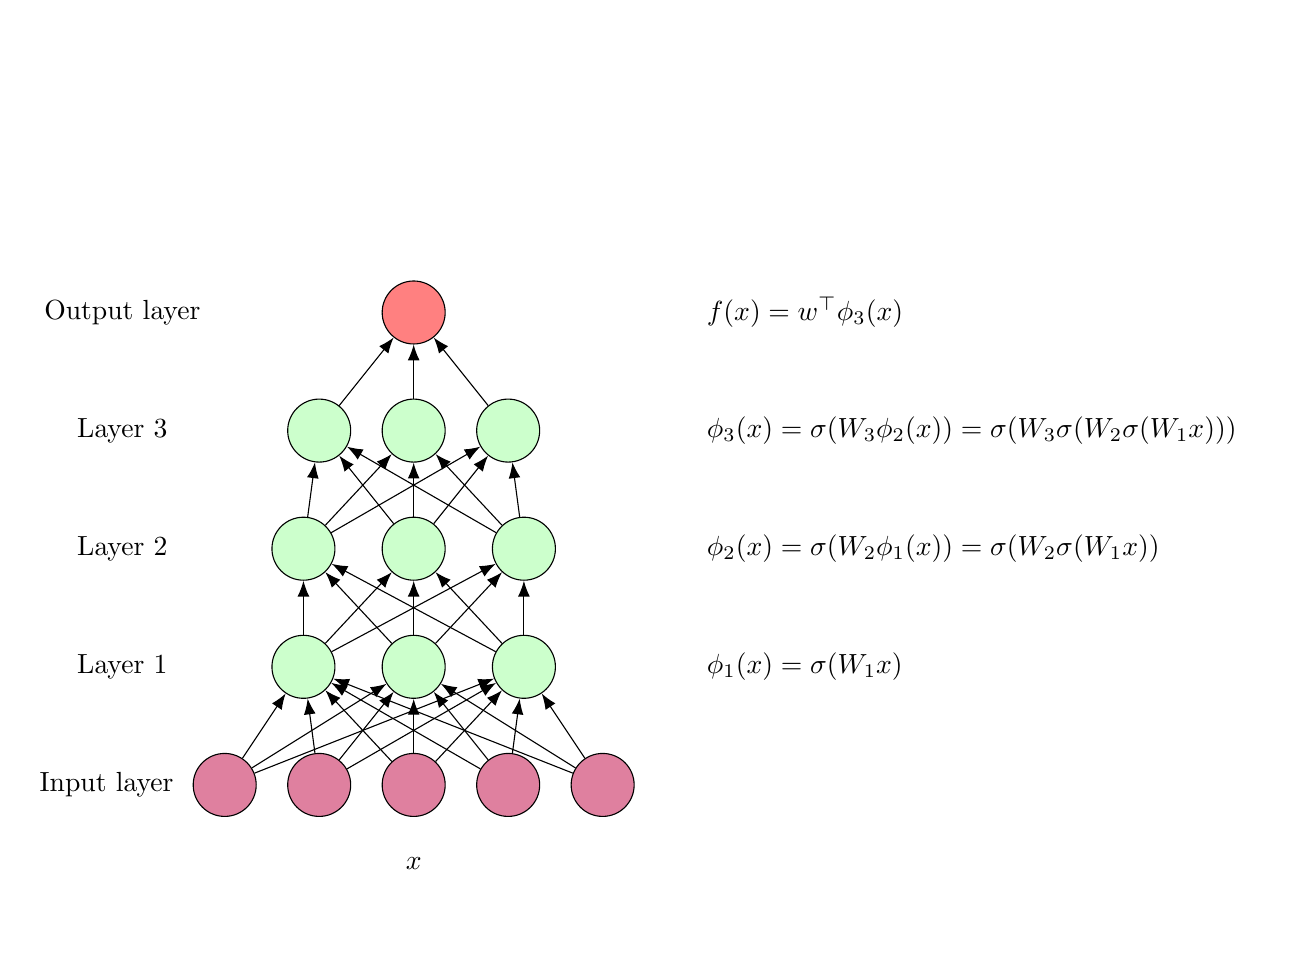
\begin{tikzpicture}[
      node distance=12mm,
      every node/.style={draw,circle,minimum size=8mm},
      input/.style={fill=purple!50},
      hidden/.style={fill=green!20},
      output/.style={fill=red!50},
      arrow/.style={-{Latex[length=2mm]},thin}
  ]

  % INPUT LAYER
  \node[input] (i1) at (0,0)  {};
  \node[input] (i2) at (1.2,0) {};
  \node[input] (i3) at (2.4,0) {};
  \node[input] (i4) at (3.6,0) {};
  \node[input] (i5) at (4.8,0) {};
  \node[draw=none] at (2.4,-1) {$x$};
  \node[draw=none] at (-1.5,0) {Input layer};

  % LAYER 1 (3 nodes)
  \node[hidden] (h11) at (1.0,1.5)  {};
  \node[hidden] (h12) at (2.4,1.5)  {};
  \node[hidden] (h13) at (3.8,1.5)  {};
  \node[draw=none] at (-1.3,1.5) {Layer 1};

  % LAYER 2 (3 nodes)
  \node[hidden] (h21) at (1.0,3.0)  {};
  \node[hidden] (h22) at (2.4,3.0)  {};
  \node[hidden] (h23) at (3.8,3.0)  {};
  \node[draw=none] at (-1.3,3.0) {Layer 2};

  % LAYER 3 (unchanged)
  \node[hidden] (h31) at (1.2,4.5)  {};
  \node[hidden] (h32) at (2.4,4.5)  {};
  \node[hidden] (h33) at (3.6,4.5)  {};
  \node[draw=none] at (-1.3,4.5) {Layer 3};

  % OUTPUT LAYER
  \node[output] (o1) at (2.4,6.0) {};
  \node[draw=none] at (-1.3,6.0) {Output layer};

  % Connections
  \foreach \i in {1,...,5}{
    \foreach \h in {11,12,13}{
      \draw[arrow] (i\i) -- (h\h);
    }
  }
  \foreach \a in {11,12,13}{
    \foreach \b in {21,22,23}{
      \draw[arrow] (h\a) -- (h\b);
    }
  }
  \foreach \a in {21,22,23}{
    \foreach \b in {31,32,33}{
      \draw[arrow] (h\a) -- (h\b);
    }
  }
  \foreach \a in {31,32,33}{
      \draw[arrow] (h\a) -- (o1);
  }

  % Equations on the right
  \node[draw=none,anchor=west,text width=7cm] at (6,4.5)
    {$\phi_3(x)=\sigma(W_3\phi_2(x))=\sigma(W_3\sigma(W_2\sigma(W_1 x)))$};
  \node[draw=none,anchor=west,text width=7cm] at (6,3.0)
    {$\phi_2(x)=\sigma(W_2\phi_1(x))=\sigma(W_2\sigma(W_1 x))$};
  \node[draw=none,anchor=west,text width=7cm] at (6,1.5)
    {$\phi_1(x)=\sigma(W_1 x)$};
  \node[draw=none,anchor=west,text width=7cm] at (6,6.0)
    {$f(x)=w^\top \phi_3(x)$};
  \end{tikzpicture}
}
  \caption{Multi Layer Perceptron with 3 hidden layers}
\end{figure}

Where:
\begin{itemize}
    \item $\boldsymbol{x}$ is the input vector;
    \item $\phi_i(x)$ is the output of layer $i$, learned from the data during training.
    \[\phi_i(x) = \sigma(W_i^T \boldsymbol{x})\]
    \item $W_i$ is the weight matrix of layer $i$. Its dimensions depend on the number of neurons in layer $i$. 
    Each row contains the weights associated to a neuron. Computing $W_i^T \boldsymbol{x}$ will return a vector
    which contains the weighted sum of the inputs for each neuron in layer $i$.
    \item $\sigma(\cdot)$ is a non-linear activation function, applied element-wise.
\end{itemize}
The final output is computed as a linear combination in the new feature space created by the hidden layers.
Differently from SVMs, where the kernel is chosen \textit{a priori}, in MLPs the transformation is learned from data. The only
downside is that training is requires more data and more computational power.
\subsubsection{Activation Functions}
Activation functions introduce non-linearity in the model. We will analyze some proposed functions:

\paragraph{Threshold activation:}
the threshold activation, already seen in the perceptron model, is defined as:
\[ f(\boldsymbol{x}) = sign(\boldsymbol{w}^T \boldsymbol{x}) \]
It's cannot be used in MLPs, since it's derivative is zero almost everywhere, apart from the discontinuity in zero (not differentiable). 
This makes impossible to use gradient-based optimization methods for training.

\paragraph{Sigmoid activation:}
The sigmoid activation function is defined as:
\[ f(\boldsymbol{x}) = \sigma(\boldsymbol{w}^T \boldsymbol{x}) = \frac{1}{1 + e^{-\boldsymbol{w}^T \boldsymbol{x}}} \]
\begin{figure}[H]
    \centering
    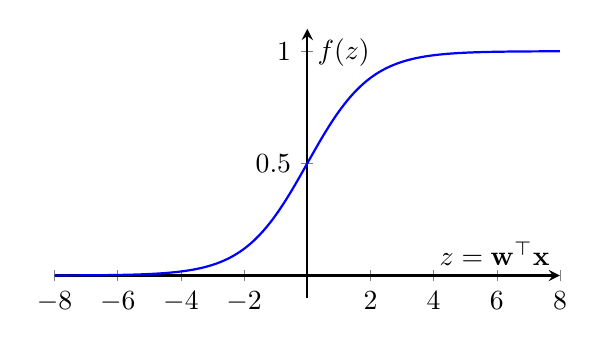
\begin{tikzpicture}
    \begin{axis}[
        axis lines = middle,
        xlabel = {$z = \mathbf{w}^\top \mathbf{x}$},
        ylabel = {$f(z)$},
        ymin = -0.1, ymax = 1.1,
        samples = 200,
        domain = -8:8,
        width=8cm,
        height=5cm,
        thick,
    ]

    \addplot[blue] {1/(1 + exp(-x))};
    \end{axis}
  \end{tikzpicture}
  \caption{Sigmoid activation function}
\end{figure}
It represents a smooth approximation of the threshold function. It is approximately linear around zero, which helps in gradient-based optimization.
However, for large positive or negative values of $z$, the function saturates (approaches 0 or 1), causing the gradient to vanish.

\subsubsection{Output Layer}
The output layer of a neural network produces the final predictions. The function used in this layer can be 
very different from the one used in hidden layers and heavily depends on the task at hand.
\\We will now analyze the activation functions used in the output layer for different tasks.
\paragraph{Binary Classification:} for binary classification tasks, only one output neuron $o(\boldsymbol{x})$ is needed.
The output activation function is usually the sigmoid activation function, which maps the output to the range (0, 1). 
It is defined as:
\[ f(\boldsymbol{x}) = \sigma(o(\boldsymbol{x})) = \frac{1}{1 + e^{-o(\boldsymbol{x})}} \]
This output can be interpreted as the probability of belonging to the positive class.
To obtain the final class label, a threshold (usually 0.5) is applied:
\[ y^* = sign(f(\boldsymbol{x}) - 0.5) \]

\paragraph{Multi-class Classification:} for multi-class classification, similar to what was done with single layer perceptron, a one vs all approach can be used.
This requires $K$ output neurons, one for each class. 
The softmax activation function is commonly used in this case, defined as:
\[ f_i(\boldsymbol{x}) = \frac{\exp(o_i(\boldsymbol{x}))}{\sum_{j=1}^{K} \exp(o_j(\boldsymbol{x}))} \quad \text{for } i = 1, 2, \ldots, K \]
Where $o_i(\boldsymbol{x})$ is the raw output score of the $i$-th output neuron.
\\This function converts the raw output scores into probabilities that sum to 1 across all classes. This is not activated element-wise, but
it is a layer-wise activation function.
The predicted class is the one with the highest probability:
\[ y^* = \arg\max_{i} f_i(\boldsymbol{x}) \] 

\paragraph{Regression:} for regression tasks, where the output is a continuous value, the decision is the value of the output neuron itself.
\[f(\boldsymbol{x}) = o(\boldsymbol{x}) \]

\subsubsection{Representational power of MLPs}
In this section we will analyze the representational power of MLPs on different tasks.
\begin{itemize}
    \item \textbf{Boolean functions:} any boolean function can be represented by a MLP with two layers of units. This can be done using CNF or DNF, but it would require
    an exponential number of hidden units in the worst case;
    \item \textbf{Continuous functions:} any bounded continuous function can be approximated arbitrarily well by a MLP with two layers of units (using sigmoid activations).
    \item \textbf{Arbitrary functions:} any function can be approximated arbitrarily well by a MLP with three layers of units (using sigmoid activations).
\end{itemize}

\subsection{Training Multi Layer Perceptrons}
Similarly to other models, MLPs are trained by minimizing a loss function on the training data. Different loss functions can be used depending on the task at hand.
\subsubsection{Loss Functions}
\paragraph{Binary Classification:}
For binary classification tasks, the binary cross-entropy loss is commonly used. It is defined as:
\[ L(y, f(\boldsymbol{x})) = - (y \log(f(\boldsymbol{x})) + (1 - y) \log(1 - f(\boldsymbol{x}))) \]
This can be interpreted as a switch function between two log-likelihoods, depending on the true label $y$. 
In fact:
\[
  \begin{cases}
  L(y, f(\boldsymbol{x})) = - \log(f(\boldsymbol{x})) & \text{if } y = 1 \\
  L(y, f(\boldsymbol{x})) = - \log(1 - f(\boldsymbol{x})) & \text{if } y = 0
  \end{cases}
\]
This is needed because, as mentioned before, $f(\boldsymbol{x})$ represents the predicted probability of belonging to the positive class. 
\\By putting the minus sign, we convert the maximization problem into a minimization one (from a likelihood to a loss).
This way, making the argument of the log function closest to 1 (correct prediction) will minimize the loss.

\paragraph{Multi-class Classification:}
For multi-class classification tasks, the cross-entropy loss is redefined for multiple classes. It is defined as:
\[ L(y, \boldsymbol{f}(\boldsymbol{x})) = - \log f_y(\boldsymbol{x}) \]
Where $f_y(\boldsymbol{x})$ is the predicted probability for the true class $y$.

\paragraph{Regression:}
For regression tasks, the mean squared error (MSE) loss is commonly used. It is defined as:
\[ L(y, f(\boldsymbol{x})) = (y - f(\boldsymbol{x}))^2 \]

\subsubsection{Stochastic Gradient Descent}
In order to train MLPs, we use Stochastic Gradient Descent (SGD) to minimize the chosen loss function. 
As example, choosing mean squared error (MSE) as loss function, we would have:
\[ E(W) = \frac{1}{2} (y - f(\boldsymbol{x}))^2 \]
Where $W$ represents all the weights in the network. Note that $\frac{1}{2}$ is added to simplify 
the derivative computation.
\\To minimize the loss function, we need to compute the gradient of the loss with respect to each weight in the network.
The relative gradient update is given by:
\[ w_{lj} = w_{lj} - \eta \frac{\partial E(W)}{\partial w_{lj}} \]
Where $\eta$ is the learning rate, $w_{lj}$ is the weight connecting neuron $j$ (source node) 
in the previous layer, to neuron $l$ (target node) in the current layer.
\\To compute the partial derivative can be quite complex when the weights are really far from the output layer, 
where we actually compute the loss (we need the output of the network to compute the loss).
\\To solve this problem, we use the Backpropagation algorithm, which efficiently computes the gradients using the chain rule of differentiation.

\subsubsection{Backpropagation}
The idea behind backpropagation is to compute the gradients layer by layer, starting from the output layer and moving backwards to the input layer.
Since each neuron's output depends on the outputs of the previous layer, which in turn depend on their own weights, we can apply the chain rule to compute the gradients.
\\\\Let's now zoom in on a single node. Suppose we want to compute the gradient of the loss function with respect to a weight $w_{lj}$ 
connecting neuron $j$ in the previous layer to neuron $l$ in the current layer.
\begin{figure}[H]
    \begin{tikzpicture}
        \node[input-node] (x1) at (0, 1.8) {};
        \node (dots) at (0, 1) {$\vdots$};
        \node[input-node, label=above right:$\phi_j$] (pred) at (0, 0) {$x_j$};
        \node (dots) at (0, -0.8) {$\vdots$};
        \node[input-node] (xm) at (0, -1.8) {};
        \node[left=0.5cm of x2] (inputs-label) {Input node $j$};

        % Node l
        \node[circle, draw, minimum size=4cm, label=above:$x_l$] (node_l) at (5, 0) {};
        \node[sum-node] (sum) at (4, 0) {\Large $\Sigma$};
        \node[activation-node, right=1.2cm of sum] (act) {
            \begin{tikzpicture}[scale=0.2] 
                \draw[blue, thick] (-1,-1) -- (0,-1) -- (0,1) -- (1,1); 
            \end{tikzpicture}
        };

        % Connection
        \draw[connection] (x1) -- (sum) node[midway, above] {};
        \draw[connection] (x2) -- (sum) node[midway, above] {$w_{lj}$};
        \draw[connection] (xm) -- (sum) node[midway, above] {};
        \draw[connection] (sum) -- (act) node[midway, above] {$a_l$};
        \draw[connection] (act) -- ++(1,0) node[right] {$\phi_l$};
    \end{tikzpicture}
\end{figure}
The chain rule gives us:
\[
\frac{\partial E(W)}{\partial w_{lj}}
= \underbrace{\frac{\partial E(W)}{\partial a_l}}_{\delta_l}
   \frac{\partial a_l}{\partial w_{lj}}
= \delta_l \, \phi_j
\]
where:
\begin{itemize}
    \item $\delta_l$ represents the error term for neuron $l$. 
    Represents how much the output of neuron $l$ contributes to the final error;
    \item $\phi_j$ is the output of neuron $j$ in the previous layer. It is one of the inputs of the node $l$;
    \item $\frac{\partial a_l}{\partial w_{lj}}$ is the input $\phi_j$. Since $a_l = \sum_{i} w_{li} \phi_i$,
    if we derive with respect to $w_{lj}$ all terms are constant except for the one with $i = j$, which gives $\phi_j$.
\end{itemize}
The final update rule for weight $w_{lj}$ is simply the error term $\delta_l$ multiplied by the input $\phi_j$ coming from the previous layer.
\\The computation of $\delta_l$ depends on whether neuron $l$ is in the output layer or in a hidden layer. We will analyze both cases.

\paragraph{Output layers:}
Since neuron $l$ is in the output layer, we can directly compute the derivative 
of the loss function with respect to the output of the network. Considering the MSE loss function, we have:
\[\delta_{o} = \frac{\partial E(W)}{\partial a_{o}} = \frac{\partial \frac{1}{2} (y - f(\boldsymbol{x}))^2}{\partial a_{o}} \]
Since we do not apply a non-linear activation function in the output layer for regression tasks, we have that $f(\boldsymbol{x}) = a_{o}$, so:
\[ = \frac{\partial \frac{1}{2} (y - a_0)^2}{\partial a_{o}} = -(y - a_{o}) \]

\paragraph{Hidden layers:}
Here the node $l$ is in a hidden layer. Since we compute $\delta_l$ using the chain rule, 
we need to consider the contributions from the neurons in the next layer.
\[\delta_{l} = \frac{\partial E(W)}{\partial a_{l}} = \sum_{k \in \text{children}(l)} \frac{\partial E(W)}{\partial a_{k}} \frac{\partial a_{k}}{\partial a_{l}} \]
Where $k$ are the neurons in the next layer connected to neuron $l$. Intuitively, we are computing the contribution of neuron $l$ to the final error, by considering all the paths from $l$ to the output layer.
\\The term $\frac{\partial E(W)}{\partial a_{k}}$ is simply $\delta_k$, already computed in the next layer. We derive that:
\[\delta_{l} = \sum_{k \in \text{children}(l)} \delta_k \frac{\partial a_{k}}{\partial a_{l}} \]
Remembering that $a_k = \sum_{m} w_{km} \phi_m$, where $\phi_m$ is the output of neuron $m$ in the previous layer, we have that:
\[\frac{\partial a_{k}}{\partial a_{l}} = \frac{\partial a_{k}}{\partial \phi_{l}} \frac{\partial \phi_{l}}{\partial a_{l}}\]
The first term is simply the weight $w_{kl}$. The second term is the derivative of the activation function $\sigma(\cdot)$ used in neuron $l$.
Putting everything together, we have:
\[\delta_{l} = \sum_{k \in \text{children}(l)} \delta_k w_{kl} \sigma(a_{l})(1 - \sigma(a_{l})) \]
Where we used the derivative of the sigmoid activation function $(\frac{\partial \sigma(x)}{\partial x} = \sigma(x)(1 - \sigma(x)))$.

\subsection{Modular Structure of Neural Networks}
Neural networks can be seen as a combination of different modules, each with a specific function. Each of these modules has an interface to communicate with other modules.
Each layer $j$ takes as input  $\phi_{j-1}$ and it's weights $W_j$, and produces as output $\phi_{j} = F(\phi_{j-1}, W_j)$. Once we get to the output layer, we can compute the loss function and the gradients using backpropagation.
\[\frac{\partial E(W)}{\partial W_j} = \frac{\partial E(W)}{\partial \phi_j} \frac{\partial \phi_j}{\partial W_j}  = \frac{\partial E(W)}{\partial \phi_j} \frac{\partial F_j(\phi_{j-1}, W_j)}{\partial W_j}\]
Each layer computes:
\[ \frac{\partial E(W)}{\partial \phi_{j-1}} = \frac{\partial E(W)}{\partial \phi_j} \frac{\partial \phi_j}{\partial \phi_{j-1}} = \frac{\partial E(W)}{\partial \phi_j} \frac{\partial F_j(\phi_{j-1}, W_j)}{\partial \phi_{j-1}} \]
Each module must be able to compute:
\begin{itemize}
    \item the derivative of its output with respect to its weights:
    \[ \frac{\partial \phi_j}{\partial W_j} = \frac{\partial F_j(\phi_{j-1}, W_j)}{\partial W_j} \]
    \item the derivative of its output with respect to its input:
    \[ \frac{\partial \phi_j}{\partial \phi_{j-1}} = \frac{\partial F_j(\phi_{j-1}, W_j)}{\partial \phi_{j-1}} \]
\end{itemize}

\subsection{Remarks on Training Neural Networks}
The error surface of neural networks is non-convex. This implies that there can be multiple local minima and backpropagation is only guaranteed to find a local minimum.
There are many techniques to improve the training of neural networks, that we will cover later in this section.
\subsubsection{Stopping Criteria}
Overtraining the network can increase the possibility of overfitting the training data. When the network is initialized, the weights are set to small random values. In this phase, we have a very simple surface, which is easy to optimize.
\\As the weights are updated, the surface becomes more complex, and the risk of overfitting increases.
To avoid this, a separate validation set is used to monitor the performance of the network during training. When the performance on the validation set starts to degrade, training is stopped.
\subsubsection{Vanishing gradients}
A common problem when training deep neural networks is the vanishing gradient problem. During backpropagation, at each step the 
gradient is multiplied by the derivative of the activation function (sigmoid in our case). 
Since the saturated regions of the sigmoid have very small derivatives, the gradients can become very small as they are propagated back through the layers.
A few simple suggestions to mitigate this problem are:
\begin{itemize}
    \item \textbf{Weight initialization:} initialize the weights to small random values;
    \item \textbf{Normalization:} normalize the input data to have zero mean and unit variance ($X' = \frac{X - \mu_x}{\sigma_x}$)
\end{itemize}
Other tricks of the trade will be covered in the next paragraph.
\paragraph{Activations functions:}
Since the main problem generating vanishing gradients is the use of the sigmoid activation function, a new activation function has been proposed: the ReLU (Rectified Linear Unit).
It is defined as:
\[ f(x) = \max(0, \boldsymbol{w}^T \boldsymbol{x}) \]
Where $\boldsymbol{w}^T \boldsymbol{x}$ represents the weighted sum of inputs to the neuron.
\begin{center}
\begin{tikzpicture}
\begin{axis}[
    axis lines = middle,
    xlabel = {$z = \mathbf{w}^\top \mathbf{x}$},
    ylabel = {$f(z)$},
    ymin = -1, ymax = 6,
    samples = 200,
    domain = -4:4,
    width=10cm,
    height=6cm,
    thick,
]
\addplot[blue] {(x > 0) * x};
\end{axis}
\end{tikzpicture}
\end{center}
The ReLU activation function does not saturate for positive values, and its derivative is constant (1) in that region. This helps to mitigate the vanishing gradient problem.

\paragraph{Regularization:}
Two common regularization techniques used in training neural networks are:
\begin{itemize}
  \item \textbf{2-norm regularization:} adding a penalty term to the loss function proportional to the euclidean norm of the weights.
  \[ J(W) = E(W) + \lambda ||W||_2 \]
  In essence, this encourages less relevant weights to be small, reducing overfitting.
  \item \textbf{1-norm regularization:} adding a penalty term to the loss function proportional to the absolute value of the weights.
  This encourages less relevant weights to be exactly zero.
  \[ J(W) = E(W) + \lambda |W| \]
\end{itemize}

\paragraph{Initialization:}
Random initialization of weights is crucial for braking symmetry between neurons. If all weights are initialized to the same value, all neurons in a layer will learn the same features.
A common approach is to initialize weights randomly, from a uniform distribution in the range:
\[ W_{ij} \sim U\left(-\frac{\sqrt{6}}{\sqrt{n + m}}, \frac{\sqrt{6}}{\sqrt{n + m}}\right) \]
Where $n$ is the number of input units and $m$ is the number of output units.

\paragraph{Gradient descent:}
\begin{itemize}
  \item \textbf{Batch Gradient Descent:} updates weights after seeing the entire training set. This can be computationally expensive for large datasets;
  \item \textbf{Stochastic Gradient Descent:} updates weights after seeing each training example. The final objective function is noisy and may be different from the true objective;
  \item \textbf{Mini-batch Gradient Descent:} updates weights after seeing a small batch of training examples. The size of the batch is usually associated with the hardware capabilities (e.g., GPU memory). 
\end{itemize}

\paragraph{Momentum:}
Momentum is a technique used to accelerate gradient descent and escape local minima. The idea is to update the weights using
a combination of the current gradient and the previous updates, similar to a ball rolling down a hill.
The update rule with momentum is given by:
\[v_{ji}^\text{(new)} = \alpha v_{ji}^\text{(old)} - \eta \frac{\partial E(W)}{\partial w_{ji}}\]
\[w_{ji}^\text{(new)} = w_{ji}^\text{(old)} + v_{ji}^\text{(new)}\]
Where:
\begin{itemize}
    \item $\alpha$ is the momentum coefficient. $0 \le \alpha < 1$
    \item $v_{ji}$ is the velocity term for weight $w_{ji}$;
\end{itemize}

\paragraph{Adaptive Learning Rates:}
Adaptive learning rate methods adjust the learning rate during training based on the progress made.
Some popular methods are:
\begin{itemize}
    \item \textbf{Decreasing learning rate:} gradually decrease the learning rate over time.
    \[\eta_t = \begin{cases}
    (1 - \frac{t}{\tau})\eta_0 + \frac{t}{\tau} \eta_{\text{min}}  & \text{if } t < \tau \\
    \eta_{\text{min}} & \text{if } t \ge \tau
    \end{cases}
    \]
    The idea is to start with a high learning rate to explore the error surface, and then decrease to avoid oscillations around minima.
    The learning rate is decreased linearly from $\eta_0$ to $\eta_{\text{min}}$ over $\tau$ iterations. After that, it remains constant at $\eta_{\text{min}}$;
    \item \textbf{AdaGrad:} adapts the learning rate for each weight based on the historical gradients.
    \[ r_{ji}^\text{(new)} = r_{ji}^\text{(old)} + \left(\frac{\partial E(W)}{\partial w_{ji}}\right)^2 \]
    \[ w_{ji}^\text{(new)} = w_{ji}^\text{(old)} - \frac{\eta}{\sqrt{r_{ji}^\text{(new)}}} \frac{\partial E(W)}{\partial w_{ji}} \]
    Where $r_{ji}$ accumulates the squared gradients for weight $w_{ji}$. This results in smaller updates for weights with large gradients (steep directions) and larger updates for weights with small gradients (flat directions);
    This has a drawback: the accumulated squared gradients can grow indefinitely.
    \item \textbf{RMSProp:} addresses the drawback of AdaGrad by using an exponentially decaying average of squared gradients.
    \[ r_{ji}^\text{(new)} = \rho r_{ji}^\text{(old)} + (1 - \rho) \left(\frac{\partial E(W)}{\partial w_{ji}}\right)^2 \]
    \[ w_{ji}^\text{(new)} = w_{ji}^\text{(old)} - \frac{\eta}{\sqrt{r_{ji}^\text{(new)} + \epsilon}} \frac{\partial E(W)}{\partial w_{ji}} \]
    Where $\rho$ allows to exponentially decay the influence of past gradients.
\end{itemize}
\paragraph{Batch Normalization:}
To mitigate the problem of internal covariate shift, batch normalization is used. It normalizes the input of each activation function on its mini-batch.
\[ \hat{x_i} = \frac{x_i - \mu_B}{\sigma_B}\]
Where $\mu_B$ and $\sigma_B$ are the mean and standard deviation of the mini-batch $B$, $x$ is the activation of an arbitrary layer.
This normalization helps to stabilize the learning process and allows for higher learning rates.
\subsection{Popular architectures}
Different architectures of neural networks have been proposed to tackle specific problems. In this section we will briefly describe some of the most popular ones.
\subsubsection*{Autoencoders}
Autoencoders are a type of neural network used for unsupervised learning (learning with no labelled data). They consist of an
encoder, that maps the input data to a lower-dimensional latent space, and a decoder, that reconstructs the input data from the latent representation.
This is useful for dimensionality reduction, feature learning, and data compression.
\subsubsection*{Convolutional Neural Networks (CNNs)}
Convolutional Neural Networks (CNNs) are specialized neural networks designed for processing grid-like data, such as images. 
They use convolutional filters to extract local features from the input data. Pooling layers are used to compose higher-level features from lower-level ones.
After several convolutional and pooling layers, fully connected layers are used to perform the final classification.
\subsubsection*{Generative Adversarial Networks (GANs)}
Generative Adversarial Networks (GANs) learns to generate items from random noise. 
They consist of two neural networks: a generator, that generates new data, and a discriminator, that tries to distinguish between real and generated data.
The two networks are trained simultaneously, with no supervision needed.
\subsubsection*{Transformers}
Use attention mechanisms to learn input words encodings, that depends on the context of the sentence.
They can also learn output words encodings, that depends on the context of the already generated words and on the input sentence.
\subsubsection*{Graph Neural Networks (GNNs)}
Allow to learn from graph-structured data. Allow to propagate information from a node to its neighbors, learning a representation that takes into account the graph structure.

\section{Unsupervised Learning - Clustering}
What we have seen so far are all examples of \textbf{supervised learning}, which required a labeled dataset to learn from. This process
is usually extremely expensive and it could happen that we don't have access to labeled data at all. 
\\In such cases, we can resort to \textbf{unsupervised learning} techniques, which can be used to group data points into \textbf{clusters}. 

\subsection{K-Means Clustering}
One of the most popular clustering algorithms is \textbf{K-Means Clustering}. The setting is the following:
\begin{itemize}
    \item We have a dataset of $n$ points $\{x_1, x_2, \ldots, x_n\}$ in $\mathbb{R}^d$.
    \item We assume that examples should be grouped into $k$ clusters, we will see later how to choose $k$;
    \item Each cluster $i$ is represented by its \textbf{centroid} (mean) $\mu_i$;
\end{itemize}
\subsubsection*{Algorithm}
The K-Means algorithm works as follows:
\begin{enumerate}
    \item Initialize $k$ cluster means $\mu_1, \mu_2, \ldots, \mu_k$ (randomly or using some heuristic);
    \item Repeat until convergence:
    \begin{itemize}
        \item \textbf{Assignment step}: Assign each point $x_j$ to the nearest cluster mean;
        \item \textbf{Update step}: Update cluster means according to the assigned points;
    \end{itemize}
\end{enumerate}
The algorithm converges when the assignments no longer change or the cluster means stabilize. 
\subsubsection*{Distance Metrics}
To compute the distance between points and cluster means, we have to choose a distance metric, the most common choices are:
\begin{itemize}
    \item Euclidean distance in $\mathbb{R}^d$;
    \[d(\boldsymbol{x}, \boldsymbol{x}') = \sqrt{\sum_{i=1}^d (x_i - x_i')^2}\]
    \item Manhattan distance:
    \[d(\boldsymbol{x}, \boldsymbol{x}') = \sum_{i=1}^d |x_i - x_i'|\]
    \item Cosine similarity:
    \[d(\boldsymbol{x}, \boldsymbol{x}') = 1 - \frac{\boldsymbol{x}^T  \boldsymbol{x}'}{||\boldsymbol{x}|| \, ||\boldsymbol{x}'||}\]
\end{itemize}
\subsection{Quality of Clustering}
Since we are working in an unsupervised setting, we don't have labels to evaluate the quality of our clustering. However, we can define the following metrics:
\defib{Sum-of-Squared error criterion}
{
    The sum-of-squared error criterion is defined as:
    \begin{itemize}
        \item let $n_i$ be the number of points assigned to cluster $i$ ($D_i$);
        \item let $\mu_i$ be the centroid of cluster $i$. It can be computed as:
        \[\mu_i = \frac{1}{n_i} \sum_{\boldsymbol{x} \in D_i} \boldsymbol{x}\]
        \item the sum-of-squared error criterion is defined as:
        \[ E = \sum_{i=1}^k \sum_{\boldsymbol{x} \in D_i} ||\boldsymbol{x} - \mu_i||^2 \]
    \end{itemize}
    It measures the squared error incurred in representing each point by its cluster centroid.
}
\subsection{Gaussian Mixture Models (GMM)}
The idea behind Gaussian Mixture Models is to model the data as a mixture of several Gaussian distributions. 
Each cluster is represented by a Gaussian distribution with its own parameters (mean and covariance).
It assumes that the number of clusters $K$ is given and that each data point is generated from one of the $K$ Gaussian distributions.
\subsubsection*{Parameter Estimation}
If we wanted to estimate the parameters of the Gaussians (means and covariances), we could use Maximum Log-Likelihood Estimation (MLE).
\[ \theta^* = \arg \max_{\theta} \mathcal{L}(\theta|\mathcal{D})\]
where $\theta$ are the parameters of the Gaussians and $\mathcal{D}$ is the dataset.
\[ \mathcal{L}(\theta|\mathcal{D}) = \sum_{i=1}^{n} \log \left( \sum_{h = 1}^{K}p(x_i | \theta_k) \right) \]
However, MLE cannot be used directly, since the cluster assignments are unknown.
Instead, we can apply an iterative approach called the \textbf{Expectation-Maximization (EM)}.

\subsubsection*{Expectation-Maximization (EM) Algorithm}
The EM algorithm consists of two main steps:
\begin{enumerate}
    \item \textbf{E-step (Expectation step)}: Compute the expected cluster assignments given the current parameters;
    \item \textbf{M-step (Maximization step)}: Update the parameters of the Gaussians given the expected cluster assignments;
    \item Repeat until convergence.
\end{enumerate}
\subsubsection*{Example: estimating the mean of k univariate Gaussians}
Here, we assume to have a dataset of $x_1, x_2, \ldots, x_n$ examples.
We assume that the data is generated from $k$ univariate Gaussian distributions with 
unknown means $\mu_1, \mu_2, \ldots, \mu_k$ and known variance $\sigma^2$.
We want to estimate the means of the Gaussians using, allowing us to assign points to clusters probabilistically.
\\The algorithm works as follows:
\begin{enumerate}
    \item \textbf{Initialization}: randomly initialize the means $h = \langle\mu_1, \mu_2, \ldots, \mu_k \rangle$;
    \item \textbf{Iterate until convergence}: convergence is checked by measuring the change in Maximum Log-Likelihood:
    \begin{itemize}
        \item \textbf{E-step}: compute the posterior probability that a datapoint $x_i$ belongs to cluster $j$, 
        given the current means $h$.
        \[ \gamma_{ik} = \frac{\pi_k p(x_i | \mu_k)}{\sum_{j=1}^{k} \pi_j p(x_i | \mu_j)} \]
        We are basically computing the probability that $x_i$ belongs to cluster $j$ and normalizing it over all clusters for each data point.
        This way, summing over all clusters gives $1$.
        The term $\pi_j$ represents the prior probability of cluster $j$.
        \\Since we are working with Gaussians, we use the Gaussian probability density function to compute $p(x_i | \mu_j)$.
        \[ = \frac{\pi_k\exp - \frac{1}{2\sigma^2}(x_i - \mu_k)^2}{\sum_{j=1}^{K}\exp - \frac{1}{2\sigma^2}(x_i - \mu_j)^2} \]
        \item \textbf{M-step}: calculate a new hypotesis $h'$ assuming values of latent variables are their expected values.
        The maximum likelihood estimate of the mean $\mu_j$ is given by the weighted sample mean, where each istance is weighted by its probability of
        belonging to cluster $j$:
        \[ \mu_j' = \frac{\sum_{i=1}^{n} \gamma_{ik} x_i}{\sum_{i=1}^{n} \gamma_{ik}} \]
    \end{itemize}
\end{enumerate}

\subsection{Choose the number of clusters k}
Choosing the right number of clusters $k$ is a crucial step in clustering. Increasing the number of clusters will always
improve the fit to the data, but it may lead to overfitting. We will now introduce different methods to choose $k$.

\subsubsection{Elbow Method}
The Elbow Method tries to trade-off the quality of the clustering with quantity. The number of clusters $k$ should stop 
increasing when the advantage of adding another cluster is limited.
The approach is composed of the following steps:
\begin{itemize}
    \item Run the clustering algorithm for increasing values of $k$;
    \item For each $k$, compute the sum-of-squared error criterion $E(k)$;
    \item Plot $E(k)$ against $k$;
    \item Choose $k$ at the "elbow" point, where the decrease in $E(k)$ starts to slow down.
\end{itemize}
\begin{figure}[H]
    \centering
    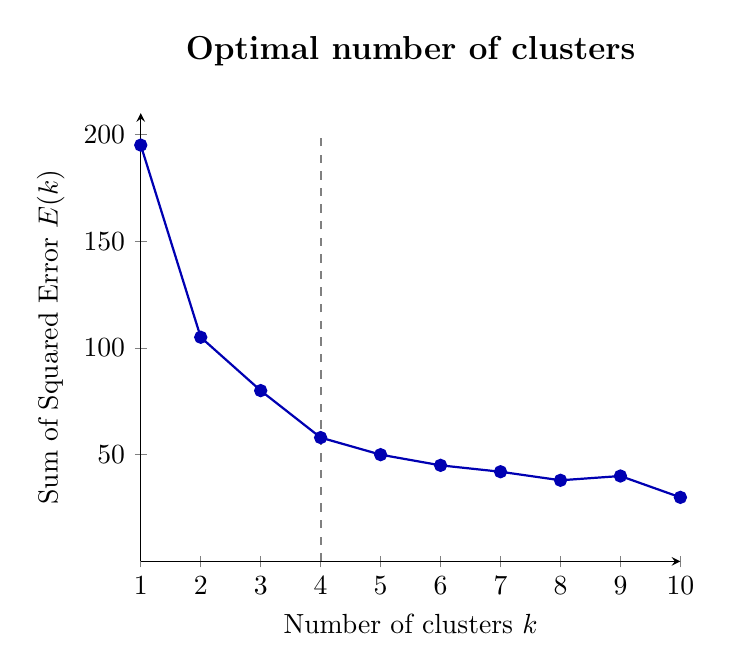
\begin{tikzpicture}
    \begin{axis}[
        title={Optimal number of clusters},
        xlabel={Number of clusters $k$},
        ylabel={Sum of Squared Error $E(k)$},
        xmin=1, xmax=10,
        ymin=0, ymax=210,
        xtick={1,2,3,4,5,6,7,8,9,10},
        ytick={50,100,150,200},
        grid=none,
        axis lines=left,
        title style={at={(0.5,1.1)}, anchor=center, font=\bfseries\large},
    ]
    % The Data Points
    \addplot[color=blue!70!black,mark=*,thick,]
    coordinates {
        (1,195) (2,105) (3,80) (4,58) (5,50) (6,45) (7,42) (8,38) (9,40) (10,30)
    };
    % The Vertical Dashed "Elbow" Line at k=4
    \draw [dashed, thick, gray] (axis cs:4,0) -- (axis cs:4,200);
    \end{axis}
    \end{tikzpicture}
    \caption{Elbow Method example plot. The elbow point is at $k=4$.}
\end{figure}
This method is really intuitive, but can be ambiguous, since the elbow point is not always clear.
For example, in the plot above, one could argue that $k=2$ or $k=3$ are also valid choices.

\subsubsection{Silhouette Method}
Increasing the number of clusters $k$ will always decrease the sum-of-squared error criterion, but it will also increase the 
similarity between different clusters. The Silhouette Method tries to balance these two aspects.
The silhouette score for a single point $x_i$ is defined as:
\begin{itemize}
    \item $a(i)$: average distance between $x_i$ and all other points in the same cluster $C$:
    \[ a(i) = \frac{1}{|C|} \sum_{j \in C} d(i, j) \]
    \item $b(i)$: minimum average distance between $x_i$ and all points in any other cluster $C'$:
    \[ b(i) = \min_{C' \neq C} \frac{1}{|C'|} d(i, C') \]
    \item The silhouette score $s(i)$ is then defined as:
    \[ s(i) = \frac{b(i) - a(i)}{\max(a(i), b(i))} \]
\end{itemize}
To choose the number of clusters $k$, we compute the average silhouette score over all points for different values of $k$. As before,
we plot the average silhouette score against $k$ and choose the value of $k$ that maximizes the score.
\begin{figure}[H]
    \centering
    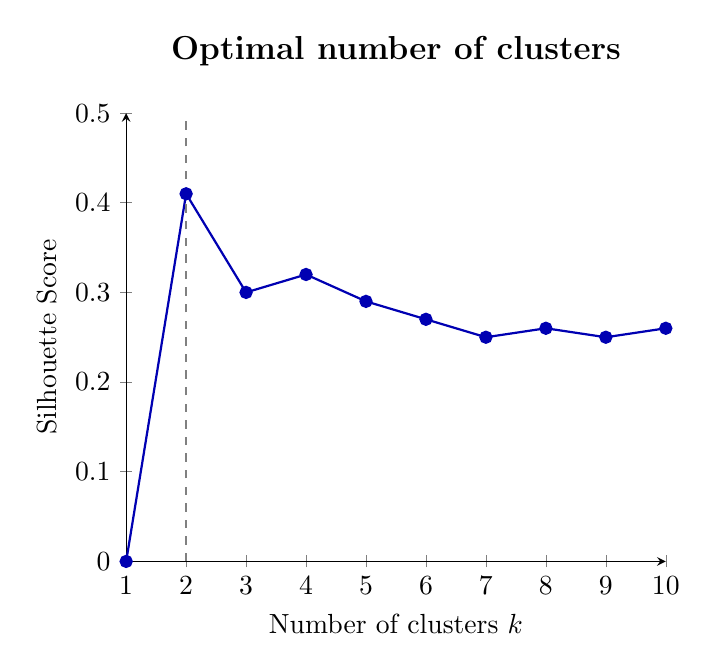
\begin{tikzpicture}
    \begin{axis}[
        title={Optimal number of clusters},
        xlabel={Number of clusters $k$},
        ylabel={Silhouette Score},
        xmin=1, xmax=10,
        ymin=0, ymax=0.5,
        xtick={1,2,3,4,5,6,7,8,9,10},
        ytick={0,0.1,0.2,0.3,0.4,0.5},
        grid=none,
        axis lines=left,
        title style={at={(0.5,1.1)}, anchor=center, font=\bfseries\large},
    ]
    % The Data Points
    \addplot[color=blue!70!black,mark=*,thick,]
    coordinates {
        (1,0.0) (2,0.41) (3,0.3) (4,0.32) (5,0.29) (6,0.27) (7,0.25) (8,0.26) (9,0.25) (10,0.26)
    };
    % The Vertical Dashed "Elbow" Line at k=4
    \draw [dashed, thick, gray] (axis cs:2,0) -- (axis cs:2,0.5);
    \end{axis}
    \end{tikzpicture}
    \caption{Silhouette Method example plot. The optimal number of clusters is at $k=2$.}
\end{figure}
\subsubsection{Hierarchical Clustering}
Hierarchical Clustering is an alternative approach, that assumes that the data is organized in a hierarchy of clusters.
This structure can be built from examples in two ways:
\begin{itemize}
    \item \textbf{Top-down approach}: start with all data points in a single cluster and recursively split clusters into smaller clusters;
    \item \textbf{Bottom-up approach}: start with each data point in its own cluster and recursively merge clusters into larger clusters.
\end{itemize}
The algorithm for the Bottom-up approach is defined as follows:
\begin{itemize}
    \item Initialize:
    \begin{itemize}
        \item Set the target number of clusters $k$;
        \item Set the initial number $\hat{k}$ of clusters to $n$;
        \item Initialize clusters as individual data points: $D_i = \{x_i\}, \forall i \in [1, n]$
    \end{itemize}
    \item Repeat until the number of clusters $\hat{k}$ is equal to $k$:
    \begin{itemize}
        \item Find the two closest clusters $D_i$ and $D_j$;
        \item Merge the clusters: $D_i \leftarrow D_i \cup D_j$;
        \item Update the number of clusters: $\hat{k} \leftarrow \hat{k} - 1$;
    \end{itemize}
\end{itemize}
The similarity between clusters can be computed in different ways:
\begin{itemize}
    \item \textbf{Nearest neighbor}: distance between the two closest points in the clusters:
    \[ d_{min}(D_i, D_j) = \min_{\boldsymbol{x} \in D_i, \boldsymbol{x'} \in D_j} ||\boldsymbol{x} - \boldsymbol{x'}|| \]
    \item \textbf{Farthest neighbor}: distance between the two farthest points in the clusters:
    \[ d_{max}(D_i, D_j) = \max_{\boldsymbol{x} \in D_i, \boldsymbol{x'} \in D_j} ||\bold{x} - \boldsymbol{x'}|| \]
    \item \textbf{Average linkage}: average distance between all points in the clusters:
    \[ d_{avg}(D_i, D_j) = \frac{1}{|D_i| |D_j|} \sum_{\boldsymbol{x} \in D_i} \sum_{\boldsymbol{x'} \in D_j} ||\boldsymbol{x} - \boldsymbol{x'}|| \]
\end{itemize}
The first two methods are sensitive to outliers, while the average linkage is more robust. All result complex to compute. A more efficient method is the \textbf{centroid method}, which computes the distance between the centroids of the clusters:
\[ d_{centroid}(D_i, D_j) = ||\mu_i - \mu_j|| \]
where $\mu_i$ and $\mu_j$ are the centroids of clusters $D_i$ and $D_j$ respectively.

\section{Reinforcement Learning}
Reinforcement Learning (RL) is a type of machine learning where an agent learns to make decisions by taking actions in an environment to maximize cumulative rewards.
\subsection{Learning Settings}
\begin{itemize}
    \item The learner (agent) is provided with a set of possible states $S$, and for each state, a set of possible actions $A$, moving it to a new state.
    \item In performing action $a$, from state $s$, the agent receives an immediate reward $r$.
    \item The goal is to learn a policy $\pi: S \rightarrow A$ that maximizes the overall reward over time.
    \item The learner has to deal with problems of dealayed reward, where the consequences of an action may not be immediately apparent and trade-offs between exploration (trying new actions) and exploitation (choosing actions known to yield high rewards).
\end{itemize}
More formally, the setting of reinforcement learning can be modeled as a Markov Decision Process (MDP).
\subsection{Markov Decision Process (MDP)}
An MDP is defined by:
\begin{itemize}
    \item A set of \textbf{states} $S$, in which the agent can be;
    \item A set of \textbf{terminal states} $S_{G} \subseteq S$, where the process ends. Might also be empty;
    \item A set of \textbf{actions} $A$ available to the agent;
    \item A \textbf{transition model}, providing the probability of going to state $s'$ when taking action $a$ in state $s$: 
    \[
        P(s'|s,a) ; s,s' \in S, a \in A
    \]
    \item A \textbf{reward function} $R(s,a,s')$, providing the immediate reward received after transitioning from state $s$ to state $s'$ due to action $a$.
\end{itemize}
The agent's objective is to find a policy $\pi(s)$ that maximizes an utility function, taking into account the uncertainty in state transitions and rewards.

\subsection{Utilities}
Utilities are defined over environment histories. An environment history is a sequence of states $[s_0, s_1, s_2, ...]$, passed through by the agent.
When calculating the utility, we assume an infinite horizon, meaning the agent will continue to interact with the environment indefinitely. We also assume stationary preferences, meaning the agent's preferences do not change over time.
\\We can define the utility in two ways:
\begin{itemize}
    \item \textbf{Additive rewards}: values immediate and future rewards equally.
    \[ U([s_0, s_1, s_2, \dots]) = R(s_0) + R(s_1) + R(s_2) + \dots \]
    \item \textbf{Discounted utility}: prefers immediate rewards over future rewards.
    \[ U([s_0, s_1, s_2, \dots]) = R(s_0) + \gamma R(s_1) + \gamma^2 R(s_2) + \dots \]
    where $0 \leq \gamma < 1$ is the discount factor.

\end{itemize}
Here we are assuming that rewards only depend on the current state, not the action taken or the next state.

\subsection{Policy}
A policy $\pi$ is a mapping from states to actions: $\pi: S \rightarrow A$. It defines the action that the agent should take when in a given state.
\paragraph{Expected Utility of a policy}
Given a policy $\pi$, we define the expected utility of $\pi$ as the utility of an environment, taken in expectation over all possible state sequences generated by following policy $\pi$.
In other words, we are multiplying the utility of that history, by the probability of that history occurring under policy $\pi$.
\defib{Optimal Policy}{
An optimal policy $\pi^*$ is a policy that maximizes the expected utility. In other words, it is the best policy the agent can follow to achieve the highest cumulative reward over time.
}
\defib{Utility of states}{
    Given a policy $\pi$, the utility of a state $s$ is defined as:
    \[
        U^{\pi}(s) = \mathbb{E}_{\pi} \left[ \sum_{t = 0}^{\inf} \gamma^t R(S_t)|S_0 = s \right]
    \]
    Where $S_t$ is the state reached after $t$ steps, using policy $\pi$, starting from state $S_0 = s$.
    This is the expected utility of the environment history, starting from state $s$ and following policy $\pi$.
}
We can define the \textbf{true utility} of a state $s$, under the optimal policy $\pi^*$, as:
\[ U^*(s) = U^{\pi^*}(s) \]
Given the true utility of each state, we can easily derive the optimal policy by choosing the action that maximizes the expected utility:
\label{optpolicy}
\[\pi^*(s) = \arg\max_{a \in A} \sum_{s' \in S} P(s'|s,a) U(s') \]
This definition creates a circular dependency between the optimal policy and the true utility, which can be resolved using the Bellman equations.

\subsubsection{Bellman Equations}
The Bellman equation for state $s$ is defined as:
\[ U(s) = R(s) + \gamma \max_{a \in A} \sum_{s' \in S} P(s'|s,a) U(s') \]
This equation states that the utility of a state $s$ is equal to the immediate reward $R(s)$ plus the discounted expected utility of the next state, assuming the agent takes the optimal action.
We can define a system of Bellman equations, one for each state in the MDP. Solving this system will yield the true utilities for all states, which can then be used to derive the optimal policy.
Directly solving this system can be computationally expensive, since they are non-linear equations. Instead, we can use iterative methods such as value iteration or policy iteration to approximate the solution.

\subsubsection{Value Iteration }
Value iteration, also known as Utility Iteration, works by initializing the utility of all states to arbitrary values (for example zero) and then repeatedly updating the utilities using the Bellman equation until convergence.
\begin{algorithm}[H]
    \caption{Value Iteration}
    \begin{algorithmic}[1]
        \State Initialize $U_0(s) \forall s \in S$ to 0
        \Repeat
            \State Update $U_{i+1}(s)$ using the Bellman equation:
            \[
            U_{i+1}(s) \leftarrow R(s) + \gamma \max_{a \in A} \sum_{s' \in S} P(s'|s,a) U_i(s')
            \]
            \State $i \leftarrow i + 1$
        \Until{convergence}
        \State \textbf{return} $U(s)$
    \end{algorithmic}
\end{algorithm}
At each iteration, we update the utility of each state based on the current estimates of the utilities of the successor states. This process continues until the utilities converge to stable values.
The policy can then be derived from the converged utilities using the formula for the optimal policy \ref{optpolicy}.

\subsubsection{Policy Iteration}
Contrary to what happens in value iteration, in policy iteration we start with an arbitrary policy and then iteratively improve it.
\begin{algorithm}[H]
    \caption{Policy Iteration}
    \begin{algorithmic}[1]
        \State Initialize an arbitrary policy $\pi_0$ randomly
        \Repeat
            \State \textbf{Policy Evaluation}: solve the set of linear equations:
            \[
                U_i(s) = R(s) + \gamma \sum_{s' \in S} P(s'|s, \pi_i(s)) U_i(s') \;\; \forall s \in S
            \]
            where $\pi_i(s)$ is the action taken in state $s$ under policy $\pi_i$.
            \State \textbf{Policy Improvement}: update the policy using the new utilities:
            \[
                \pi_{i+1}(s) = \arg\max_{a \in A} \sum_{s' \in S} P(s'|s,a) U_i(s') \;\; \forall s \in S
            \]
        \Until{convergence}
        \State \textbf{return} $\pi(s)$
    \end{algorithmic}
\end{algorithm}
In the policy evaluation step, we compute the utilities of the states under the current policy by solving a system of linear equations. Using the current policy, instead of the max operator from the Bellman equation,
we made the equations linear, making it easier to solve.
In the policy improvement step, we update the policy using equation \ref{optpolicy}, based on the newly computed utilities.

\subsection{Dealing with Partial Knowledge}
Value iteration and policy iteration both assume that the agent has complete knowledge of the MDP.
In most real-world scenarios, the agent does not have access to the full transition model or reward function, but it aims to learn them through interaction with the environment.
\\There are two main approaches to deal with this partial knowledge:
\begin{itemize}
    \item \textbf{Policy Evaluation}: the policy is given, environment is learned through experience;
    \item \textbf{Policy Improvement}: both the policy and the environment are learned through experience.
\end{itemize}
\subsubsection{Adaptive Dynamic Programming (ADP)}
In ADP, the agent maintains counts of visited state and states, given action taken and previous state. These counts are used to do maximum likelihood estimation of the transition model.
\begin{algorithm}
    \caption{Adaptive Dynamic Programming}
    \begin{algorithmic}
        \Repeat
            \State Initialize $s$
            \Repeat
                \State receive reward $r$, set R($s$) = r
                \State choose action $a \leftarrow \pi(s)$
                \State execute action $a$, observe next state $s'$
                \State update counts:
                \[
                    N(s,a) \leftarrow N(s,a) + 1
                \]
                Where $N(s,a)$ is the number of times action $a$ has been taken in state $s$.
                \[
                    N(s'| s,a) \leftarrow N(s'| s,a) + 1
                \]
                Where $N(s'| s,a)$ is the number of times action $a$ has led to state $s'$ from state $s$.
                \State update transition model:
                \[
                    P(s''|s,a) = \frac{N(s''| s,a)}{N(s,a)} \;\; \forall s'', s \in S, a \in A
                \]
                This is the maximum likelihood estimate of the transition probabilities.
                \State update utilities using policy evaluation
                \State $U \leftarrow \text{PolicyEvaluation}(\pi,U, p, R, \gamma)$
            \Until{$s$ is terminal}
        \Until{convergence}
    \end{algorithmic}
\end{algorithm}
The algoritm performs maximum likelihood estimation of the transition model based on observed transitions. It then updates the utilities using standard policy Evaluation.
This approach is really expensive, since it requires computing the policy evaluation at every step.
\subsubsection{Temporal-Difference Learning (TD Learning)}
TD Learning tries to approximate the utility of states, without needing to run full policy evaluation at every step.
\\This is done by assuming a deterministic transition model. If the agent is in state $s$ and takes action $a$, arriving in state $s'$, we assume that $s'$ is the only possible successor of $s$.
\begin{itemize}
    \item If $s'$ was always the successor of $s$, then we can update the utility of $s$ as:
    \[ U(s) = R(s) + \gamma U(s') \]
    \item The temporal-difference update rule updates the utility of $s$ towards the target value:
    \[ U(s) \leftarrow U(s) + \alpha \left( R(s) + \gamma U(s') - U(s)\right) \]
\end{itemize}
Where $\alpha$ is the learning rate, controlling how much new information overrides old information.
\begin{algorithm}
    \caption{TD Learning}
    \begin{algorithmic}
        \Repeat
            \State Initialize $s$
            \Repeat
                \State Receive reward $r$
                \State Choose next action $a \leftarrow \pi(s)$
                \State Execute action $a$, observe next state $s'$
                \State update local utility estimates:
                \[
                    U(s) \leftarrow U(s) + \alpha \left( r + \gamma U(s') - U(s)\right)
                \]
                \State $s \leftarrow s'$
            \Until{$s$ is terminal}
        \Until{convergence}
    \end{algorithmic}
\end{algorithm}
\section{Ensemble methods}
\label{sec:ensemble-methods}
Ensemble methods are techniques that combine multiple ML models to improve the overall performance compared to individual models.
The idea is based on the principle that group of individuals can make better decisions than a single individual, if they have diverse perspectives.
\\Ensemble methods need to diversify their predictions. They can be categorized into three main types: 
\begin{enumerate}
    \item Bagging: diversifies the training sets;
    \item Stacking: diversifies the model architectures being trained;
    \item Boosting: diversifies the weights of the single training example, focusing on the "hard" ones.
\end{enumerate}

\subsection{Bagging}
In a nutshell, Bagging is based on this simple tasks:
\begin{itemize}
    \item Take a learning algorithm $A$;
    \item Extract from it $m$ different dataset $D^{(i)}$ from the original training set $D$, 
    using \textbf{bootstrap resampling} (explained later);
    \item Train one base model on each dataset:
    \[ f^{(i)} = A(D^{(i)}) \]
    \item Combine predictions of different base models:
    \[ \hat{y} = \text{COMBINE}(f^{(1)}(x), \dots, f^{(m)}(x)) \]
\end{itemize}
Where $\hat{y}$ is the final prediction. The various methods to combine will be discussed later.
\subsubsection{Bootstrap resampling}
The easiest way to create different datasets from the original would be to split it into $m$ disjoint subsets. This would however reduce
the amount of data available for training each model, which is not ideal.
\\\textbf{Bootstrap resampling} instead extracts $N = |D|$ samples from $D$ \textbf{with replacement}, meaning that the same sample can be extracted multiple times.
This procedure is then repeated $m$ times to create $m$ different datasets, of the same size as $D$.
\\We can show that each bootstrap sample contains on average $63\%$ of the unique samples from the original dataset.
\begin{proof}
    Consider a single sample from the original dataset. The probability that it is selected in one draw is:
    \[ P(\text{selected}) = \frac{1}{N} \]
    We derive that the probability that it is not selected in one draw is:
    \[ P(\text{not selected}) = 1 - \frac{1}{N} \]
    Since we draw $N$ times (with replacement), the probability that it is never selected in the bootstrap sample is:
    \[ P(\text{never selected}) = \left(1 - \frac{1}{N}\right)^N \]
    As $N$ approaches infinity, this expression converges to $e^{-1} \approx 0.3679$.
\end{proof}
The instances that are not selected in a bootstrap sample are called \textbf{out-of-bag} (OOB) instances, and can be used to estimate
the test performance of the base model.
\subsubsection{Combining methods}
There are 3 main methods to combine the predictions of the base models:
\begin{itemize}
    \item \textbf{Majority voting}: for classification tasks, the final prediction is the class with the most votes:
    \[ \hat{y} = \arg\max_{y} \sum_{i=1}^m \delta(y, \hat{y}^{(i)}) \]
    where $\delta(a,b)$ is $1$ if $a=b$, $0$ otherwise, and $\hat{y}^{(i)}$ is the prediction of the $i$-th base model;
    \item \textbf{Soft voting}: for multiclass classification tasks, the final prediction is the class with the highest average predicted probability.
    This assumes that the base models can output class probabilities.
    \[ \hat{y} = \arg\max_{y} \frac{1}{m} \sum_{i=1}^m f_y^{(i)}(x) \]
    where $f_y^{(i)}(x)$ is the predicted probability of class $y$ for the $i$-th base model;
    \item \textbf{Mean}: for regression tasks, predict the mean of the based models' predictions:
    \[ \hat{y} = \frac{1}{m} \sum_{i=1}^m \hat{y}^{(i)} \]
\end{itemize}
Given this, we can now formally define \textbf{Random Forests}. A Random Forest is an ensemble of decision trees trained using bagging,
which introduce stochasticity not only by bootstrap resampling the data, but also by randomly selecting a subset of features at each split in the tree.

\subsection{Stacking}
Stacking is an ensemble method that combines multiple different base models by training a meta-model to make final predictions based on the outputs of the base models. The process can be summarized in the following steps:
\begin{itemize}
    \item Train multiple base models $f^{(i)}$ on the original training set $D$, using $m$ different algorithms $A^{(i)}$:
    \[ f^{(i)} = A^{(i)}(D) \]
    \item Use a \textbf{meta-learner} to learn a combination of the base models' predictions (e.g., a linear combination):
    \[ g = A_{\text{META}}([f^{(1)}, \dots, f^{(m)}], D') \]
    \item Use the meta-model to make final predictions:
    \[ \hat{y} = g([f^{(1)}(x), \dots, f^{(m)}(x)]) \]
\end{itemize}
The \textbf{meta-model} should be trained on a separate dataset $D'$ or it will simply focus on learning the best performing model on $D$.

\subsection{Boosting}
Boosting is an ensemble method that combines multiple weak learners to create a strong learner. The key idea is to train models sequentially, with each new model focusing on the errors made by the previous ones. The process can be summarized in the following steps:
\begin{itemize}
    \item Take a learner $A$ and train it on $D$;
    \item Reweigh examples in $D$ based on their accuracy according to the trained model (incorrectly classified examples get higher weights);
    \item Train $A$ again on the reweighed dataset;
    \item Repeat the procedure for $m$ times;
    \item Combine the learned models into the final model.
\end{itemize}
This procedure is particularly effective with weak learners.
\definition{Weak learner}{
    A weak learner is a model that performs slightly better than random guessing. A weak learner is easy
    to implement and train.
    \\Applying boosting with weak learners as the base models, allows to turn them into a strong learner.
    This may come out easyer than training a single complex model.
}
One of the most popular boosting algorithms is \textbf{AdaBoost} (Adaptive Boosting).
\subsubsection{AdaBoost}
\begin{algorithm}[H]
    \caption{AdaBoost}
    \begin{algorithmic}[1]
    
    \State $d^{(0)} = \left(\frac{1}{N}, \ldots, \frac{1}{N}\right)$
    \Comment{initialize uniform important weights}
    
    \For{$i = 1, \ldots, m$}
        \State $f^{(i)} \leftarrow \mathcal{A}(D, d^{(i-1)})$
        \Comment{train $i^{\text{th}}$ model on weighted data}

        \State $\hat{y}_n \leftarrow f^{(i)}(x_n), \ \forall n$
        \Comment{collect model predictions}
        
        \State $\hat{\varepsilon}^{(i)} \leftarrow \sum_n d_n^{(i-1)} \mathbb{I}[y_n \neq \hat{y}_n]$
        \Comment{compute weighted training error}
        
        \State $\alpha^{(i)} \leftarrow \frac{1}{2}\log\left(\frac{1-\hat{\varepsilon}^{(i)}}{\hat{\varepsilon}^{(i)}}\right)$
        \Comment{compute adaptive parameter}
        
        \State $d_n^{(i)} \leftarrow \frac{1}{Z} d_n^{(i-1)} \exp\left(-\alpha^{(i)} y_n \hat{y}_n\right), \ \forall n$
        \Comment{re-weight examples}
    \EndFor
    \State \textbf{return} $f(x) = \operatorname{sgn}\left(\sum_i \alpha^{(i)} f^{(i)}(x)\right)$
    \end{algorithmic}
\end{algorithm}
Where $d^{(i)}$ are the importance weights of the training examples at iteration $i$:
    \[ d_n^{(i)} = \frac{1}{Z} d_n^{(i-1)} \exp\left(-\alpha^{(i)} y_n \hat{y}_n\right) \]
    \begin{itemize}
        \item Correctly classified examples ($y_n * \hat{y}_n = 1$) will have their weight decreased;
        \item Incorrectly classified examples ($y_n * \hat{y}_n = -1$) will have their weight increased;
        \item $Z$ is a normalization factor to ensure that the weights sum to $1$.
    \end{itemize} 

\end{document}
